\documentclass[a4paper,debug,notitlepage,nobib]{tufte-book}
%%%%%%%%%%%%%
%Compilation options
%%%%%%%%%%%%%

\usepackage{graphicx}
\usepackage[svgnames]{xcolor}
\usepackage{hyperref}
\usepackage[english]{babel}
%\usepackage{lineno}
\usepackage{epstopdf}
\usepackage{minitoc}
% \usepackage{appendix}
\usepackage{xspace} %for single top
\usepackage{longtable} %for ttbar 
\usepackage{slashed}
\usepackage{amsfonts}
\usepackage{afterpage}
\usepackage[T1]{fontenc}
%%\usepackage{fontspec}
\usepackage{amsmath,amssymb}
\usepackage{slashed}
%%\usepackage{feynmp}
% begin feynman diagram setup
\usepackage{feynmp-auto}
\usepackage[utf8]{inputenc}
% before setting default graphics include widths, save the default to properly scale feynman diagrams with their labels
\makeatletter
\let\ginnatwidth\Gin@nat@width
\let\ginnatheight\Gin@nat@height
\makeatother
\setkeys{Gin}{width=\linewidth,totalheight=\textheight,keepaspectratio}
%if you don't use the feynmandiagram environment for feynmf/mp figures, and you've changed the Gin keys above, then you need to manually adjust the unit length for feynman diagrams to get ratio of tex labels to graphics right. \unitlength = 1.21mm for tufte \linewidth and \textheight
\DeclareGraphicsRule{*}{mps}{*}{}
\newenvironment{feynmandiagram}[1][]{\setkeys{Gin}{width=\ginnatwidth,totalheight=\ginnatheight}\begin{fmffile}{#1}
\begin{fmfgraph*}(100,70)\fmfpen{thick}}{\end{fmfgraph*}\end{fmffile}\setkeys{Gin}{width=\linewidth,totalheight=\textheight,keepaspectratio}}
% end feynman diagram setup
\usepackage{subfig}
\DeclareGraphicsRule{*}{mps}{*}{}

\usepackage{xhfill}% http://ctan.org/pkg/xhfill
%\newcommand{\ditto}[1][.4pt]{\xrfill{#1}~''~\xrfill{#1}}
\newcommand{\ditto}{~''~}


\setkeys{Gin}{width=\linewidth,totalheight=\textheight,keepaspectratio}
\usepackage{mathtools} % extended mathematics
\usepackage{booktabs} % book-quality tables
\usepackage{units}    % non-stacked fractions and better unit spacing
\usepackage{multicol} % multiple column layout facilities
\usepackage{fancyvrb} % extended verbatim environments
\usepackage{fancyhdr}
\usepackage{refcount}
\usepackage{calc}
\usepackage{lastpage}

%\usepackage[firstpage]{draftwatermark}
%\SetWatermarkScale{0.8}

% \usepackage{natbib} % for \citep
% create a dummy file (shell command "touch moderntex") to turn on some features that don't work on lxplus
\IfFileExists{moderntex}{
  \usepackage[protrusion=true,expansion=true,tracking=true,kerning=true,spacing=true]{microtype}
}{}
\fvset{fontsize=\normalsize} % default font size for fancy-verbatim environments

\usepackage[marginpar]{todo} % for todo list
\let\nominalTodo\Todo
\renewcommand\Todo[1]{\nominalTodo{\normalfont\footnotesize\sffamily\bf #1}}


%%%Nice tables
\usepackage{booktabs,colortbl, array}
\usepackage{rotating}
%%End nice tables

\newcommand{\red}[1]{\textcolor{red}{#1}}
% Prints an asterisk that takes up no horizontal space.
% Useful in tabular environments.
\newcommand{\hangstar}{\makebox[0pt][l]{*}}
\newcommand{\openepigraph}[2]{%
  %\sffamily\fontsize{14}{16}\selectfont
  \begin{fullwidth}
  \sffamily\large
  \begin{doublespace}
  \noindent\allcaps{#1}\\% epigraph
  \noindent\allcaps{#2}% author
  \end{doublespace}
  \end{fullwidth}
}
\newcommand{\blankpage}{\newpage\hbox{}\thispagestyle{empty}\newpage}

% Modify table of contents depth dynamically
\newcommand{\changelocalminitocdepth}[1]{%
  \addtocontents{toc}{\protect\setcounter{minitocdepth}{#1}}%
  \setcounter{minitocdepth}{#1}%
}

\usepackage{etex}
\usepackage{multirow,mdwlist}

\reserveinserts{20}
%,backref=true,maxcitenames=3,maxbibnames=3,

\usepackage[hyperref=true,url=false,backend=bibtex,style=numeric,backref=false,firstinits=true,doi=false,eprint=true,language=USenglish,sorting=none,style=numeric-comp]{biblatex}
% from http://tex.stackexchange.com/questions/176965/biblatex-sentence-case-and-math-mode-not-working-together
\DeclareFieldFormat{sentencecase}{\MakeSentenceCase{#1}}
\renewbibmacro*{title}{%
  \ifthenelse{\iffieldundef{title}\AND\iffieldundef{subtitle}}
    {}
    {\ifthenelse{\ifentrytype{article}\OR\ifentrytype{inbook}\OR\ifentrytype{report}%
      \OR\ifentrytype{incollection}\OR\ifentrytype{inproceedings}%
      \OR\ifentrytype{inreference}}
      {\printtext[title]{%
        \printfield[sentencecase]{title}%
        \setunit{\subtitlepunct}%
        \printfield[sentencecase]{subtitle}}}%
      {\printtext[title]{%
        \printfield[titlecase]{title}%
        \setunit{\subtitlepunct}%
        \printfield[titlecase]{subtitle}}}%
     \newunit}%
  \printfield{titleaddon}}
% many of the following biblatex commands follow from examples by Ian Brock (ian.brock@cern.ch)
\DeclareFieldFormat[article]{journaltitle}{#1\isdot}
\DeclareFieldFormat[article]{journalsubtitle}{#1\isdot}
\DeclareFieldFormat[article]{volume}{\textbf{#1}\isdot}
\DeclareFieldFormat[article,inbook,incollection,inproceedings,patent,thesis,unpublished]
  {title}{\emph{#1\isdot}}
\errorcontextlines=100
\renewcommand*{\newunitpunct}{\addcomma\space}
\renewbibmacro{in:}{}
\renewcommand{\bibpagespunct}{\space}
\DefineBibliographyStrings{USenglish}{%
  page = {},
  pages = {}
}
\DefineBibliographyStrings{UKenglish}{%
  page = {},
  pages = {}
}


\makeatletter
\title{Reinterpretation and Recommendations for the Presentation of Search Results}
\author{LHC LLP Community}
\date{\today}
\usepackage{titling}
\usepackage{soul} 
\usepackage{notoccite}
\usepackage{diagbox}

\makeatletter
\renewenvironment{figure}[1][htbp]{%
  \@tufte@orig@float{figure}[#1]%
}{%
  \@tufte@orig@endfloat
}
\renewenvironment{table}[1][htbp]{%
  \@tufte@orig@float{table}[#1]%
}{%
  \@tufte@orig@endfloat
}

% consistent symbols throughout document
\input symbols.tex


\addbibresource{doc.bib}

\begin{document}

%\morefloats
\setcounter{secnumdepth}{3} % turn on section numbering, for now (3=subsubsection)

%\svnidlong
%{$HeadURL: $}
%{$LastChangedDate: $}
%{$LastChangedRevision: $}
%{$LastChangedBy: $}
%\svnid{$Id: $}

% the title page and front matter

\thispagestyle{empty}% suppress header for this page
% title
%\frontmatter
%\svnfooter

\topskip0pt
%\vspace*{\fill}
\begin{fullwidth}
\sffamily
{
  \Large
  \fontsize{18}{24}\selectfont 
  % \smallcaps
  \@title
  %\@title
}\\
\vspace{1\baselineskip}
{\Large 
\noindent Version: 0.4 \\
\vspace{1\baselineskip}
\noindent
\@date\\
\vspace{1\baselineskip}
\noindent
\input tex/abstract.tex \\
~\\
%Author/contributor list to be added as document is finalized.\
%\input tex/contributors.tex
\input tex/contributors_placeholder.tex

~\\
\noindent Contact editors: \href{mailto:lhc-lp-admin@cern.ch}{lhc-llp-admin@cern.ch}
}\\
\end{fullwidth}
\vspace*{\fill}


\setcounter{tocdepth}{1}
\tableofcontents
 
%\pagebreak

\chapter{Simplified Models for Long-Lived Particles}
\noindent {\bf Chapter editors:}~James Beacham, Giovanna Cottin, David Curtin, Jared Evans, Zhen Liu, Michael Ramsey-Musolf, Jessie Shelton, Brian Shuve \\
\text{ \; }\\
\noindent {\bf Contributors:}~Andreas Albert, Oliver Buchmueller, Alessandro Davoli, Andrea De Simone, Kristian Hahn, Jan Heisig, Thomas Jacques, Haolin Li, Matthew McCullough, Stephen Mrenna, Marco Trovato, Jiang-Hao Yu
\text{ \; }\\
\text{ \; }\\


\noindent Long-lived particles (LLPs) arise in many well-motivated theories of physics beyond the SM, ranging from  heavily studied scenarios such as the minimal supersymmetric SM (MSSM)~\cite{Fayet:1976et,Fayet:1977yc,Farrar:1978xj,Fayet:1979sa,Dimopoulos:1981zb} to newer theoretical frameworks such as neutral naturalness~\cite{Chacko:2005pe,Burdman:2006tz,Cai:2008au} and hidden sector dark matter~\cite{Boehm:2002yz,Boehm:2003ha,Pospelov:2007mp,Pospelov:2008zw,ArkaniHamed:2008qn,Pospelov:2008jd}.
Macroscopic decay lengths of new particles naturally arise from the presence and breaking of symmetries, which can be motivated by cosmology (such as dark matter and baryogenesis)~\cite{Bouquet:1986mq,Campbell:1990fa,Cui:2012jh,Barry:2013nva,Cui:2014twa,Cui:2015eba,Ipek:2016bpf,Feng:2008ya,Baumgart:2009tn,Kaplan:2009ag,Chan:2011aa,Dienes:2011ja,Dienes:2012yz,Kim:2013ivd}, neutrino masses~\cite{Fidalgo:2009dm,Ghosh:2012pq,Helo:2013esa,Antusch:2016vyf,Graesser:2007yj,Graesser:2007pc,Ghosh:2014rha,Izaguirre:2015pga,Maiezza:2015lza,Batell:2016zod,Lara:2018rwv,Cottin:2018kmq,Nemevsek:2018bbt,Curtin:2018ees}, as well as solutions to the hierarchy problem~\cite{Giudice:1998bp,Burdman:2006tz,Cai:2008au,Chacko:2005pe,Fan:2011yu,Barbier:2004ez,Csaki:2013jza,Arvanitaki:2012ps,ArkaniHamed:2012gw}; indeed, LLPs are generically a prediction of new hidden sectors at and below the weak scale~\cite{Chen:1995yu,Thomas:1998wy,Feng:1999fu,Strassler:2006im,Strassler:2006ri,Strassler:2006qa,Han:2007ae,Strassler:2008bv,Strassler:2008fv}. An extensive and encyclopedic compilation of theoretical motivations for LLPs has already been performed for the physics case of the proposed MATHUSLA experiment~\cite{Curtin:2018mvb}, and we refer the reader to this document and the references therein for an in-depth discussion of theoretical motivations for LLPs.
Given the large number of theories predicting LLPs, however, it is clear that a comprehensive search program for LLPs is critical to fully leverage the LHC's immense capability to illuminate the physics of the weak scale and beyond.

The simplified model framework has proven to be a highly successful approach to characterizing signals of beyond the SM (BSM) physics.
Simplified models have driven the development of searches for new signatures at the LHC and allowed existing searches to be reinterpreted for many models beyond the one(s) initially targeted in the analysis.
Comprehensive simplified model programs exist for scenarios featuring prompt decays of new particles~\cite{ArkaniHamed:2005px,Knuteson:2006ha,ArkaniHamed:2007fw,Aaltonen:2007dg,Alwall:2008ag,Alwall:2008va,Alves:2011wf} or dark matter produced at colliders~\cite{Petriello:2008pu,Dudas:2009uq,Goodman:2011jq,An:2012va,Frandsen:2012rk,Dreiner:2013vla,Cotta:2013jna,Abdallah:2015ter,Abercrombie:2015wmb,Boveia:2016mrp,Arina:2016cqj,Abe:2018bpo}.
Simplified models are so successful because the majority of search sensitivity is driven by only a few broad aspects of a given BSM signature, such as the production process, overall production rate, and decay topology.
Meanwhile, the sensitivity of searches is typically insensitive to other properties such as the spin of the particles involved~\cite{Edelhauser:2015ksa,Edelhauser:2014ena,Arina:2015uea,Kraml:2016eti}.

To extend the simplified model approach to LLP signatures in a systematic way, we develop a proposal for a set of simplified models which aims to ensure that experimental results can be characterized as follows:~(i) {\em powerful}, covering as much territory in model space as possible; (ii) {\em efficient}, reducing unnecessary redundancy among searches; (iii) {\em flexible}, so that they are broadly applicable to different types of models; and (iv) {\em durable}, providing a common framework for Monte Carlo (MC) simulation of signals and facilitating the communication of results of LLP searches so that they may be applied to new models for years to come.
We elaborate on these goals in Section~\ref{sec:goals}.
This framework helps illuminate gaps in coverage and highlight areas where new searches are needed, and we undertake such a study in Chapter~\ref{sec:experimentcoverage}. Our efforts build on earlier work proposing simplified model programs for LLPs motivated by particular considerations such as SUSY or dark matter (DM)~\cite{Heisig:2012zq,Liu:2015bma,Heisig:2015yla,Khoze:2017ixx,Mahbubani:2017gjh,Buchmueller:2017uqu}.

In our work, we concentrate on establishing an initial basis of simplified models representative of theories giving rise to final states with one or two LLPs~\footnote{Some models predict moderately higher LLP multiplicities, but the coverage of such signatures from 1-2 LLP searches is good provided the LLPs do not overlap in the detector. Our proposed simplified models are not, however, representative of high-multiplicity signatures such as dark showers (see Section~\ref{sec:simplified_future} and Chapter~\ref{sec:showers}).}.
The simplified model approach is very powerful for LLP signatures:~the typically lower backgrounds for displaced signatures allow searches to be highly inclusive with respect to other objects in the event or the identification of objects originating from the decay of an LLP.
This enables a single analysis to have sensitivity to a wide variety of models for LLP production and decay.


We organize our simplified models in terms of {\bf LLP channels} characterized by a combination of a particular LLP production mode with a particular decay mode.
Because the production and decay positions of LLPs are physically distinct~\footnote{Indeed, the decay position may be so far from the collision point that external detectors can also be used to search for ultra-long-lived neutral or milli-charged particles~\cite{Pinfold:1181486,Haas:2014dda,Chou:2016lxi,Gligorov:2017nwh,Feng:2017uoz}. }, it is often possible to factorize and consider separately their production and decay~\footnote{In addition to production and decay, a third consideration is the propagation of particles through the detector. While neutral LLPs undergo straightforward propagation, states with electric or color charge (\emph{e.g.}, SUSY $R$-hadrons), or particles with exotic charges such as magnetic monopoles or quirks, typically engage in a more complicated and often very uncertain traverse through the detector. This spoils the factorization of LLP production and decay.  The subtleties related to LLPs with electric or color charge is discussed more in Section~\ref{sec:coloredLLPs}. A trickier question is how to best simulate such states:~since LLPs with electric or color charge interact with the detector material, there must be an interface between the detector simulation software and the program implementing decay. This is discussed further in Section~\ref{sec:geant}.}.
For each LLP channel, the lifetime of the LLP is taken to be a free parameter.
We emphasize that the LLP channel defined here is \emph{not} the same as an experimental signature that manifests in the detector:~a single channel can give rise to many different signatures depending on where (or whether)~\footnote{The case of detector-stable particles is understood to be included in the simplified models by setting $c\tau\to\infty$. In this case there is manifestly no dependence on the decay mode. See Section~\ref{sec:decmodes} for further details.} the LLP decays occur inside the detector, while a single experimental search for a particular signature could potentially cover many simplified model channels.
In this chapter, we focus on the construction and simulation of a concrete basis of LLP simplified model channels; a partial mapping of existing searches into our basis of simplified models is discussed in Chapter~\ref{sec:experimentcoverage}, along with the highest-priority gaps in current coverage and proposals for new searches.

As discussed in the existing simplified model literature, simplified models have their own limited range of applicability~\cite{Alves:2011wf,Abdallah:2015ter,Abercrombie:2015wmb,Boveia:2016mrp,Ambrogi:2017lov}.
For example, the presentation of search results in terms of simplified models often assume 100\% branching fractions into particular final states.
In a UV model where the LLP decays in a very large number of ways, none of the individual simplified model searches may be sufficient to constrain it.
Similarly, if the LLP is produced in a UV model with other associated objects that spoil the signal efficiency (for example, the production of energetic, prompt objects collimated with the LLP such that the signal fails isolation or displacement criteria; this is particularly important for high-multiplicity or dark-shower scenarios, as discussed in Chapter~\ref{sec:showers}), then the simplified model result does not apply and a more targeted analysis is required to cover the model.
Nevertheless, the simplified models framework allows us to organize possible production modes and signatures in a systematic way and identify if there are any interesting signals or parts of parameter space that are missed by current searches.Therefore, we present a proposal for simplified models here with the understanding that there exist scenarios where UV models remain important for developing searches and presenting results.

The basis of simplified models presented here is a starting point, rather than a final statement.
The present goal is to provide a set of simplified models that covers the majority of the best-motivated and simplest UV models predicting LLPs, which we outline in Section~\ref{sec:motivated_theories}. Many of these contain singly and doubly produced LLPs (or in some cases, three-to-four relatively isolated LLPs, which are typically covered well by searches for 1$-$2 LLPs) and so we restrict our simplified model proposal to cover these multiplicities.
By design, simplified models do not include all of the specific details and subtle features that may be found in a given complete model.
Therefore, the provided list is meant to be expanded to cover new or more refined models as the LLP-search program develops.
For instance, extending the simplified model framework to separately treat final states with heavy-flavor particles is of great interest (in analogy with the prompt case~\cite{Essig:2011qg,Brust:2011tb,Papucci:2011wy}); see Section~\ref{sec:simplified_future} for a discussion of this and other limitations of the current framework along with future opportunities for expansion.
High-multiplicity signatures such as dark showers or emerging jets present different experimental and theoretical issues, which are discussed in Chapter~\ref{sec:showers}.
Finally, a broader set of simplified models may be needed to present the results of experimental searches and to allow ready application of experimental results to UV models of interest (see Chapter~\ref{sec:reint}).

%%%%%%%%%%%%%%%%%%%%%%%%%%%%%%%
\section{Goals of the Present Simplified Model Framework}\label{sec:goals}
%%%%%%%%%%%%%%%%%%%%%%%%%%%%%%%

The purpose of the simplified model framework is to provide a simple, common language that experimentalists and theorists can use to describe theories of LLPs and the corresponding mapping between models and experimental signatures.
We therefore want our simplified model space to:
%
\begin{enumerate}
%
\item Use a minimal but sufficient set of models to cover a wide range of the best-motivated theories of LLPs;
\item Furnish a simple map between models and signatures to enable a clear assessment of existing search coverage and possible gaps; 
\item Expand flexibly when needed to incorporate theories and signatures not yet proposed;
\item Provide a concrete MC signal event generation framework for signals;
\item Facilitate the reinterpretation of searches by supplying a sufficiently varied set of standard benchmark models for which experimental efficiencies can be provided for validation purposes.
\end{enumerate}
%
Note that points \#1 and \#5 are somewhat in tension with one another:~we wish to have a compact set of models that can be the subject of systematic study in terms of experimental signatures, but expressing experimental results in terms of only this set of simplified models may make it challenging to reinterpret experimental searches for UV models that are not precisely described by one of the simplified models.
In this section, we prioritize having a minimal set of simplified models for the purpose of studying experimental coverages and generating new search ideas, while we defer a discussion of simplified models in the presentation and
reinterpretation of search results to Chapter~\ref{sec:reint}.~\footnote{We note that, in general, more benchmark models may be needed for enabling reliable reinterpretation than the minimal set discussed here. An example where an extended set of simplified models is used can be seen in the heavy stable charged particle (HSCP) reinterpretation in Section~\ref{sec:ch5-smsHSCP} (Table~\ref{tab:defModels}).}

In the remainder of this chapter, we construct a proposal for a minimal basis of simplified models for events with one or two LLPs.
We begin with a discussion of the well-motivated UV theories that predict the existence of LLPs, and identify a set of umbrella models that yield LLPs in Section~\ref{sec:motivated_theories}.
We next identify the relevant (simplified) production and decay modes for LLPs in Section~\ref{sec:building_blocks}, emphasizing that each channel for production and decay has a characteristic set of predictions for the number and nature of {\em prompt} accompanying objects (AOs) producing along with the LLP.
In Section~\ref{sec:proposal}, we combine these production and decay modes into our simplified model basis set and highlight how different umbrella models naturally populate the various LLP channels.
Section~\ref{sec:library} and Appendix~\ref{sec:library_more} present a framework and instructions for how the best-motivated simplified model channels can be simulated in Monte Carlo (MC) using a new model library provided in Appendix~\ref{sec:library_more}.
Finally, limitations of the existing framework, along with opportunities for its further development are outlined in Section~\ref{sec:simplified_future}.

%%%%%%%%%%%%%%%%%%%%%%%%%%%%%%%%%%%%%
\section{Existing Well-Motivated Theories for LLPs}\label{sec:motivated_theories}
%%%%%%%%%%%%%%%%%%%%%%%%%%%%%%%%%%%%%

Here we provide a brief distillation of many of the best-motivated theories with LLPs into five over-arching categories, focusing in particular on those that give rise to single and double production of LLPs at colliders.
We emphasize that each of these categories is a broad umbrella containing many different individual models containing LLPs; in many cases, the motivations and model details among theories within a particular category may be very different, but tend to predict similar types of LLPs. Additionally, the categories are not mutually exclusive, with several examples of UV models falling into one or more category.
In all cases, long lifetimes typically arise from some combination of hierarchies of scales in interactions that mediate decays; small couplings; and phase space considerations (such as small mass splittings between particles or large multiplicities of final-state particles in a decay).

The UV umbrella models we consider are:
%
\begin{itemize}

\item {\bf Supersymmetry-like theories (SUSY).}~This category contains models with multiple new particles carrying SM gauge charges and a variety of allowed cascade decays.
Here LLPs can arise as a result of approximate symmetries (such as $R$-parity~\cite{Barbier:2004ez,LopezFogliani:2005yw,Ghosh:2017yeh} or indeed SUSY itself in the case of gauge mediation~\cite{Dimopoulos:1996vz}) or through a hierarchy of mass scales (such as highly off-shell intermediaries in split SUSY~\cite{ArkaniHamed:2004fb}, or nearly-degenerate multiplets~\cite{Chen:1995yu,Thomas:1998wy,Byrne:2003sa}, as in anomaly-mediated SUSY breaking~\cite{Feng:1999fu}).  Finally, models of SUSY hidden sectors such as Stealth SUSY~\cite{Fan:2011yu} generically lead to LLPs. 
Our terminology classifies any non-SUSY models with new SM gauge-charged particles, such as composite Higgs or extra-dimensional models, under the SUSY-like umbrella because of the prediction of new particles above the weak scale with SM gauge charges.  In this category, LLP production is typically dominated by SM gauge interactions, whether of the LLP itself or of a heavy parent particle that decays to LLPs.

\item {\bf Higgs-portal theories (Higgs).}~In this category, LLPs couple predominantly to the SM-like Higgs boson.
This possibility is well motivated because the SM Higgs field provides one of the leading renormalizable portals for new gauge-singlet particles to couple to the SM, and the experimental characterization of the Higgs boson leaves much scope for couplings of the Higgs to BSM physics~\cite{Khachatryan:2014jba,Aad:2015pla}.
The most striking signatures here are exotic Higgs decays to low-mass particles~\cite{Curtin:2013fra} (as in many Hidden Valley scenarios~\cite{Strassler:2006im,Strassler:2006ri}), which can arise in models of neutral naturalness~\cite{Chacko:2005pe,Burdman:2006tz,Craig:2015pha} and DM~\cite{Silveira:1985rk}, as well as in more exotic scenarios such as relaxion models~\cite{Beauchesne:2017ukw}.
The Higgs is also special in that it comes with a rich set of associated production modes in addition to the dominant gluon-fusion process, with vector-boson fusion (VBF) and Higgs-strahlung (VH) production modes allowing novel opportunities for triggering on and suppressing backgrounds to Higgs-portal LLP signatures.
Indeed, in many scenarios where LLPs are produced in exotic Higgs decays, associated-production modes can be the only way of triggering on the event.

\item {\bf Gauge-portal theories (ZP).}~This category contains scenarios where new vector mediators can produce LLPs.
These are similar to Higgs models, although here the vector mediator is predominantly produced from $q\bar{q}$ initial  states without other associated objects except for gluon initial-state radiation (ISR).
Examples include models where both SM fermions and LLPs carry a charge associated with a new $Z'$ (for a review, see Ref.~\cite{Langacker:2008yv}), as well as either Abelian or non-Abelian dark photon or dark $Z$ models~\cite{Holdom:1985ag} in which the couplings of new vector bosons to the SM are mediated by kinetic mixing.
Scenarios with LLPs coupled to new gauge bosons are well motivated by theories of DM, particularly models with significant self-interactions~\cite{Feng:2009hw,Buckley:2009in,Tulin:2012wi} and/or sub-weak mass scales~\cite{Boehm:2003hm,Boehm:2003ha,Pospelov:2007mp,ArkaniHamed:2008qp,ArkaniHamed:2008qn}.

\item {\bf Dark-matter theories (DM):}~non-SUSY and hidden-sector DM scenarios are collected in this category, which encompasses models where the cosmological DM is produced as a final state in the collider process.
Examples of multi-component DM theories include models of new electroweak multiplets~\cite{Thomas:1998wy,Cirelli:2005uq,Cirelli:2009uv,FileviezPerez:2008bj}, strongly interacting massive particles (SIMPs)~\cite{Hochberg:2015vrg}, inelastic dark matter~\cite{TuckerSmith:2001hy,Bai:2011jg,Weiner:2012cb,Izaguirre:2015zva},  models with DM coannihilation partners~\cite{Griest:1990kh,Baker:2015qna,Khoze:2017ixx,DeSimone:2010tf,Davoli:2017swj,ElHedri:2017nny,Davoli:2018mau} (including scenarios where the coannihilation partners are out of chemical equilibrium, giving distinctly predictions for the relic abundance~\cite{Garny:2017rxs,DAgnolo:2017dbv,Garny:2018icg,Cheng:2018vaj}), and non-thermal ``freeze-in'' scenarios~\cite{Hall:2009bx,Co:2015pka,Hessler:2016kwm,Ghosh:2017vhe,DEramo:2017ecx,Calibbi:2018fqf,Garny:2018ali,Belanger:2018sti}.
In many of these models, the collider phenomenology and LLP lifetime can be tied to the DM relic abundance~\cite{Hall:2009bx,Izaguirre:2015zva,Heisig:2018teh}.
For LLPs decaying inside the  detector, an important feature distinguishing this category from the Higgs and gauge scenarios above is that an explicit detector-level signature of a dark matter candidate, \emph{i.e.,} missing energy ($\slashed{E}_{\rm T}$), is a necessary and irreducible component~\cite{Strassler:2006im,Strassler:2006ri,Baumgart:2009tn,Falkowski:2010cm,Bai:2011jg,Primulando:2015lfa,Bai:2015nfa,Izaguirre:2015zva,Buchmueller:2017uqu}.

\item {\bf Heavy neutrino theories (RH$\nu$):}~the see-saw mechanism of SM neutrino mass generation predicts new right-handed neutrino (RHN) states~\cite{Minkowski:1977sc,Yanagida:1979as,Mohapatra:1979ia,Glashow:1979nm,Mohapatra:1986bd}.
If the RHNs have masses in the GeV to TeV range, they typically have a long lifetime and can be probed at the LHC~\cite{Keung:1983uu,Ferrari:2000sp,Basso:2008iv,Atre:2009rg,Perez:2009mu,Nemevsek:2011hz,Helo:2013esa,Izaguirre:2015pga,Maiezza:2015lza,Batell:2016zod,Nemevsek:2016enw,Accomando:2016rpc,Accomando:2016sge,Caputo:2017pit,Accomando:2017qcs,Cottin:2018kmq,Nemevsek:2018bbt,Helo:2018qej}.
Examples of well-motivated, UV-complete models with RHNs include the neutrino minimal SM ($\nu$MSM)~\cite{Asaka:2005an,Asaka:2005pn} and the left$-$right symmetric model~\cite{Pati:1974yy,Mohapatra:1974gc,Senjanovic:1975rk,Senjanovic:1978ev}.
Characteristic features of models in this category are LLPs produced singly via SM neutral- and charged-current interactions, and lepton-rich signatures in terms of prompt and displaced objects (often in association with quarks).
For example, in extended scenarios like left$-$right symmetric models, production through new right-handed $W$ and $Z$ bosons can result in between one and four LLPs, and cascade decays between RHNs can lead to phenomena such as doubly displaced decays.
Additionally, RHNs can be produced via Higgs decays~\cite{Graesser:2007yj, Graesser:2007pc,Maiezza:2015lza,Accomando:2016rpc,Das:2017rsu,Caputo:2017pit}.

\end{itemize}
%
It is possible for a given model to fit into two or more of the umbrella UV model categories.
For example, a SUSY theory with a stable lightest SUSY particle (LSP) could have the LSP serve as a dark matter candidate, while alternatively DM could be a new electroweak multiplet, giving rise to SUSY-like signatures~\cite{Thomas:1998wy,Cirelli:2005uq,Cirelli:2009uv,FileviezPerez:2008bj}.  In other models featuring  particles charged under a confining gauge group (such as ``quirks''~\cite{Kang:2008ea}), there can exist many production possibilities for the LLPs, including via the Higgs portal and the annihilation of new TeV-scale states (see, for example, Ref.~\cite{Chacko:2015fbc}).
Thus, the umbrella models should not be considered as exclusive categories, but rather as over-arching scenarios that motivate particular classes of signatures (such as new SM gauge-charged particles in the SUSY-like category, or presence of $\slashed{E}_{\rm T}$ in DM models).

%
In developing our simplified model framework below, we construct maps between these UV model categories and the simplified model channels to illuminate some of the best-motivated combinations of production and decay modes for LLPs.
This allows us  to focus on the most interesting channels and assess their coverage in Chapter~\ref{sec:experimentcoverage}.

%%%%%%%%%%%%%%%%%%%%%%%%%%%%%%%%%%%%%%%%%%%%%%
\section{The Simplified Model Building Blocks}\label{sec:building_blocks}
%%%%%%%%%%%%%%%%%%%%%%%%%%%%%%%%%%%%%%%%%%%%%%

As discussed above, production and decay can largely be factorized in LLP searches~\footnote{Once again, we comment that non-factorization of production and decay due to LLP interaction with the detector material and non-trivial propagation effects arise in models with LLPs with electric or color charge, and we discuss these subtleties further in Section~\ref{sec:geant}}.
This allows us to specify the relevant production and decay modes for LLP models separately; we then put them together and map the space of models into the umbrella categories of motivated theories.

%%%%%%%%%%%%%%%%%%%%%%%%%%%%%%%%%%%
\subsection{Production Modes}
\label{SM:secProduction_modes}
%%%%%%%%%%%%%%%%%%%%%%%%%%%%%%%%%%%

Motivated by our over-arching UV frameworks, we can identify a minimal set of interesting production modes for LLPs. Schematic diagrams for each production mode are shown in Figure~\ref{fig:feyndiagram}.
These production modes determine LLP signal rates both by relating the LLP production cross section to meaningful theory parameters such as gauge charges or Higgs couplings, and by determining the kinematic distribution of the LLP.
Additionally, a given production mechanism also makes clear predictions for the number and type of {\em prompt} objects accompanying the LLP(s).
These prompt AOs can be important for both triggering on events with LLPs and for background rejection, particularly when the LLP has a low mass or decays purely hadronically, and they can be either SM states (leptons, $\slashed{E}_{\rm T}$, tagging jets) or BSM objects such as $Z'$ or dark photons~\cite{Bai:2015nfa,Autran:2015mfa,Blinov:2017dtk}.


%%%%%%%%%%%%%%%%%%%%%%%%
\begin{figure}[t]
\centerline{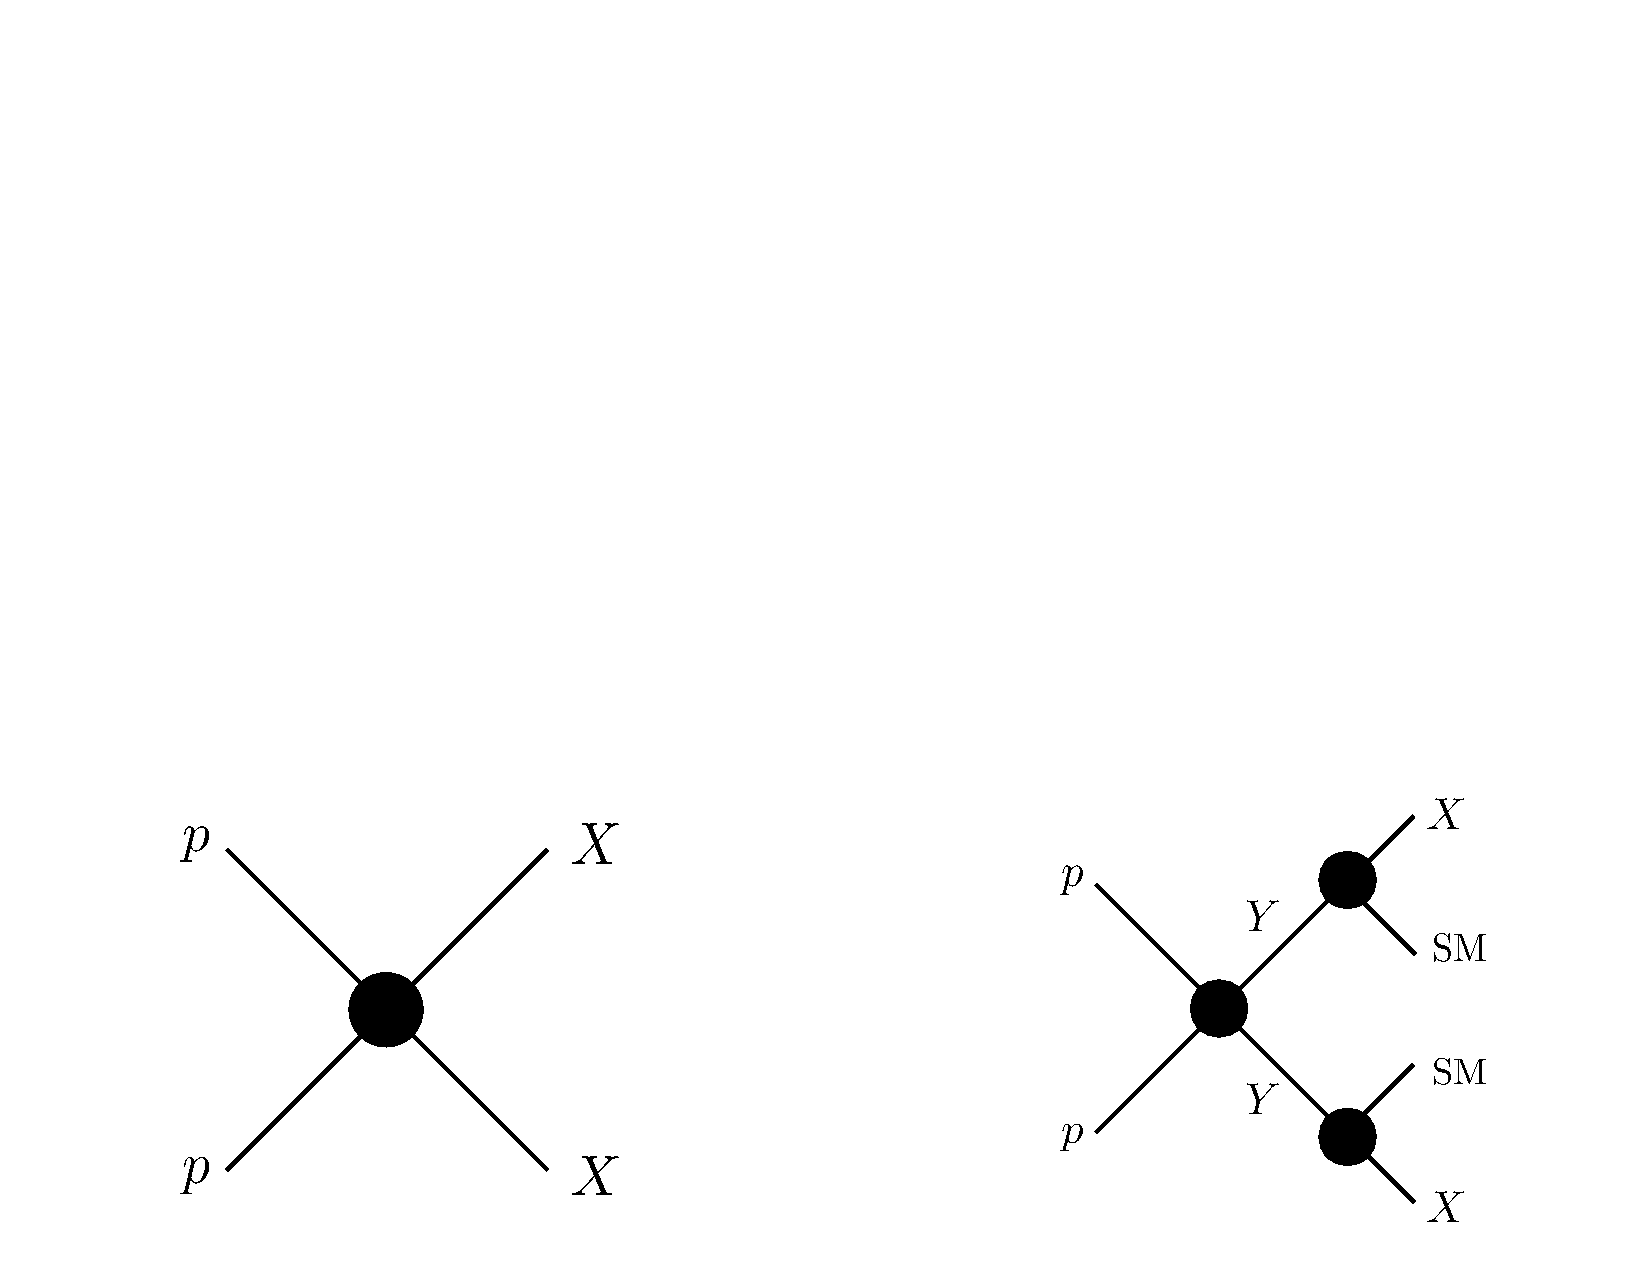
\includegraphics[width=\textwidth]{figures/feyndiagram_row1.pdf}}
\vspace{0.8cm}
\centerline{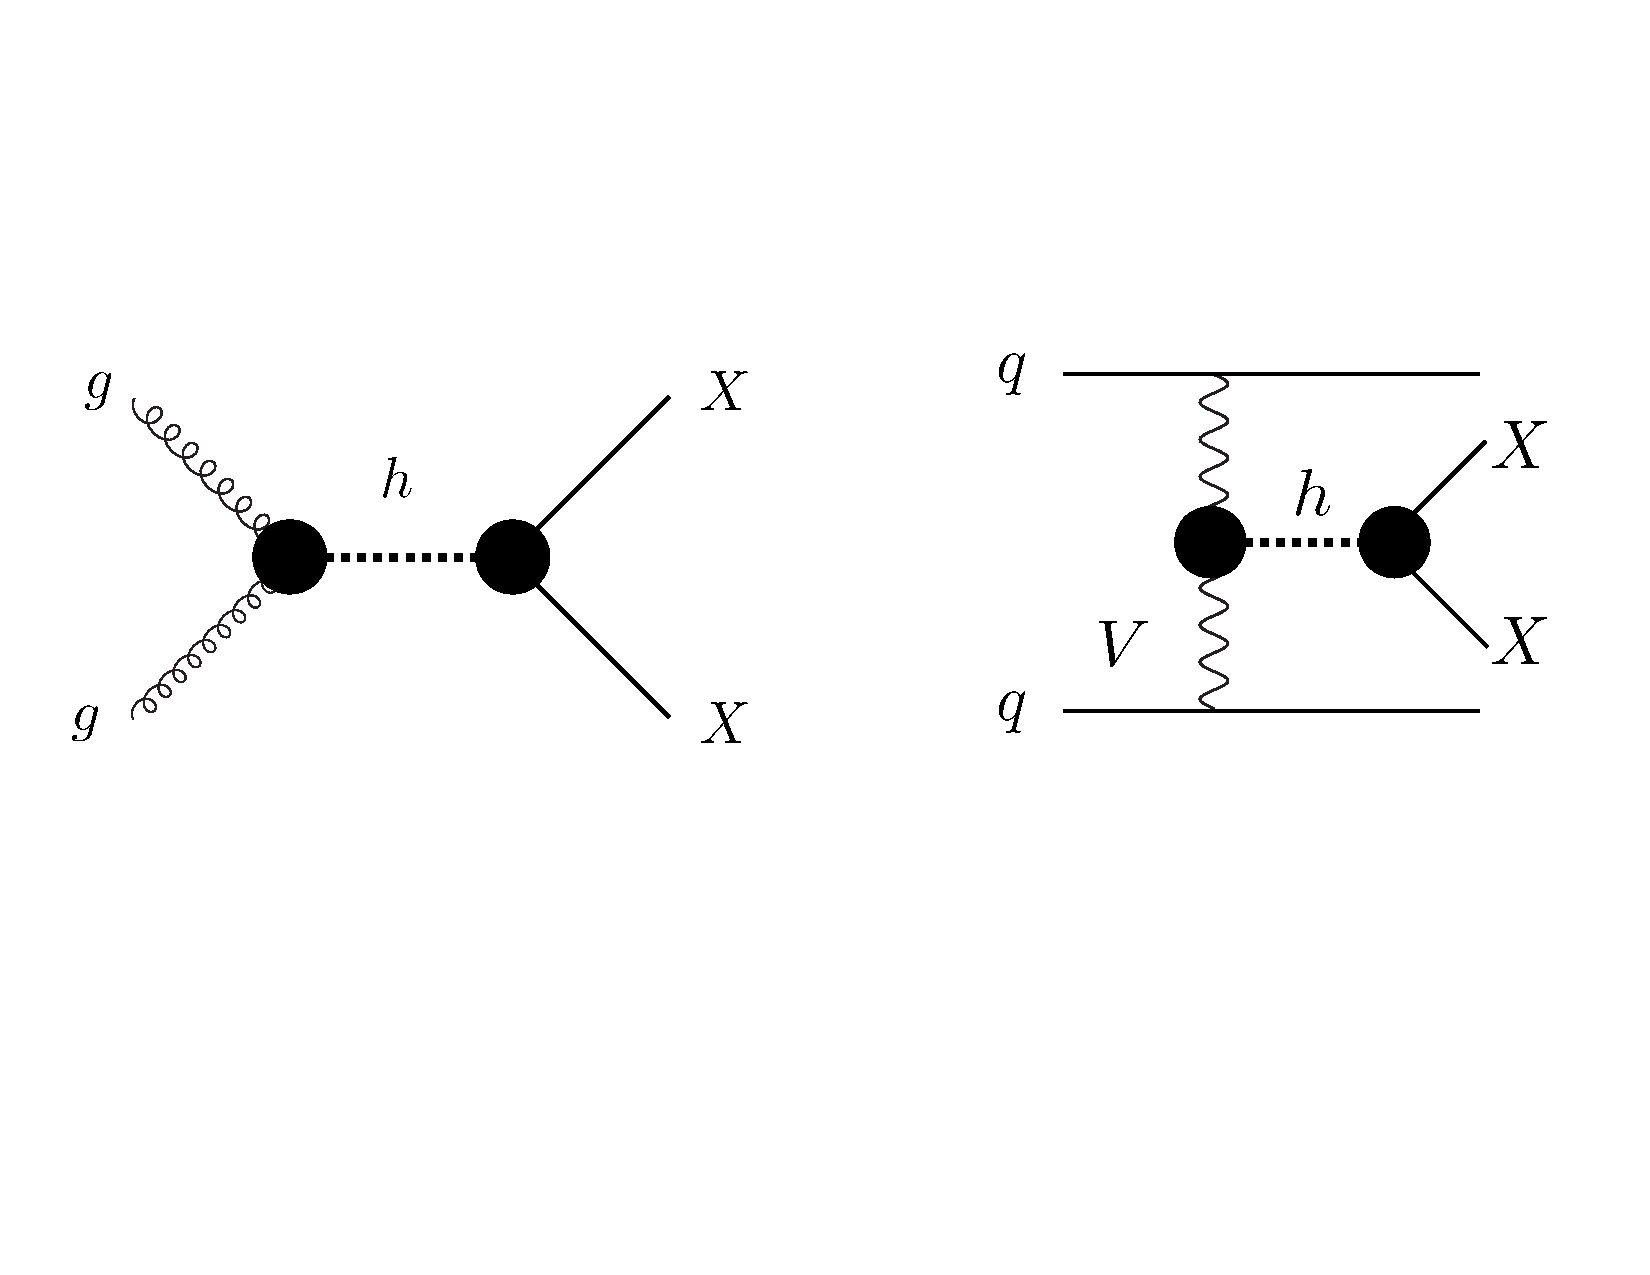
\includegraphics[width=\textwidth]{figures/feyndiagram_row2.pdf}}
\vspace{0.8cm}
\centerline{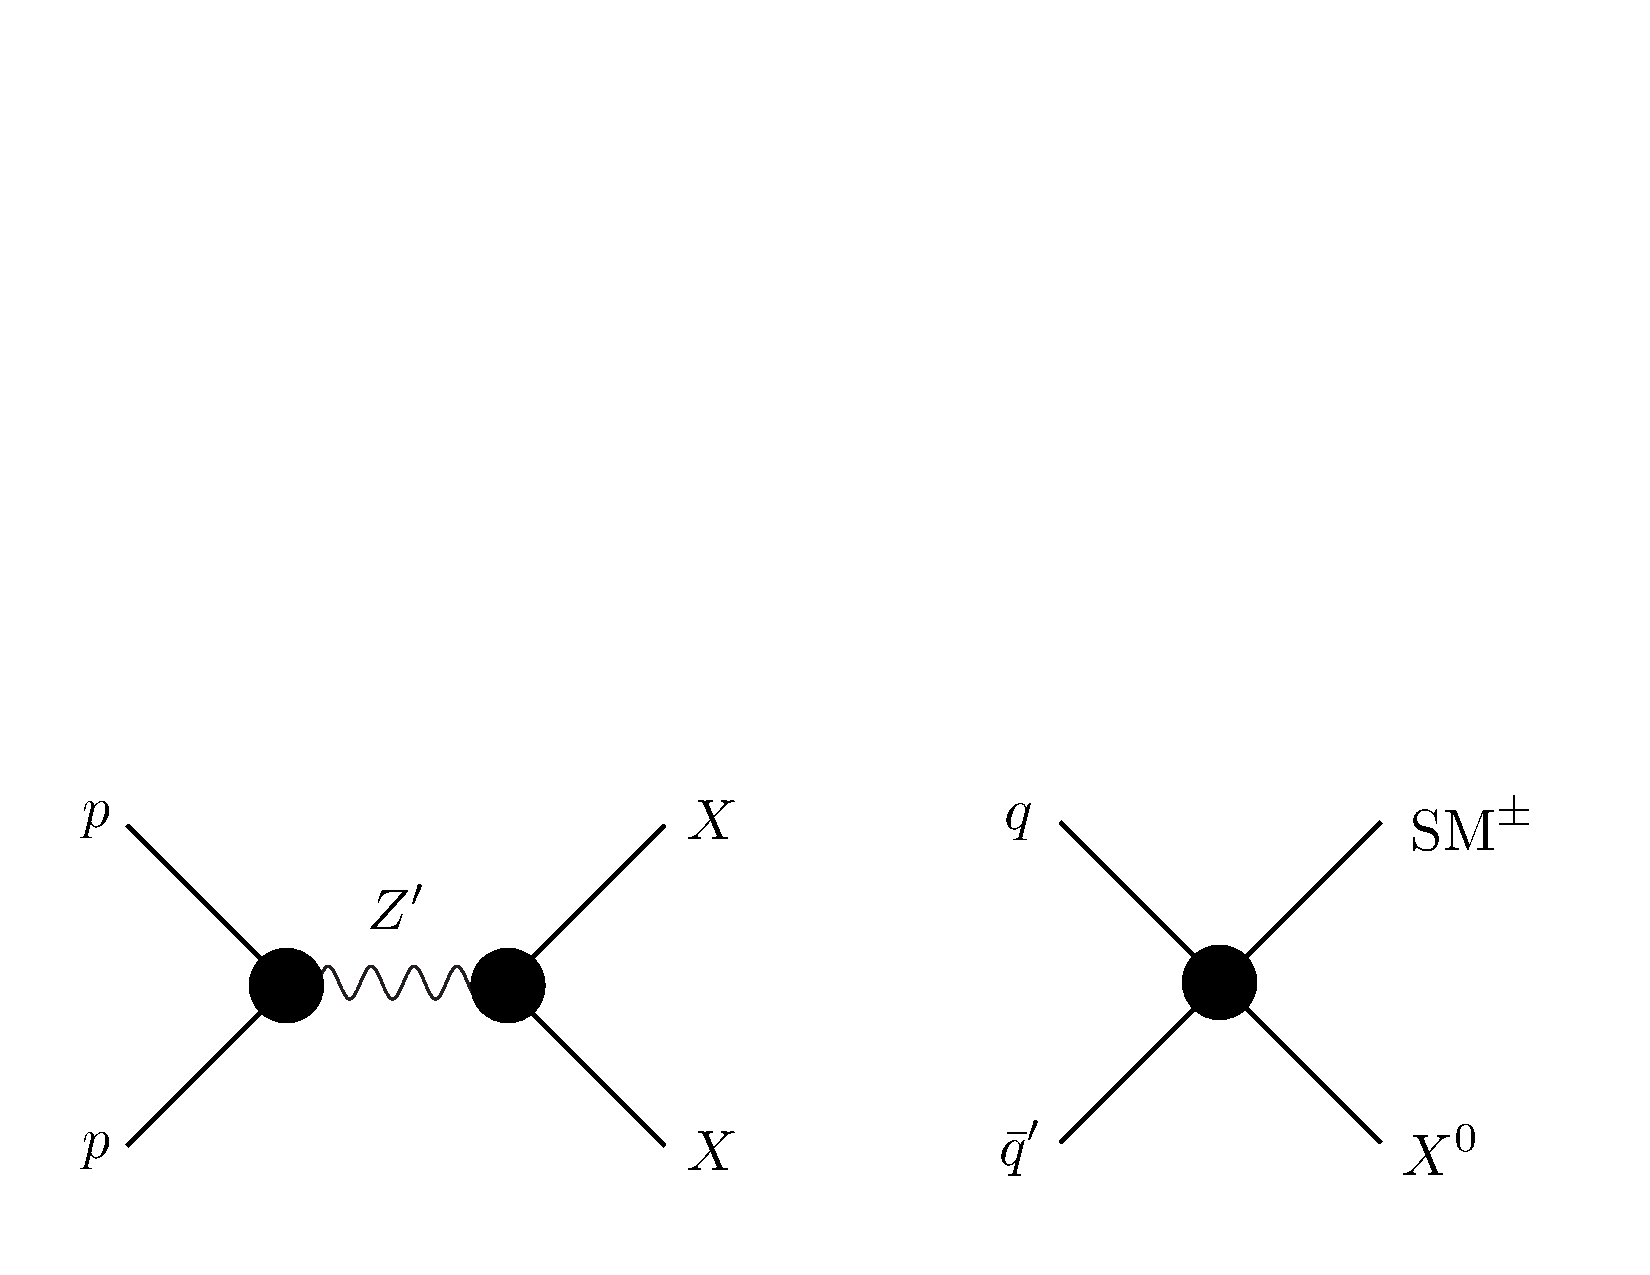
\includegraphics[width=\textwidth]{figures/feyndiagram_row3.pdf}}
  \caption{Schematic illustrations of LLP production modes in our simplified model framework. From top to bottom and left to right:~direct pair production (DPP); heavy parent (HP); Higgs modes (HIG), including gluon fusion and VBF production (not shown here is $VH$ production); heavy resonance (RES); charged current (CC).}
  \label{fig:feyndiagram}
\end{figure}
%%%%%%%%%%%%%%%%%%%%%%%%%

%
\begin{itemize}

\item {\bf Direct-Pair Production (DPP):}~here the LLP is dominantly pair-produced non-resonantly from SM initial states.
This is most straightforwardly obtained when the LLP is charged under a SM gauge interaction.  
In this case, an irreducible production cross section is then specified by the LLP gauge charge and mass.
Such continuum DPP can also occur in the presence of a (heavy, virtual) mediator (\emph{e.g.,} an initial quark$-$antiquark pair may exchange a virtual squark to pair produce bino-like neutralinos); in this case the production cross section is essentially a free parameter, as it is determined by the unknown heavy mediator masses and couplings.

\item {\bf Heavy Parent (HP):}~the LLP is produced in the decays of on-shell heavy-parent particles that are themselves pair produced from the $pp$ initial state.
The production cross section is essentially a free parameter, and is indirectly specified by the gauge charges and masses of the heavy parent particles.
Heavy-parent production gives very different kinematics for the LLP than DPP, and  often produces additional prompt AOs in the rapid cascade decays of the parents.

\item {\bf Higgs (HIG):}~here the LLP is produced through its couplings to the SM-like Higgs boson.
This case has an interesting interplay of possible production modes.
The dominant production is via gluon fusion, which features no AOs beyond gluon ISR.
Owing to its role in electroweak symmetry breaking, however, the Higgs has associated production modes (VBF, $VH$), each with its own characteristic features.
The best prospects for discovery are for LLP masses below $m_h/2$, in which case the LLPs can be in decays of the on-shell SM-like Higgs boson.
Higher-mass LLPs can still be produced via an off-shell Higgs, albeit at substantially lower rates \cite{Cui:2014twa,Craig:2014lda}.
The LLP can be pair produced or singly produced through the Higgs portal depending on the model; an LLP $X$ can also be produced in association with $\slashed{E}_{\rm T}$ via $h\rightarrow XX+\slashed{E}_{\rm T}$ or $h\rightarrow X+\slashed{E}_{\rm T}$.
The cross section (or, equivalently, the Higgs branching fraction into the LLP) is a free parameter of the model.
The Higgs mass can also be taken as a free parameter:~there exist many theories that predict new exotic scalar states (such as the singlet-scalar extension to the SM~\cite{Silveira:1985rk}), and these new scalars can be produced in the same manner as the SM Higgs.

\item {\bf Heavy Resonance (RES):}~here the LLP is produced in the decay of an on-shell resonance, such as a heavy $Z'$ gauge boson initiated by $q\bar{q}$ initial state.
Note that production via an off-shell resonance is kinematically similar to the DPP mode.
As with HIG, the LLP can be pair produced or singly produced (potentially in association with $\slashed{E}_{\rm T}$).
In RES models, ISR is the dominant source of prompt AOs.
Models with new heavy scalars could conceivably fall into either RES or HIG; the main determining factor according to our organizational scheme is whether the scalar possesses Higgs-like production modes such as VBF and $VH$.
Note that heavy resonance decays to SM particles also occur in these models, and searches for such resonances~\cite{Khachatryan:2016zqb,Sirunyan:2016iap,Aaboud:2017yvp,Sirunyan:2017dnz,Aaboud:2017buh,Aaboud:2018juj,Aaboud:2018zba} may complement the sensitivity for decays to LLPs.

\item {\bf Charged Current (CC):}~in models with weak-scale right-handed neutrinos, the LLP can be produced in the leptonic decays of $W/W'$.
Single production is favored.
Prompt charged leptons from the charged-current interaction are typical prompt AOs.
\end{itemize}
%

It is important to note that each of the above production mechanisms has its own ``natural'' set of triggers to record the signal.
For example, HIG production can be accompanied by forward jets or leptons that are characteristic of VBF or $VH$ production.
Similarly, CC production often results in prompt charged leptons, while HP production comes with AOs from the heavy-parent decay.
However, the reader should be cautioned that this does not necessarily mean that the ``natural'' trigger is \emph{optimal} for a particular signal.
For example, the HIG modes suggest the use of VBF- or $VH$-based triggers, but if the LLP decays leptonically, it might be more efficient to trigger on the lepton from the LLP decay.
Thus, the final word on which trigger is most effective for a given simplified model depends on the production mode as well as the nature and kinematics of the LLP decay.
The prompt AOs of each production mode could still, however, be used to extend sensitivity to the model (see Section~\ref{sec:ch5-smsReinterpretations}).

We also comment that some models may span several production modes.
For example, a charged LLP that is part of an electroweak multiplet and nearly degenerate with a stable, neutral component~\cite{Chen:1995yu,Thomas:1998wy,Feng:1999fu,Cirelli:2005uq,Ibe:2006de,Cirelli:2009uv,FileviezPerez:2008bj,Buckley:2009kv,Mahbubani:2017gjh} gives both DPP signatures (via $pp\rightarrow \chi^+\chi^-$) and CC production (via associated production $pp\rightarrow\chi^\pm\chi^0$).
Comprehensive coverage of each of the above production modes will allow for a conservative determination of sensitivity for models that span many production modes.

%%%%%%%%%%%%%%%%%%%%%%%%%%
\subsection{Decay Modes}\label{sec:decmodes}
%%%%%%%%%%%%%%%%%%%%%%%%%%

We now list a characteristic set of LLP decay modes.
As we attempt to construct a minimal, manageable set of decay-mode building blocks, it is important to bear in mind that a given experimental search for LLPs can frequently be sensitive to a variety of possible LLP decay modes.
As a result, it is not always necessary to perform separate searches for each possible decay mode as might otherwise be needed for prompt signatures.

The fact that LLP searches can be sensitive to many LLP decay modes is, in part, because LLPs that decay far from the collision point offer fewer avenues for particle identification.
For example, for an LLP decaying inside of the calorimeter, most decay products are reconstructed as missing energy, or an energy deposition in the calorimeter.
Consequently, particle identification criteria are typically relaxed in comparison to requirements on searches without displaced objects.
Indeed, these ``loose'' collider objects can differ significantly from the corresponding ``tight'', prompt objects.
This leads to more inclusive analyses that can cover a wider range of signatures with a single search.

Additionally, backgrounds for LLP searches are often small; for a comprehensive discussion of backgrounds to LLP searches, see Chapter~\ref{sec:backgrounds}.
As a result, tight identification and/or reconstruction criteria typically found in exclusive prompt analyses are  no longer needed to suppress backgrounds.
For example, ATLAS has a displaced vertex search sensitive to di-lepton and multi-track vertices that is relatively inclusive with respect to other objects originating from near the displaced vertex~\cite{Aad:2015rba}.
Similarly, CMS has an analysis sensitive to events with one each of a high-impact-parameter muon and electron without reconstructing a vertex or any other objects~\cite{CMS-PAS-EXO-16-022}.
For these examples, the backgrounds are sufficiently low that other requirements may be relaxed and the specific decay mode of the LLP may not be too important so long as certain objects (such as muons) are present or the decay occurs in a specific location.
An even more extreme example in this regard is the search for highly-ionizing tracks sensitive to electrically and color-charged LLPs.
While the searches are primarily targeted to detector-stable particles (heavy stable charged particles or $R$-hadrons) they can also be used to probe intermediate lifetimes for which only a certain fraction of LLPs traverse the tracker before decaying (see \emph{e.g.}~\cite{Garny:2017rxs}).
Both because of low backgrounds as well as modified particle identification criteria compared to prompt searches, LLP searches can often be inclusive and therefore covered by a more limited range of simplified models.

In some cases, however, the topology of a decay does matter.
One potentially important factor that influences the sensitivity of a search to a particular model is whether the LLP decays into two SM objects vs.~three, because the kinematics of multi-body decay are distinct from two-body decay and this may affect the acceptance of particular search strategies.
An additional simplified model featuring a three-body decay of the LLP may consequently be needed to span the space of signatures.
  
Below, we describe an irreducible set of decay modes that can be used to characterize LLP signatures for various LLP charges (including neutral, electrically charged, and color charged).
For each, we also provide an explicit example for how the decay would appear in a particular UV model.
{\bf We emphasize that the following decay modes are  loosely defined with the understanding that their signatures are also representative of similar, related decay modes; for example $2j$ or $2j+\slashed{E}_{\rm T}$ can also be proxies for $3j$ because searches for multi-body hadronic LLP decays can be sensitive to both and typically do not require reconstruction of a third jet.}
It should also be noted that we are not recommending searches to be optimized to the exact, exclusive decay mode because that could suppress sensitivity to related but slightly more complicated LLP decays.

\begin{itemize}
\item {\bf Di-photon decays:}~the LLP can decay resonantly to $\gamma\gamma$ (like in Higgs-portal models or left$-$right symmetric models~\cite{Dev:2016vle}) or to $\gamma\gamma+\mathrm{invisible}$ (in DM models).
This latter mode stands as a proxy for other $\gamma\gamma+X$ decays where the third object is not explicitly reconstructed, although whether $X$ is truly invisible can influence the triggers used.
\emph{Example:~a singlino decaying to a singlet (which decays to $\gamma\gamma$) and a gravitino in Stealth SUSY~\cite{Fan:2011yu}.}

\item {\bf Single-photon decays:}~the LLP decays to $\gamma+\mathrm{invisible}$ (like in SUSY models).
The SUSY model mandates a near-massless invisible particle, while other models (such as DM theories~\cite{Weiner:2012cb,Primulando:2015lfa}) allow for a heavy invisible particle.
\emph{Example:~a bino decaying to photon plus gravitino in gauge-mediated models of SUSY breaking~\cite{Dimopoulos:1996yq}.}
%dark matter framework can come with a heavy final state particle.

\item {\bf Hadronic decays:}~the LLP can decay into two jets ($jj$) (like in Higgs and gauge-portal models, or RPV SUSY), $jj$ + invisible (SUSY, dark matter, or neutrino models), or $j$ + invisible (SUSY).
Here, ``jet'' ($j$) means either a light-quark parton, gluon, or $b$-quark.
This category also encompasses decays directly into hadrons (for example, LLP decay into $\pi^+$ plus an invisible particle~\cite{Chen:1995yu,Thomas:1998wy,Feng:1999fu}).
\emph{Example:~a scalar LLP decaying to $b\bar{b}$ due to mixing with the SM Higgs boson, as in models of neutral naturalness~\cite{Chacko:2005pe,Burdman:2006tz,Craig:2015pha}}.

\item {\bf Semi-leptonic decays:}~the LLP can decay into a lepton + 1 jet (such as in leptoquark models) or 2 jets (like in SUSY or neutrino models).
\emph{Example:~a right-handed neutrino decaying to a left-handed lepton and an on- or off-shell hadronically decaying $W$ boson (or $W'$ boson in a left$-$right symmetric model)~\cite{Keung:1983uu}. }

\item {\bf Leptonic decays:}~the LLP can decay into $\ell^+\ell^-(+\mathrm{invisible})$, or $\ell^\pm+\mathrm{invisible}$ (as in Higgs-portal, gauge-portal, SUSY, or neutrino models).
Here the symbol $\ell$ may be any flavor of charged lepton, but the decays are lepton flavor-universal and (for $\ell^+\ell^-$ decays) flavor-conserving.
\emph{Example:~a wino decaying to a neutralino and an on- or off-shell leptonic Z boson in SUSY~\cite{Barbier:2004ez}.}

\item {\bf Flavored leptonic decays:}~the LLP can decay into $\ell_\alpha+\mathrm{invisible}$, $\ell_\alpha^+\ell_\beta^-$ or $\ell_\alpha^+\ell_\beta^-+\mathrm{invisible}$ where flavors $\alpha\neq\beta$ (as in SUSY or neutrino models).
\emph{Example:~a neutralino decaying to two leptons and a neutrino in $R$-parity-violating SUSY~\cite{Barbier:2004ez}; or a right-handed neutrino decaying to two leptons and a neutrino~\cite{delAguila:2008cj}.}
\end{itemize}

In all cases, both the LLP mass and proper lifetime are free parameters.
Therefore, the case of detector-stable particles is automatically included by taking any of the above decay modes and taking the lifetime to infinity~\footnote{As mentioned earlier, in the $c\tau\rightarrow\infty$ limit the decay mode becomes irrelevant. However, an exception is the search for particles that are stopped inside the detector material and decay out of time, which are discussed in Section~\ref{sec:outoftime}.}.
We emphasize that, depending on the location of the LLP within the detector, these decay modes may or may not be individually distinguishable:~a displaced di-jet decay will look very different from a displaced di-photon decay in the tracker, but nearly identical if the decay occurs in the calorimeter.
The goal here is to identify  promising channels (as distinct from detector signatures). 

As an example of how the above-listed decay modes cover the most important experimental signatures, we consider a scenario of an LLP decaying to top quarks.
This scenario is very well motivated (for instance, with long-lived stops in SUSY) and might appear to merit its own decay category of an LLP decaying to one or more top quarks.
However, the top quark immediately decays to final states that \emph{are} covered in the above list, giving an effective semileptonic decay mode ($t\rightarrow b\ell^+\nu$) and a hadronic decay mode ($t\rightarrow bjj$) of the LLP.
Similarly, LLP decays to four or more final states are typically covered by the above inclusive definitions of decay modes; this provides motivation not to over-optimize experimental searches to the specific, exclusive features of a particular decay mode.

While it would be ideal to have separate experimental searches for each of the above decay modes (when distinguishable), it is rare for specific models to allow the LLP to decay in only one manner; as in the  example of an LLP decaying to a top quark, a number of decay modes typically occur with specific predictions for the branching fractions.
As another example, if the LLP couples to the SM via mixing with the SM Higgs boson, then the LLP decays via mass-proportional couplings giving rise to $b$- and $\tau$-rich signatures.
If, instead, the LLP decays through a kinetic mixing as in the case of dark photons or $Z$ bosons, then the LLP can decay to any particle charged under the weak interactions, giving rise to a relatively large leptonic branching fraction in addition to hadronic decay modes.
This allows some level of prioritization of decay modes based on motivated UV-complete models; for example, the Higgs-portal model prioritizes searches for heavy-flavor quarks and leptons in LLP decay, while the gauge-portal model prioritizes searches for electrons and muons in LLP decay.
Ultimately, however, it is desirable to retain independent sensitivity to each individual decay mode as much as possible.
Indeed, for each decay mode listed above, models exist for which the given decay mode would be the main discovery channel. 
\linebreak

\noindent {\bf Invisible Final-State Particles:}~where invisible particles appear as products of LLP decays, additional model dependence arises from the unknown mass of the invisible particle.
The invisible particle could be a SM neutrino, DM, an LSP in SUSY, or another BSM particle.
The phenomenology depends strongly on the mass splitting, $\Delta \equiv M_{\rm LLP}-M_{\rm invisible}$.
If $\Delta \ll M_{\rm LLP}$ (\emph{i.e.,} $M_{\rm LLP}\sim M_{\rm invisible}$), the spectrum is compressed and the visible decay products of the LLP are soft.
This could, for instance, lead to signatures such as disappearing tracks or necessitate the use of ISR jets to trigger on the LLP signature.
If the mass splitting is large, $M_{\rm invisible}\ll M_{\rm LLP}$, then the signatures lose their dependence on the invisible particle mass.

We suggest three possible benchmarks:~a compressed spectrum with $\Delta \ll M_{\rm LLP}$ (example:~a nearly degenerate chargino-neutralino pair, giving rise to soft leptons or disappearing tracks~\cite{Chen:1995yu,Thomas:1998wy,Feng:1999fu,Cirelli:2005uq,Ibe:2006de,Cirelli:2009uv,FileviezPerez:2008bj,Buckley:2009kv,Mahbubani:2017gjh}); a massless invisible state, $\Delta = M_{\rm LLP}$ (example:~a next-to-lightest SUSY particle (NLSP) decaying to SM particles and a massless gravitino in gauge-mediated SUSY breaking~\cite{Dimopoulos:1996vz,Ambrosanio:1997rv,Delgado:2007rz,Meade:2010ji,Allanach:2015cia,Evans:2016zau,Allanach:2016pam}); and an intermediate splitting corresponding to a democratic mass hierarchy, $\Delta \approx M_{\rm LLP}/2$ (example:~NLSPs in mini-split SUSY~\cite{Arvanitaki:2012ps,ArkaniHamed:2012gw,Liu:2015bma}).

%%%%%%%%%%%%%%%%%%%%%%%%%%%%%%%%%%%%
\section{A Simplified Model Proposal}\label{sec:proposal}
%%%%%%%%%%%%%%%%%%%%%%%%%%%%%%%%%%%%

In this section, we present a compact set of simplified model channels that, broadly speaking, covers the space of theoretical models in order to motivate new experimental searches.
Such a minimal, compact set may not be optimal for reinterpretation of results (where variations on our listed production and decay modes may influence signal efficiencies and cross section sensitivities), but rather provides a convenient characterization of possible signals to ensure that no major discovery mode is missed.
These models may therefore serve as a starting point for systematically understanding experimental coverage of LLP signatures and devising new searches, but may need to be extended in future for the purposes of facilitating reinterpretation.
We undertake an in-depth discussion of these topics in Section~\ref{sec:reint}.

We classify LLPs according to their SM gauge charges, as these dictate the dominant or allowed LLP production and decay modes, and can give rise to different signatures (for example, disappearing tracks and hadronized LLPs).
We separately consider LLPs that are:~(a)~neutral; (b)~electrically charged but color neutral; and (c)~color charged.
In the latter case, it is important to distinguish between the long-lived parton (which carries a charge under quantum chromodynamics, QCD) that hadronizes prior to decay, and the physical LLP, which is a color-singlet ``$R$-hadron'' (using the standard nomenclature inspired by SUSY).
The decays of the $R$-hadron are still dominated by the parton-level processes.

All of the following models have the LLP mass and lifetime as free parameters.
For heavy-parent (HP) production, the parent mass is an additional parameter, while for invisible decays, several different benchmarks for mass splittings between LLP and invisible final state may have to be separately considered as described in Section~\ref{sec:decmodes}.
The cross section may have a theoretically well-motivated target value depending on UV-model parameters, but phenomenologically can generally be taken as a free parameter.

We emphasize that in spite of the many simplified model channels proposed below, a small number of experimental LLP searches can have excellent coverage over a wide range of channels (at least for certain lifetime ranges).
The list is intended to be comprehensive in order to identify whether there are new searches that could have a similarly high impact on the space of simplified models, and identify where the gaps in coverage are.

%%%%%%
\subsection{Neutral LLPs}\label{sec:proposal_neutralLLP}
%%%%%%

The simplified model channels for neutral LLPs are shown in Table~\ref{tab:neutral_LLP}, where $X$ indicates the LLP.

In our initial proposal, which is the first iteration of the simplified model framework, it is sufficient to consider as ``jets'' all of the following:~$j=u,d,s,c,b,g$.
It is worth commenting that $b$-quarks pose unique challenges and opportunities.
Since $b$-quarks are themselves LLPs, they appear with an additional displacement relative to the LLP decay location.
They also often give rise to soft muons in their decays, which could in principle lead to additional trigger or selection possibilities.
However, these subtleties can be addressed in further refinements of the simplified models; we discuss this further in Section~\ref{sec:simplified_future}.
Similarly, we consider $e$, $\mu$, and $\tau$ to be included in the broad category of ``leptons'', with the proviso that
searches should be designed where possible with sensitivity to each.
 
When multiple production modes are specified in one row of the table, this means that multiple especially well-motivated production channels give rise to similar signatures.
Typically only one of these simplified model production modes will actually need to be included when developing and assessing sensitivity of an experimental search, but we sometimes include multiple different production modes as individuals may variously prefer one over the other.

In each entry of the table, we indicate which umbrella category of well-motivated UV models (Section~\ref{sec:motivated_theories}) can predict a particular $(\mathrm{production})\times(\mathrm{decay})$ mode.
An asterisk (*) on the umbrella model indicates that $\slashed{E}_{\rm T}$ is required in the decay.
A dagger (${}^\dagger$) indicates that this particle production $\times$ decay scenario is not present in the \emph{simplest and most minimal} implementations or spectra of the umbrella model, but could be present in extensions of the minimal models.
While the HIG production signatures are best-motivated for the SM-like 125 GeV Higgs, exotic Higgses of other masses can still have the same production modes and so $m_H$ can be taken as a free parameter.
%
\begin{table}[t]
\begin{center}
\begin{tabular}{ |c|c|c|c|c|c|c| } 
 \hline
\backslashbox{Production}{Decay} & $\gamma\gamma(+\mathrm{inv.})$ & $\gamma+\mathrm{inv.}$ & $jj(+\mathrm{inv.})$ & $jj\ell$ & $\ell^+\ell^-(+\mathrm{inv.})$ & $\ell_\alpha^+\ell_{\beta\neq\alpha}^-(+\mathrm{inv.})$\\
 \hline\hline
 DPP:~sneutrino pair & ${}^\dagger$ & SUSY & SUSY & SUSY & SUSY & SUSY\\
 or neutralino pair &&&&&&\\
 \hline
 HP:~squark pair, $\tilde{q}\rightarrow jX$ & $ {}^\dagger$  & SUSY & SUSY & SUSY & SUSY & SUSY\\
 or gluino pair $\tilde g\rightarrow jjX$ &&&&&&\\
 \hline
 HP:~slepton pair, $\tilde{\ell}\rightarrow\ell X$ & ${}^\dagger$ & SUSY & SUSY & SUSY & SUSY & SUSY\\
 or chargino pair, $\tilde{\chi}\rightarrow WX$ &&&&&&\\
 \hline 
% HIG:~$h(h')\rightarrow XX$ & Higgs (DM)  &  & Higgs (DM) &  & Higgs (DM) & \\
 HIG:~$h\rightarrow XX$ & Higgs, DM*  & ${}^\dagger$ & Higgs, DM* & RH$\nu$ & Higgs, DM* &RH$\nu$* \\
  or $\rightarrow XX+\mathrm{inv.}$ &&&&& RH$\nu$* &\\
 \hline 
 %HIG:~$h(h')\rightarrow X+\mathrm{inv.}$ & DM  &  & DM &  & DM & \\
 HIG:~$h\rightarrow X+\mathrm{inv.}$ & DM*, RH$\nu$  & ${}^\dagger$ & DM* & RH$\nu$ & DM* &${}^\dagger$ \\
 \hline
 RES:~$Z(Z')\rightarrow XX$ & $Z'$, DM*  & ${}^\dagger$ & $Z'$, DM* & RH$\nu$ & $Z'$, DM* &$ {}^\dagger$\\
 or $\rightarrow XX+\mathrm{inv.}$ &&&&&&\\
 \hline 
 RES:~$Z(Z')\rightarrow X+\mathrm{inv.}$ & DM  & ${}^\dagger$ & DM &  RH$\nu$ & DM & ${}^\dagger$\\
 \hline
  CC:~$W(W')\rightarrow \ell X$ & ${}^\dagger$  & ${}^\dagger$ & RH$\nu$* & RH$\nu$ & RH$\nu$* & RH$\nu$* \\
 \hline
\end{tabular}
%
\end{center}
\caption{{\bf Simplified model channels for neutral LLPs.} The LLP is indicated by $X$.
Each row shows a separate production mode and each column shows a separate possible decay mode, and therefore every cell in the table corresponds to a different simplified model channel of (production)$\times$(decay).
We have cross-referenced the UV models from Section~\ref{sec:motivated_theories} with cells in the table to show how the most common signatures of complete models populate the simplified model space.
The asterisk (*) shows that the model definitively predicts missing energy in the LLP decay.
A dagger (${}^\dagger$) indicates that this particle production $\times$ decay scenario is not present in the \emph{simplest and most minimal} implementations or spectra of the umbrella model, but could be present in extensions of the minimal models.
When two production modes are provided (with an ``or''), either simplified model can be used to simulate the same simplified model channel.}\label{tab:neutral_LLP}
\end{table}

We remind the reader that the production modes listed in Table~\ref{tab:neutral_LLP} encompass also the associated production of characteristic prompt objects.
For example, the Higgs production modes not only proceed through gluon fusion, but also through VBF and $VH$ production, each of which results in associated prompt objects such as forward jets in VBF, and leptons or $\slashed{E}_{\rm T}$ in $VH$.
All of the production modes listed in Table~\ref{tab:neutral_LLP} could be accompanied by ISR jets that aid in triggering or identifying signal events.
It is therefore important that searches are designed to exploit such prompt AOs whenever they can improve signal sensitivity, especially with regard to triggering.

To demonstrate how to map full models onto the list of simplified models (and vice-versa), we consider a few concrete cases.
For instance, if we consider a model of neutral naturalness where $X$ is a long-lived scalar that decays via Higgs mixing (for instance, $X$ could be the lightest quasi-stable glueball), then the process where the SM Higgs $h$ decays via  $h\rightarrow XX$, $X\rightarrow b\bar{b}$ would be covered with the HIG production mechanism and a di-jet
decay.
Entirely unrelated models, such as the case where $X$ is a bino-like neutralino with RPV decays $h\rightarrow XX$, $X\rightarrow j jj $ could be covered with the same simplified model because most hadronic LLP searches do not have exclusive requirements on jet multiplicity.
Similarly, a hidden-sector model with a dark photon, $A'$, produced in $h\rightarrow A'A'$, $A'\rightarrow f\bar{f}$ would also give rise to the di-jet signature when $f$ is a quark, whereas it would populate the $\ell^+\ell^-$
column if $f$ is a lepton.
Finally, a scenario with multiple hidden-sector states $X_1$ and $X_2$, in which $X_2$ is an LLP and $X_1$ is a stable, invisible particle, could give rise to signatures like $h\rightarrow X_2 X_2$, $X_2\rightarrow X_1jj$ that would be covered by the same HIG production, hadronic-decay simplified model; however, we see how  $\slashed{E}_{\rm T}$ can easily appear in the final state, and that the LLP decay products may not be entirely hadronic.
Therefore, the simplified models in Table~\ref{tab:neutral_LLP} can cover an incredibly broad range of signatures, but only if searches are not overly optimized to particular features such as $\slashed{E}_{\rm T}$ and LLPs decaying entirely visibly (which would allow reconstruction of the LLP mass)~\footnote{This should not, of course, be interpreted as saying that searches shouldn't be done that exploit these features.
Instead, our position is that experiments should bear in mind the range of topologies and models covered by each cell in Table~\ref{tab:neutral_LLP} when designing searches, and that some more inclusive signal regions should be established where possible.}.

\subsection{Electrically Charged LLPs:~$|Q|=1$}\label{sec:EMcharge}

For an electrically charged LLP, we need to consider far fewer production modes because of the irreducible gauge production associated with the electric charge.
We still consider the additional possibility of a HP scenario where the parent has a QCD charge, as this could potentially dominate the production cross section, see \emph{e.g.}, Ref.~\cite{Heisig:2012zq}.
We summarize our proposals in Table~\ref{tab:charged_LLP}.

Note that we group all resonant production into the $Z'$ simplified model.
The reason is that the SM Higgs cannot decay into two on-shell charged particles due to the model-independent limits from LEP on charged particles masses, $M\gtrsim$75$-$90 GeV (see, for example, Ref.~\cite{Abbiendi:2003yd}); because of this lower limit on the LLP mass, it is less important to use AOs for triggering and reconstructing charged LLP signatures than for neutral LLPs.
Additionally, there are fewer allowed decay modes because of the requirement of charge conservation. 

For concreteness, we recommend using $|Q|=1$ as a benchmark for charged LLPs for the purpose of determining allowed decay modes.
Although other values of $Q$ are possible, these often result in cosmologically stable charged relics or necessitate different decay modes than those listed here.
Additionally, LLPs with $|Q|=1$ are motivated within SUSY~\cite{Chen:1995yu,Thomas:1998wy,Feng:1999fu,Jittoh:2005pq,Brandenburg:2005he,Heisig:2013rya} and within Type-III seesaw models of neutrino masses~\cite{Bajc:2006ia,Bajc:2007zf,Franceschini:2008pz,Arhrib:2009mz}.
We note that there exist already dedicated searches for heavy quasi-stable charged particles with non-standard charges~\cite{Aad:2015kta,Khachatryan:2016sfv}.
Because such searches are by construction not intended to be sensitive to the decays of the LLP, the existing models are sufficient for characterizing these signatures and they do not need to be additionally included in our framework.

For massive particles with $|Q|=1$ with intermediate or large lifetimes such that the LLP traverses a significant part (or all) of the tracker, the highly ionizing track of the LLP provides a prominent signature.
This can be exploited for an efficient suppression of backgrounds while keeping identification and/or reconstruction criteria as loose and, hence, as inclusive as possible.
In particular, for decay-lengths of the order of or larger than the detector size, the signature of highly ionizing tracks and anomalous time of flight (\emph{i.e.,}~searches for heavy stable charged particles; see Sections~\ref{subsec:funnytracks} and~\ref{sec:ch5-HSCPs}) constitute an important search strategy covering a large range of lifetimes present in the parameter space of theoretically motivated models.
While the searches for heavy stable charged particles are largely inclusive with respect to additional objects in the event, they depend strongly on the velocity of the LLP\@.
For $\beta\to1$ one loses the discriminating power against minimally ionizing particles, while for small velocities, $\beta\lesssim0.5$, the reconstruction becomes increasingly difficult due to timing issues.
It is therefore important to include the heavy parent production scenario which covers a much larger kinematic range than direct production alone and which may feature a much wider range of signal efficiencies than the DPP scenario~\cite{Heisig:2015yla}.

\begin{table}[t]
\begin{center}
\begin{tabular}{ |c|c|c|c|c|} 
 \hline
\backslashbox{Production}{Decay} & $\ell+\mathrm{inv.}$ &  $jj(+\mathrm{inv.})$ & $jj\ell$ & $\ell\gamma$ \\
\hline\hline
DPP:~chargino pair & SUSY & SUSY & SUSY & ${}^\dagger$ \\
or slepton pair & DM* & DM* & &\\
\hline
HP:~$\tilde{q}\rightarrow j X$ & SUSY & SUSY & SUSY &${}^\dagger$ \\
& DM* & DM* & &\\
\hline
RES:~$Z'\rightarrow XX$ & Z', DM*& Z', DM* & Z'  &${}^\dagger$ \\
\hline
CC:~$W'\rightarrow X+\mathrm{inv.}$ & DM* & DM* & RH$\nu$ &${}^\dagger$\\
\hline
\end{tabular}
\end{center}
\caption{{\bf Simplified model channels for electrically charged LLPs} such that $|Q| = 1$.
The LLP is indicated by $X$.
Each row shows a separate production mode and each column shows a separate possible decay mode, and therefore every cell in the table corresponds to a different simplified model channel of (production)$\times$(decay).
We have cross-referenced the UV models from Section~\ref{sec:motivated_theories} with cells in the table to show how the most common signatures of complete models populate the simplified model space.
The asterisk (*) shows that the model definitively predicts missing energy in the LLP decay.
A dagger (${}^\dagger$) indicates that this particle production $\times$ decay scenario is not present in the \emph{simplest and most minimal} implementations or spectra of the umbrella model, but could be present in extensions of the minimal models.
When two production modes are provided (with an ``or''), both production simplified models can be used to cover the same experimental signatures.}\label{tab:charged_LLP}
\end{table}

While the signatures in Table~\ref{tab:charged_LLP} form a minimal set, they also encompass some scenarios that merit special comment.
One of these is the disappearing track signature~\cite{Chen:1995yu,Thomas:1998wy,Feng:1999fu,Cirelli:2005uq,Ibe:2006de,Cirelli:2009uv,FileviezPerez:2008bj,Buckley:2009kv,Mahbubani:2017gjh}, in which a charged LLP decays to a nearly degenerate neutral particle.
The lifetime is long in this scenario due to the tiny mass splitting between the two states.
Formally, these are included in the chargino or slepton DPP modes in Table~\ref{tab:charged_LLP} with decays to $\ell+\mathrm{inv.}$ or $q\bar{q}'+\mathrm{inv.}$ taken in the limit where the splitting between the charged LLP and the invisible final state is of $\mathcal{O}(200\,\,\mathrm{MeV})$.
In the case of a hadronic decay, $X$ decays to a soft pion that is very challenging to reconstruct and so the track simply disappears.
This is an important scenario that is already the topic of existing searches~\cite{CMS:2014gxa,Aaboud:2017mpt}.
As the degeneracy between the charged LLP and the neutral state is relaxed, other signatures are possible; this parameter range is well motivated both by SUSY and DM models with coannihilation~\cite{Griest:1990kh,Baker:2015qna,Khoze:2017ixx}.

Finally, we comment on the challenges of simulating the charged LLP simplified models.
Because the LLP bends and interacts with detector material prior to its decay, the simulation of the LLP propagation is important in correctly modeling the experimental signature.
The subsequent decay of the LLP must either be hard-coded into the detector simulation, or allow for an interface with programs such as Pythia 8 to implement the decays.
We discuss the challenges of simulating signals for LLPs with electric or color charge in Section~\ref{sec:geant}.

\subsection{LLPs with Color Charge}
\label{sec:coloredLLPs}

An LLP charged under QCD is more constrained than even electrically charged LLPs.
Because of the non-Abelian nature of the strong interactions, the gauge pair-production cross section of the LLP is specified by the LLP mass and its representation under the color group, $\mathrm{SU}(3)_{\rm C}$.
We do not consider LLP production via a heavy parent particle  because that cross section is unlikely to dominate the total production rate at the LHC relative to DPP. The simplified model channels are provided in Table~\ref{tab:color_LLP}.

\begin{table}[t]
\begin{center}
\begin{tabular}{ |c|c|c|c|c|}
 \hline
\backslashbox{Production}{Decay} & $j+\mathrm{inv.}$ &  $jj(+\mathrm{inv.})$ & $j\ell$ & $j\gamma$ \\
\hline\hline
DPP:~squark pair & SUSY & SUSY & SUSY &${}^\dagger$ \\
or gluino pair & & & &\\
\hline
\end{tabular}
\end{center}
\caption{{\bf Simplified model channels for LLPs with color charge.} The LLP is indicated by $X$.
Each row shows a separate production mode and each column shows a separate possible decay mode, and therefore every cell in the table corresponds to a different simplified model channel of (production)$\times$(decay).
We have cross-referenced the UV models from Section~\ref{sec:motivated_theories} with cells in the table to show how the most common signatures of complete models populate the simplified model space.
A dagger (${}^\dagger$) indicates that this particle production $\times$ decay scenario is not present in the \emph{simplest and most minimal} implementations or spectra of the umbrella model, but could be present in extensions of the minimal models.
When two production modes are provided (with an ``or''), both production simplified models can be used to cover the same experimental signatures.}\label{tab:color_LLP}
\end{table}

A complication of the QCD-charged LLP is that the LLP hadronizes prior to its decay, forming an $R$-hadron bound state.
The modeling of hadronization and subsequent propagation is directly related to many properties of the long-lived parton, such as electric charge, flavor, and spin. Event generators such as Pythia 8 have routines~\cite{Sjostrand:2007gs,Sjostrand:2014zea} to simulate LLP hadronization, although it is unclear how precise these predictions are.
For a point of comparison, using the default settings of Pythia 8 yields an estimate of the neutral $R$-hadron fraction from a gluino (color-octet fermion, $\tilde g$) of approximately 54\%, while the neutral $R$-hadron fraction for a stop (scalar top partner) is estimated to be 44\%~\cite{Liu:2015bma}. After hadronization, the charge of the $R$-hadron may change as it passes through the detector. For instance, some estimates~\cite{Buccella:1985cs,Farrar:2010ps} suggest that heavy, color-octet gluinos $\tilde g$ would predominantly form mesons (\emph{e.g.,}  $(u \tilde g \bar d)$) at first.
They eventually drop to the lower-energy neutral singlet baryon $\tilde \Lambda = (\tilde g u d s)$ state when interacting with the protons and neutrons within the calorimeters.

The modeling of LLP hadronization and propagation is crucial to designing searches for color-charged LLPs and assessing their sensitivity. For example,  only the charged $R$-hadrons can be found in heavy stable charged particle search; if the LLP charge changes as it passes through the detector, heavy stable charged particle searches may have limited sensitivity. To take this into account, the experimental searches  include both tracker-only or tracker$+$calorimeter signal regions~\cite{Aaboud:2016uth,CMS-PAS-EXO-16-036}, which enhances sensitivity to the scenario in which $R$-hadrons lose their charge by the time they reach the calorimeters. 

Because no $R$-hadrons have been discovered to date and hence their properties cannot be directly measured, $R$-hadron modeling in detector simulations is challenging. We discuss  the challenges of simulating the propagation and decays of  LLPs with color charge in Section~\ref{sec:geant}.






\section{Proposal for a Simplified Model Library}\label{sec:library}

The simplified models outlined in the above sections provide a common language for theorists and experimentalists to study the sensitivity of existing searches, propose new search ideas, and interpret results in terms of UV models.
Each of these activities demands a simple framework for the simulation of signal events that can be used to evaluate signal efficiencies of different search strategies and map these back onto model parameters.
Requiring individual users to create their own MC models for each simplified model is impractical, redundant, and invites the introduction of errors into the analysis process.

In this section, we propose and provide a draft version of a \emph{simplified model library} consisting of model files and MC generator cards that can be used to generate events for various simplified models in a straightforward fashion.
Because each experiment uses slightly different MC generators and settings, this allows each collaboration (as well as theorists) to generate events for each simplified model based on the provided files.
Depending on how the LLP program expands and develops over the next few years, it may become expedient to expand the simplified model library to include sets of events in a standard format (such as the Les Houches format~\cite{Alwall:2006yp}) that can be directly fed into event-generator and detector-simulation programs.
Given the factorization of production and decay of LLPs that is valid for neutral LLPs, this could involve two mini-libraries:~a set of production events for LLPs and a set of decay events for LLPs, along with a protocol for ``stitching'' the events together.

The current version of the library is available at the LHC LLP Community website~\footnote{\url{http://cern.ch/longlivedparticles}}, hosted at CERN.
In Appendix~\ref{sec:library_more}, we also provide tables that list how to simulate each LLP simplified model channel with one of the specified base models.
These proposals are based on the models outlined in Section~\ref{sec:base} and often match the best-motivated simplified models from Section~\ref{sec:proposal}, and also building on the DM-inspired LLP simplified models proposed and detailed in Ref.~\cite{Buchmueller:2017uqu}.
The library currently focuses on models of neutral LLPs; simulating the propagation of charged LLPs along with the full range of decays listed in Sections~\ref{sec:EMcharge}$-$\ref{sec:coloredLLPs} requires more careful collaboration with detector simulation and other MC programs to ensure that they can practically be used in experimental studies.

We provide model files in the popular Universal Feynrules Output (UFO) format~\cite{Degrande:2011ua}, which is designed to interface easily with parton-level simulation programs such as MadGraph5\_aMC@NLO~\cite{Alwall:2014hca}.
The goal is to cover as many of the simplified models of Section~\ref{sec:proposal} with as few UFO models as possible; this limits the amount of upkeep needed to maintain the library and develops familiarity with the few UFO models needed to simulate the LLP simplified models.
We provide specific instructions for how to simulate each simplified LLP channel along with the UFO models. 

\subsection{Base Models for Library}\label{sec:base}

In order to reproduce the simplified model channels of Section~\ref{sec:building_blocks}, we need a collection of models that:
%
\begin{itemize}
\item Includes additional gauge bosons and scalars to allow vector- and scalar-portal production of LLPs (RES and HIG);
\item Includes new gauge-charged fermions and scalars to cover direct and simple cascade production modes of LLPs (DPP and HP); 
\item Includes a RHN-like state with couplings to SM neutrinos and leptons (CC);
\item \emph{Recommended, but optional:}~allows for the decays of the LLP particle through all of the decay modes listed in Section~\ref{sec:building_blocks}, either through renormalizable or higher-dimensional couplings.
If couplings that allow LLP decay are included in the UFO model, then the decays can be performed directly at the matrix-element level in programs such as MadGraph5\_aMC@NLO~\cite{Alwall:2014hca} and accompanying packages such as MadSpin~\cite{Artoisenet:2012st}. Alternatively, it is possible for neutral LLPs to simulate the production and decay as a single process; in such cases, numerical instabilities sometimes arise, for which dedicated event generators are needed \cite{Nemevsek:2018bbt,}.
If the couplings needed for LLP are not in the UFO model, then LLPs can be left stable at the matrix-element level and decays implemented via Pythia 8~\cite{Sjostrand:2007gs,Sjostrand:2014zea}, which allows for the straightforward implementation of decays according to a phase-space model, but does not correctly model the angular distribution of decay products.
Instructions for implementing decays in Pythia are included with the model library files.
\end{itemize}

Fortunately, an extensive set of UFO models is already available for simulating the production of BSM particles.
We note that extensions or generalizations of only three already-available UFO models are needed at the present time; the SUSY models
in particular can cover many of the simplified models since they contain an enormous collection of new fermions and scalars.
We also provide an optional
fourth model, the Hidden Abelian Higgs Model, that can be helpful to simulate HIG and ZP theories.

\begin{enumerate}

\item {\bf The Minimally Supersymmetric SM (MSSM):}~the use of this model is motivated by and allows for the simulation of SUSY-like theories.
The model contains a whole host of new particles with various gauge charges and spins.
Therefore, an MSSM-based model allows for the simulation of many of the simplified model channels.
In particular, we note that existing UFO variants of the MSSM that include gauge-mediated supersymmetry breaking (GMSB) couplings (including decays to light gravitinos), $R$-parity violation (making unstable the otherwise stable LSPs \cite{Barbier:2004ez,LopezFogliani:2005yw,Ghosh:2017yeh}), and the phenomenological MSSM (pMSSM)~\cite{Djouadi:1998di,Berger:2008cq} already cover most of the SUSY-motivated LLP scenarios. In some cases, the model is modified to give direct couplings between the Higgs states and gluons/photons.



\item {\bf The Left$-$Right Symmetric Model (LRSM):}~this UFO model is best for simulating UV theories with right-handed neutrinos (RH$\nu$).
The UFO model supplements the SM by an additional $\mathrm{SU}(2)_{\rm R}$ symmetry, which gives additional charged and neutral gauge bosons.
The model is available in the simplified models library and contains a right-handed neutrino which is the typical LLP candidate. The LLP  can be produced via SM $W$, $Z$, or via the new gauge and Higgs bosons (both charged and neutral) present in the theory~\footnote{Additional LRSM tools are available at \url{https://sites.google.com/site/leftrighthep/}.}. The LRSM therefore contains many of the charged and neutral current LLP production processes outlined in Section \ref{sec:proposal_neutralLLP}.

\item {\bf Dark-Matter Simplified Models (DMSM)}:~these UFO models are best for simulating UV theories in the DM class.
These UFO models have been created by the LHC DM working group~\cite{Abdallah:2015ter}.
They typically consist of a new BSM mediator particle (such as a scalar of a $Z'$) coupled to invisible DM particles.
The UFO models can either be modified to include an unstable LLP, or else the otherwise stable ``DM'' particle can be decayed via Pythia.
The utility and applicability of the DM simplified model framework to LLPs has already been demonstrated with a detailed proposal and study of classes of DM simplified models for LLPs~\cite{Buchmueller:2017uqu}.
These models are particularly good for simulating LLP production via a heavy resonance (RES), and can also simulate continuum production of LLPs in the limit where the mediator is taken to be light and off-shell (DPP).

\item{\bf (optional) The Hidden Abelian Higgs Model (HAHM):}~this UFO model contains new scalars and gauge bosons and so can be used to simulate both Higgs-portal and gauge-portal (ZP) theories.
The model consists of the SM supplemented by a ``hidden sector'' consisting of a new $\mathrm{U}(1)$ gauge boson and a corresponding Higgs field.
The physical gauge and Higgs bosons couple to the SM via kinetic and mass mixing, respectively.
The HAHM allows for straightforward simulation of Higgs-portal production of LLPs, as well as $Z'$ models and many hidden sector scenarios.
The UFO implementation is from Ref.~\cite{Curtin:2014cca}.

\end{enumerate}
%
If additional decay modes are needed beyond those in the specified simplified models, then the library can be updated to include the new couplings mediating the decay.
Alternatively, the LLPs can be left stable at parton level and decayed in event generators such as Pythia.


A detailed list of processes that can be used to simulate each simplified model channel is provided in Appendix~\ref{sec:library_more}.
The primary purpose of the library is to be used to simulate events for determining acceptances, and, as a result, the signal cross section is not important.
Thus, for example, SM gauge interactions can be used as proxies for much weaker exotic interactions.
Similarly, the spins of the particles are generally of subdominant importance:~replacing the direct production of a fermion with the direct production of a scalar will not fundamentally alter the signature.
As long as results are expressed in terms of sensitivity to cross sections and not couplings, the results can be qualitatively (and in many cases, quantitatively) applied to any similar production mode regardless of spin.
However, we caution the reader that changing the spin of the LLP (or its parent) can change the angular distribution, and since in some cases LLP searches are typically more sensitive to aspects of event geometry than prompt searches, the second-order effects of spin could have more of an effect than for prompt simplified models.

\subsection{LLP Propagation and Interaction with Detector Material}\label{sec:geant}

Long-lived particles with electric or QCD charges interact with the detector material prior to decay, and their propagation through the detector must be correctly modeled.
The propagation of both LLPs with color charge (in the form of $R$-hadrons) and electrically charged LLPs can be implemented in the Geant4 (G4) toolkit~\cite{Agostinelli:2002hh}.
For example, routines exist to simulate the propagation of color-charged LLPs~\cite{Mackeprang:2006gx,Mackeprang:2009ad}.
G4 also includes routines that can implement $N$-body decays of LLPs using a phase-space model.
This works fine for decays of LLPs to leptons, photons, invisible particles such as neutrinos, as well as exclusive hadronic decays. 

However, G4 cannot implement decays to partons that subsequently shower and hadronize.
One solution to this limitation is employed by CMS~\cite{Khachatryan:2015jha,Sirunyan:2017sbs} and ATLAS~\cite{Aad:2013gva} in their searches for stopped LLPs.
In these analyses, the signal simulation proceeds in two stages.
During the first stage, the production of the LLP and its subsequent interactions with the detector are simulated.
Once the stopping point of the LLP is determined, a new event is simulated including the LLP decay; the LLP decay products are then manually moved to the stopping point from the first stage.
G4 is then run a second time to determine the efficiency for reconstructing the LLP decay signal.

It would be preferable to fully automate the simulation of decays of charged LLPs after propagation in G4.
There exists in G4 a class called G4ExtDecayer, which can be used to implement decays by interfacing with an external generator.
This class has been used to interface G4 with Pythia 6~\footnote{See \url{http://geant4-userdoc.web.cern.ch/geant4-userdoc/Doxygen/examples_doc/html/Exampledecayer6.html}}.
The interface with Pythia 6 has been used most recently to model LLP gluino propagation and decay in a search for displaced vertices and missing energy in ATLAS~\cite{Aaboud:2017iio}.
Work is ongoing to extend this functionality to Pythia 8 and to simplify the interface.

An additional challenge of simulating LLP decays is that, if the LLP undergoes a multi-body decay, generators such as Pythia use a phase-space model to implement the decays. If more accuracy is required, it may be preferable to use the full matrix element via generators such as MadGraph5~\cite{Alwall:2011uj,Alwall:2014hca}. If the matrix element is important for computing the decay of the LLP, then either an interface with MadGraph is needed to implement the decay prior to passing the vertex back to Pythia 8 for showering and hadronization, or matrix-element-based methods within the event generator itself must be used.

Because of the need to interface with G4 in simulating the decays of LLPs with electric or color charges, we do not at this point include such decay modes in our simplified model library.
The decays of such LLPs will be most easily simulated via an interface with Pythia 8 once it is finalized.

Finally, we comment that LLPs can have even stranger propagation properties than  LLPs with electric or color charges.
For example, quirks are LLPs that are charged under a hidden-sector gauge interaction that confines at macroscopic scales \cite{Kang:2008ea}.
Because the confinement scale can be just about any distance, quirks can have very unusual properties; as a specific example, if electrically charged quirk-antiquirk pairs are bound on the millimeter or centimeter level, they behave as an electric dipole and therefore do not leave conventional tracks that bend in the magnetic field.
Other confinement scales give rise to different behaviors, such as meta-stable heavy charged particles and non-helical tracks~\cite{Farina:2017cts,Knapen:2017kly}.
In scenarios where the quirks carry color charge, the quirks hadronize and can undergo charge-flipping interactions as they move through the detector.
These quirk scenarios can be challenging to model, and no public code exists that allows for the propagation and interaction of quirks with the detector material; we encourage the collaborations to validate and release any internal software they may have to study the propagation of quirks (for more discussion, see the discussion of quirks  in Section~\ref{subsec:funnytracks})~\footnote{Ideally, this software would be well-documented to facilitate sharing between experiments.
A successful example of readily shareable software between experiments is the G4 package for $R$-hadrons and other particles' interaction with matter, found at~\url{http://r-hadrons.web.cern.ch/r-hadrons/}}.




\section{Limitations of Simplified Models \& Future Opportunities}\label{sec:simplified_future}

We conclude our discussion of simplified models with a more extensive discussion of the limitations of the current simplified model proposal in its application to models of various types, along with opportunities for future development.
The presented framework is only the first step of a simplified model program that is comprehensive in terms of generating LHC signatures and  allowing straightforward reinterpretation of experimental results for UV models.
The framework we have developed with separate, modular components for LLP production and decay is amenable to expansion, and we encourage members of the theory and experimental communities to continue to do so over the coming years to ensure maximal utility of the simplified models framework.

One significant simplification we have undertaken in our framework is to define a ``jet'' as any of $j=u,c,d,s,b,g$.
In reality, different partons give rise to different signatures, especially when one of the ``jets'' is a heavy-flavor quark.
Jets initiated by $b$ and $c$ quarks have some useful distinguishing features, such as the fact that the underlying heavy-flavor meson decays at a distance slightly displaced from the proton interaction vertex and that there are often associated soft leptons resulting from meson decays.
In particular, it is possible that the soft muons associated with $B$-meson decays could be used to enhance trigger and reconstruction prospects for LLPs decaying to $b$-jets~\cite{Aad:2013txa}.
However, heavy quarks also constitute an important backgrounds for LLP searches, and so LLPs decaying to $b$- and $c$-jets may necessitate dedicated treatment in future.
Similarly, LLP decays to $\tau$ leptons may merit further specialized studies.

Another property of the current framework is that it is restricted to LLP signatures of low multiplicity.
By ``low multiplicity'', we mean collider signatures with one or two LLPs.
Searches inspired by these models are also suitable for many scenarios with three or four LLPs per event (which include models with dark-Higgs decays into lepton-jets~\cite{Falkowski:2010cm}, or left$-$right symmetric models~\cite{Nemevsek:2016enw}), since the LLP signatures are generally extremely rare and so only one or two typically need to be identified in a given event to greatly suppress backgrounds.
Thus, as long as the search is inclusive with respect to possible additional displaced objects, the signature can be covered with low-multiplicity strategies.
As the LLP multiplicity grows, however, the simplified model space we have presented requires modification.
This is both because the individual LLPs grow softer, making them harder to reconstruct on an individual level, and they become less separated in the detector, which makes isolation and identification of signal a challenge.
On the other hand, the high LLP multiplicity may allow for new handles for further rejecting backgrounds, and the kinematics can vary widely based on the model (for example, in some ``quirky'' scenarios, LLPs can be produced in a variety of ways with different kinematic distributions~\cite{Beauchesne:2017ukw}). 
In extreme cases, signals can even mimic pile-up~\cite{Knapen:2016hky}.
High-multiplicity signatures therefore require dedicated modeling, and we defer the study of these signatures to Chapter~\ref{sec:showers}.


Finally, we conclude by noting that simplified models are intended to provide a general framework to cover a broad swath of models.
Any simplified model set-up, however, cannot cover every single UV model without becoming as complex as the UV model space itself. As with the case of promptly decaying new particles, care must also be taken in the interpretation of simplified models~\cite{Alves:2011wf,Abdallah:2015ter,Abercrombie:2015wmb,Boveia:2016mrp,Ambrogi:2017lov}:~for example, constraints on simplified models assuming 100\% branching fractions of LLPs to a particular final state may not accurately represent the constraint on a full model due to the large multiplicity of possible decay modes.
There will additionally always be very well-motivated models that predict specific signatures that are challenging to incorporate into the simplified model framework outlined here.
Experimental searches for these signatures should still be done where possible, but we encourage theorists and experimentalists alike to think carefully about how to design such searches so as to retain maximal sensitivity to simplified models that may give rise to similar signatures.


\chapter{Experimental Coverage}
\noindent {\bf Chapter editors:}~Xabier Cid Vidal, Heather Russell, Albert de Roeck, Jared Evans, David Curtin, Jose Zurita\\
\text{ \; }\\
\noindent {\bf Contributors:}~Juliette Alimena, Alberto Escalante del Valle, Philippe Mermod, Antonio Policchio, Brian Shuve\\
\text{ \; }\\

\noindent The goal of this chapter is to assess the capabilities of the existing long-lived particle searches at ATLAS, CMS and LHCb, and to identify any potential gaps in coverage.  We address this chapter to a reader interested in understanding the coverage of the LHC on LLPs, but assume little to no background on the search strategies, thus we include a high level of detail regarding the current analyses. While we focus on the current existing studies, we acknowledge the landscape for new physics models and LLP signatures can be broader than the ones described here.

Backgrounds to most of these studies are typically small, as there are no irreducible SM processes that mimic the exact signature.  The rare backgrounds that can fall within the signal regions, such as cosmic muons, beam halo, detector noise, and cavern backgrounds, will be discussed in detail in Chapter~\ref{sec:backgrounds}. As rare as these backgrounds are, their rate is not completely negligible, and the difficulty of modeling them usually requires additional selection requirements (e.g: LLP mass range, specific decay modes) to ensure the search can be effectively ``background-free''. 

Triggering is particularly challenging for LLP searches. With the exception of certain dedicated ATLAS triggers in the calorimeters or muon systems, there are no Level-1 (L1) triggers ( that pick up on the displaced nature of the LLP decay directly, and standard objects like leptons or high-energy jets have to pass L1 trigger thresholds in order for the event to be recorded. Hence the design of customized LLP triggers is to be encouraged, as they can probe otherwise inaccessible regions of parameter space.

A detailed review of all existing searches is presented in Section~\ref{sec:survey}.
This survey of the current experimental coverage aims to highlight the highest-priority searches needed, which are shown in Section~\ref{sec:covgaps}.
In all cases, we focus on the latest version of each analysis, notably we will typically present searches based on data taken at a center-of-mass energy $\sqrt{s}=13$ TeV,  and discussing searches using Run-1 data only when the newer version is not yet available, or when there are conceptual differences between two versions of the same analysis.

\section{Survey of the Current Experimental Long-Lived Program}
\label{sec:survey}
In this subsection, we examine the existing searches in detail to identify current gaps in coverage.  As long-lived particles travel macroscopic distances, many of the search strategies rely on the identification of \emph{displaced} objects, that is, SM particles (charged leptons, photons, hadrons, jets) that are produced at a location away from the primary vertex (PV) where the hard process takes place.
The production location of these displaced objects is referred to as a displaced vertex (DV). Borrowing the jargon from prompt searches, we will consider the following categories for the analogous displaced objects: all-hadronic (jets), leptonic, semi-leptonic, and photonic. The remaining searches will fall in the ``other long-lived exotics'' category, mostly consisting of non-standard tracks (disappearing tracks,  heavy stable charged particles, quirks, etc), but also including some trackless signals, such as stopped particles and Strongly Interactive Massive Particles (SIMPs). 
This classification is somewhat arbitrary and the categories are not exclusive, but it facilitates the LLP search taxonomy.

\subsection{All hadronic decays}
\label{subsec:djets}

ATLAS has several searches for displaced decays with hadronic objects:~two objects decaying in the hadronic calorimeter (HCAL)~\cite{ATLAS-CONF-2016-103,CalRatio8TeV}; decays within the muon system (MS) or inner detector (ID)~\cite{Aad:2015uaa}; ID decays in association with large \met ~\cite{Aaboud:2017iio}; and ID decays in association with large 
\met, jets, or leptons~\cite{Aad:2015rba}.  CMS has an inclusive search for displaced jets using 13 (8) TeV data~\cite{CMS:2017oor} (\cite{Khachatryan:2015wka}), which also covers semi-leptonic decays. LHCb has searches for both one~\cite{Aaij:2017mic} and two~\cite{Aaij:2016isa} DVs in their detector. Here we restrict ourselves to summarize the hadronic channels, while those studies including leptons~\cite{Aad:2015rba,CMS:2017oor} will be revisited in Sections \ref{subsec:dleptons} and ~\ref{subsec:dsemilep} for the fully-leptonic and semi-leptonic cases, respectively.

The reconstruction of displaced tracks in the ATLAS ID~\cite{ATL-PHYS-PUB-2017-014} follows a two step procedure. In the first iteration, the default track identification algorithm is applied, which uses hits in the pixel system, Semiconductor Tracker (SCT), and Transition Radiation Tracker (TRT) to reconstruct tracks with a small impact parameter.  The hits not associated to a track during the first pass are used in a second run of the track finder, with loose requirements on the transverse and longitudinal impact parameters ($d_{0}$ and $z_{0}$) and the number of silicon hits that are shared (or not shared) with another track, called the \emph{large radius tracking} (LRT) algorithm
\footnote{

Applying this large radius tracking procedure is CPU-intensive, and thus it is only run once per data-processing campaign, on a subset of specially-requested events~\cite{ATL-PHYS-PUB-2017-014}.

}.

The ID-decay searches where the DV is accompanied by additional, prompt objects select events with standard triggers~\cite{Aaboud:2017iio, Aad:2015rba}. An ATLAS 13~TeV search~\cite{Aaboud:2017iio} uses a standard \met trigger and an offline requirement of \met~$> 250$~GeV. The ID vertex is required to have at least 5 tracks and the invariant mass of the displaced vertex to fullfill $m_{\mbox{DV}} > 10$~GeV. The 8~TeV search~\cite{Aad:2015rba} covers a larger range of topologies. Like the 13~TeV search, the ID vertex is required to have 5 tracks and $m_{\mbox{DV}} > 10$~GeV. In addition to the ID vertex, the event must have either \met~$> 180$~GeV or contain 4, 5, or 6 jets with $\pT > $~90, 65, or 55~GeV. These searches are interpreted in the context of gluino or squarks decays into leptons, jets and missing energy, for the following SUSY scenarios: R-Parity Violating (RPV) and General Gauge Mediation (GGM) and split SUSY. In the latter case R-hadrons~\footnote{R-hadrons form when BSM colored particles hadronize due to a lifetime larger than the hadronization scale. In split SUSY the R-hadrons are typically long-lived due to their decays being mediated by heavy squarks.} are considered. The specific scenarios set the final state topology (jet and lepton multiplicity, small/large \met, etc).

For LLPs decaying in the HCAL or MS, dedicated \emph{CalRatio} and \emph{MuonRoI} triggers are employed \cite{ATLAS-CONF-2016-103,CalRatio8TeV,Aad:2015uaa,ATLASLLPTriggers}, allowing the searches to place limited requirements on the non-displaced portion of the event. The efficiency of these triggers is 50 \% -- 70\% for decays within the particular region being considered, and negligible outside them (see FIg. 3 of ref. ~\cite{Aad:2015uaa}). The results of these analyses are interpreted in terms of a $\varPhi \rightarrow s s$ model, where $\varPhi$ is a heavy scalar boson with $100 < m_{\varPhi} < 1000$~GeV and $s$ is a long-lived, neutral scalar decaying to hadrons with branching fractions dictated by the Yukawa coupling. This corresponds to the HIGGS production mode in the Simplified Model Library (see Section~\ref{sec:simplifiedmodel}).

The CalRatio trigger selects events with at least one trackless jet that has a very low fraction of energy deposited in the ECAL\footnote{The variable used to discriminate between CalRatio jets and standard jets is $\LogCalRatio$, and the trigger selects trackless jets with $\LogCalRatio > 1.2$, which corresponds to an electromagnetic fraction (EMF) of 0.067.}. These CalRatio jets are characteristic of a LLP that decays within the HCAL. The 13~TeV analysis~\cite{ATLAS-CONF-2016-103} requires two CalRatio jets, where the exact CalRatio criteria are determined using a boosted decision tree (BDT) to optimally discriminate the displaced decay signature from QCD jets. Using the simplified $\varPhi \rightarrow s s$ model with $400 < m_{\varPhi} < 1000$~GeV and $50 < m_{s} < 400 $~GeV, good sensitivity is observed for $c\tau$ between 0.1 and 10~m. The 8~TeV result also requires two CalRatio jets, and shows sensitivity for $100 < m_{\varPhi} < 900$~GeV and $10 < m_{s} < 150 $~GeV. Notably, SM Higgs boson ($\varPhi = 125$~GeV) decays to LLP pairs are constrained  below 10\% branching ratio in the most sensitive $c\tau$ ranges, with exact limits dependent on the LLP mass. See Fig 10 of ~\cite{CalRatio8TeV} for details.

The MuonRoI trigger selects events with clusters of L1 Regions of I nterest (RoIs) in the MS that are isolated from activity in the ID and calorimeters. It is efficient for LLPs that decay between 3 -- 7~m transversely or 5 -- 13~m longitudinally from the PV, for LLP masses greater than 10~GeV. After trigger selection, the analysis requires either two reconstructed DVs in the MS~\cite{ATLASMSVxReco} or one ID vertex and one MS vertex. This ID--MS combination provides increased sensitivity to shorter lifetimes than an analysis only considering MS vertices, and shows good sensitivity to $100 < m_{\varPhi} < 900$~GeV and $10 < m_{s} < 150 $~GeV. SM Higgs boson decays to LLP pairs are constrained below 1\% in the most sensitive $c\tau$ regions. The efficiency degrades for benchmarks with higher LLP boosts or very low mass LLPs, as fewer tracks are reconstructed. 

With the exception of \cite{Aad:2015rba} and \cite{Aaboud:2017iio}, which require prompt activity in addition to the DV and have comparatively high trigger thresholds, these analyses require 2 DVs, and thus are insensitive to models that produce a single DV.  All in all, these searches constrain $c\tau$ between 0.1 and 100 m for rates as low as 50 fb and masses down to approximately 10 GeV in the HIGGS model.

The CMS analysis~\cite{Aad:2015rba,CMS:2017oor} is based on a dedicated offline \emph{displaced jet tagging} algorithm using tracker information to identify pairs of DVs. The triggers used here are based on large values of $H_T =  \sum | p_{T,j} |  > 350 / 500 $ GeV for the $8 / 13$ TeV data. The sum runs over all jets with $p_{T,j}> 40 \mbox{ GeV}\,\&\, |\eta_j| < 3.0$, while vetoing jets with more than two tracks with 2D transverse impact parameters with respect to the beam below 1 mm. Only events with two or more displaced jets are kept in the analysis, while those with only one are used as a control sample to estimate the prompt jet misidentification rate. For $c \tau < 3$ mm, the algorithm is inefficient as more than two tracks tend to have impact parameters less than 1 mm; for $c \tau > 1$ m the search is inefficient as most decays occur too displaced to form reconstructable tracks. The requirements on $H_T$ and on $p_{T,j}$ make the search inefficient for low LLP masses. A key difference between the 8 TeV~\cite{Khachatryan:2015wka} and 13 TeV~\cite{CMS:2017oor} analyses is that the former explicitly reconstructs the DV, while the latter does not. CMS interprets the signal in several benchmark models, and for two neutral LLPs produced via an  off-shell $Z$ and decaying democratically into light jets the trigger efficiencies for $c \tau= 30 $mm are reported to be (2, 41, 81, 92)\% for 50, 100, 300, 1000) GeV masses. Indeed, a phenomenological recast of the 8 TeV analysis~\cite{CMS:2014wda} in terms of 125 GeV Higgs rare decays sets very mild bounds for LLP masses below $m_h / 2$~\cite{Csaki:2015fba}. 

The LHCb studies \cite{Aaij:2016isa,Aaij:2017mic} trigger directly on DVs (transverse distance $> 4$ mm) with four or more tracks, vetoing dense material regions.  Jet reconstruction is then performed offline with standard algorithms.  This search focuses on a scalar particle decaying to two neutral LLPs, \piv (dark pions).  The parent particle can be either the 125 GeV Higgs itself~\cite{Aaij:2017mic} or a Higgs-like scalar with mass in the $80 -- 140$ GeV range~\cite{Aaij:2016isa}.  The search is performed for \piv masses between 25 and 50 GeV and decay lenghts between 0.6 and 15 mm. It is expected that LHCb will extend their coverage to shorter lifetimes by improving the understanding of the material and to lower masses by using fat-jets and jet-substructure to access larger boosts~\cite{Vaszquez:2017workshop}. A direct comparison between LHCb, ATLAS and CMS reach for dark pions can be seen in figure~\ref{fig:darkpionreach}. 

\begin{figure}[htb]
\centering
\includegraphics[width=0.9\textwidth]{plots/LHC_dark_pion_exclusion.pdf}
\caption{Comparison of the ATLAS~\cite{Aad:2015rba}, CMS and LHCb~\cite{Aaij:2017mic} reach for dark pions $\pi_V$ decaying into jets. The CMS result is taken from the recast done in reference~\cite{Csaki:2015fba} of the 8 TeV analysis~\cite{CMS:2014wda}. In the shaded regions the BR($H \to \piv \piv$) is constrained to be below 50\%. Note that the ATLAS reach extend to higher masses, the plot was produced using the benchmark scenarios presented in~\cite{Aad:2015rba}, hence the meaningful bound is on the lifetimes. Taken from~\cite{Aaij:2017mic}.}
 \label{fig:darkpionreach}
\end{figure}
 
To summarize, searches in hadronic final states fail to comprehensively cover LLP parent masses ($\varPhi$) below about 100 GeV due to the typically large $p_{T,j}$ requirements at the trigger level. The exception is the DV reconstruction at LHCb.
Additionally, singly produced LLPs with hadronic decays are overlooked at longer lifetimes and lower masses~\footnote{Note that the presence of one LLP in the event can either mean that it was singly produced, or that several neutral LLPs with very long-lifetimes were produced, and only one decays within the detector. In this respect, highly-inclusive searches for single LLPs decaying in the ATLAS muon systems have been proposed~\cite{Coccaro:2016lnz}, finding that backgrounds are appreciable and need to be controlled using data-driven methods.}.  A straightforward extension to current analyses is to use any other existing trigger (VBF, leptons, $\metm$, ...) and perform the displaced-track reconstruction offline, which is already done in some ATLAS studies~\cite{Aad:2015rba}. In particular, this implies that for the benchmark case of a 125 GeV Higgs as a parent for decays into LLPs, the current Higgs triggers would pick out signal events with reasonable efficiency. Some of these triggers also provide fairly clean objects for offline use (e.g. leptons) and thus reaching lower LLP masses is possible. As there is no theoretical preferred range for light neutral LLPs, aiming at the most extensive coverage forces us to push down the LLP mass / \pT thresholds. In that context a dedicated~\emph{online} reconstruction of DVs will allow for a reduction on the \pT threshold, allowing to reach lighter LLP masses.

\subsection{Leptonic decays}
\label{subsec:dleptons}

Both ATLAS and CMS have searches for a pair of leptons coming from a DV~\cite{Aad:2015rba,CMS:2014hka,CMS:2015pca}. CMS also has a search requiring exactly one isolated muon and one isolated electron~\footnote{Hence, events with additional isolated leptons are discarded.} with large transverse impact parameter ($0.2 < d_{0} < 10$~cm), but without any other additional requirement or veto (including that the reconstructed tracks do not need to point to a common vertex~\cite{CMS-PAS-EXO-16-022}). This loose selection makes the search sensitive to a variety of new physics scenarios. Light and boosted LLPs can decay into collimated light leptons, dubbed~\emph{lepton-jets}~\cite{ArkaniHamed:2008qp}, which are searched for at both CMS~\cite{Khachatryan:2015wka} and ATLAS.  ATLAS has searches for both displaced~\cite{Aad:2014yea,ATLAS-CONF-2016-042} and prompt lepton-jets~\cite{Aad:2015sms}.  The LHCb collaboration also looks for light, neutral LLPs going into $\mu^+ \mu^-$ pairs by studying $B$-meson decays to kaons, for exclusive decay channels for both neutral~\cite{Aaij:2015tna} and charged~\cite{Aaij:2016qsm} $B$-mesons, as well as dark photons that decay to muon pairs \cite{Aaij:2017rft}. 

The ATLAS search for displaced leptons~\cite{Aad:2015rba} triggers on muons without an ID track, electrons, or photons (electrons with a large transverse impact parameters $d_0$ tend to be missing a track at trigger level and are reconstructed as photons) with fairly hard offline \pT criteria -- requiring either one muon of 50 GeV, one electron of 110 GeV, one photon of 130 GeV, or two electrons, photons, or an electron and a photon with \pT cuts for both objects in the $38--48$ GeV range.  
The DV can be formed from displaced lepton pairs, and also from a lepton with associated displaced tracks. At least one DV is required in each event, located more than 4 mm transversely away from the PV of the collision. In addition, the lepton that fired the trigger needs to be associated with the DV~\footnote{Note that this requirement degrades the sensitivity for certain scenarios, like light sterile neutrinos~\cite{Helo:2013esa,Izaguirre:2015pga,Cottin:2018kmq}}.
DVs in regions with dense detector material are vetoed to avoid converted photon backgrounds (e.g., $\gamma p\to e^+ e^-p$).  This search is sensitive to events with a reconstructed DV mass $m_{DV}>10$ GeV, but high offline \pT requirements for the leptons restrict the sensitivity to low-mass LLPs.

The CMS studies trigger on leptons reconstructed using information from either the tracker~\cite{CMS:2014hka} or the muon chambers~\cite{CMS:2015pca} (the latter uses only muons).  
In the tracker-based analysis, the LLP is reconstructed by forming pairs of charged leptons (muons need to have opposite signs), with \pT cuts of (26, 36, 21) GeV for the muons, leading and subleading electron respectively, yielding slightly larger efficiencies in the muon channel. The transverse impact parameter $d_0$ needs to be 12 times larger than its uncertainty $\sigma_d$ (approximately corresponding to a distance $\gtrsim200\,\,\mu\mathrm{m}$ to reject prompt backgrounds).  In the muon-system based analysis, muon candidates are reconstructed using the hits in the muon chambers, hence no information from the silicon tracker is used. In order to avoid biases from a loose beamspot constraint in the seeding step, these muons undergo an additional refit step. These candidates are referred to as \emph{re-fitted stand-alone} (RSA) muons, and they need to fulfill $p_T > 26$ GeV,  $|\eta| <$ 2, be separated by $\Delta R > 0.2$. More importantly, these candidates are rejected if they can be matched to a $p_T > 10 $ GeV track in the inner tracker, which efficiently excludes prompt muons and also renders this study fully complimentary to the tracker-based one. Both these searches are interpreted in terms of decays of SM Higgs $H$  ($H \to XX, X \to l^+ l^-$) and RPV squarks, their combination covering proper lifetimes of 0.01--10$^5$ cm for Higgs, and 0.1--10$^4$ cm for the SUSY case. The difference in the lower reach of $c \tau$ being due to the larger boost factor of the Higgs.

Furthermore, CMS has a search for one electron and one muon, each with large transverse impact parameter ($200 \mu \mathrm{m} < d_{0} <  10$~cm)~\cite{CMS-PAS-EXO-16-022}. Events are selected using a dedicated trigger for displaced $e-\mu$ pairs that  applies a \pT cut on the leptons (42 GeV for $e$, 40 GeV for $\mu$) but unlike standard triggers places no restriction on the maximum $d_{0}$ or distance from the PV. Events with exactly one muon and exactly one electron are kept, and then divided in ``prompt", ``displaced control" and ``signal" regions, for $|d_0| < 100\,\, \mu$m, $100\,\, \mu $m $ < |d_0| < 200~\mu $m and $|d_0| > 200~\mu $m respectively. This selection makes the signal region almost free of leptons coming from SM processes, with rare tau-leptons, $B$-mesons or $D$-mesons as the largest remaining background. Although the results are interpreted in the context of long-lived RPV stops, this search has been shown to be sensitive to many scenarios, including long-lived staus in gauge mediated SUSY breaking \cite{Evans:2016zau}. See also Section~\ref{sec:ch5-displacedLeptons} for a detailed discussion of the recasting of this search.  On the other hand, models where long-lived particles decay either to only muons or only to electrons (\emph{e.g.}, $\tilde \mu \to \mu \tilde G$) are unconstrained by this search.  Additionally, same-sign lepton signatures and signatures with a prompt third lepton are possible \cite{Evans:2016zau} and could be covered by variants of the CMS search.  Due to the generality of tau-specific models, looking for hadronic tau channels is also desirable.


Searches for lepton-jets are focused on ${\cal O} (GeV) $ LLP masses and distinctly boosted signatures, and thus we treat them separately. The ATLAS 8~TeV search~\cite{Aad:2014yea} considers three types of lepton-jets: those containing only muons, only electrons/pions, or a mixture of the two. The muon and electron/pion lepton-jets can contain either two or four leptons, while the mixed lepton-jet must contain two muons and a jet consistent with a displaced electron/pion pair. As these signatures contain relatively soft leptons, the ATLAS 8~TeV analysis uses a trigger that requires three muon tracks in the MS with $\pT > 6$~GeV. A caveat to this trigger is the L1 requirement of three separate muon RoIs, which makes this trigger only sensitive to topologies with two lepton-jets in which one lepton-jet has a wide enough opening angle between two muons to create two level-one RoIs. For the electron lepton-jets, when the electrons decay in the HCAL they are indistinguishable from a hadronic decay and thus the CalRatio trigger is used.
 
In the 13 TeV ATLAS analysis~\cite{ATLAS-CONF-2016-042} a \emph{narrow-scan} muon trigger is used instead. This trigger starts off by selecting events with one muon with $\pT > 20$~GeV, then requires a second muon with $\pT > 6 $~GeV within $\Delta R = 0.5$ of the leading muon.

Both the 8~and~13~TeV ATLAS searches are interpreted for Higgs-like scalar particles (with masses of 125 and 800 GeV) that decay effectively into either two or four lepton pairs, with each lepton pair assumed to come from a low-mass ``dark" photon, $\gamma_D$. The ATLAS result excludes exotic Higgs branching ratios below 10\% for dark photon lifetimes $ 2 < c\tau < 100$ mm. Note that here $\gamma_D$ is also allowed to decay to pions, thus the results can also be interpreted for hadronically and semi-leptonically decaying LLPs.

The CMS lepton-jet search has only been performed with the 8~TeV dataset~\cite{Khachatryan:2015wka}, and is a search for fully muonic lepton-jets. Events are selected with a di-muon trigger with standard isolation requirements. Further selection requires at least four muons, forming a minimum of two opposite-charged pairs.
CMS uses a benchmark model with scalars decaying into either lighter scalars or dark photons , with varying scalar and dark photon mass. For the case of a 125 GeV Higgs they can exclude an exotic branching ratio of 7\%, comparable with the ATLAS results, as can be seen in figure~\ref{fig:dark_photons_CMS_ATLAS}. We note that this study employs both prompt and displaced muons.

\begin{figure}[htb]
\centering
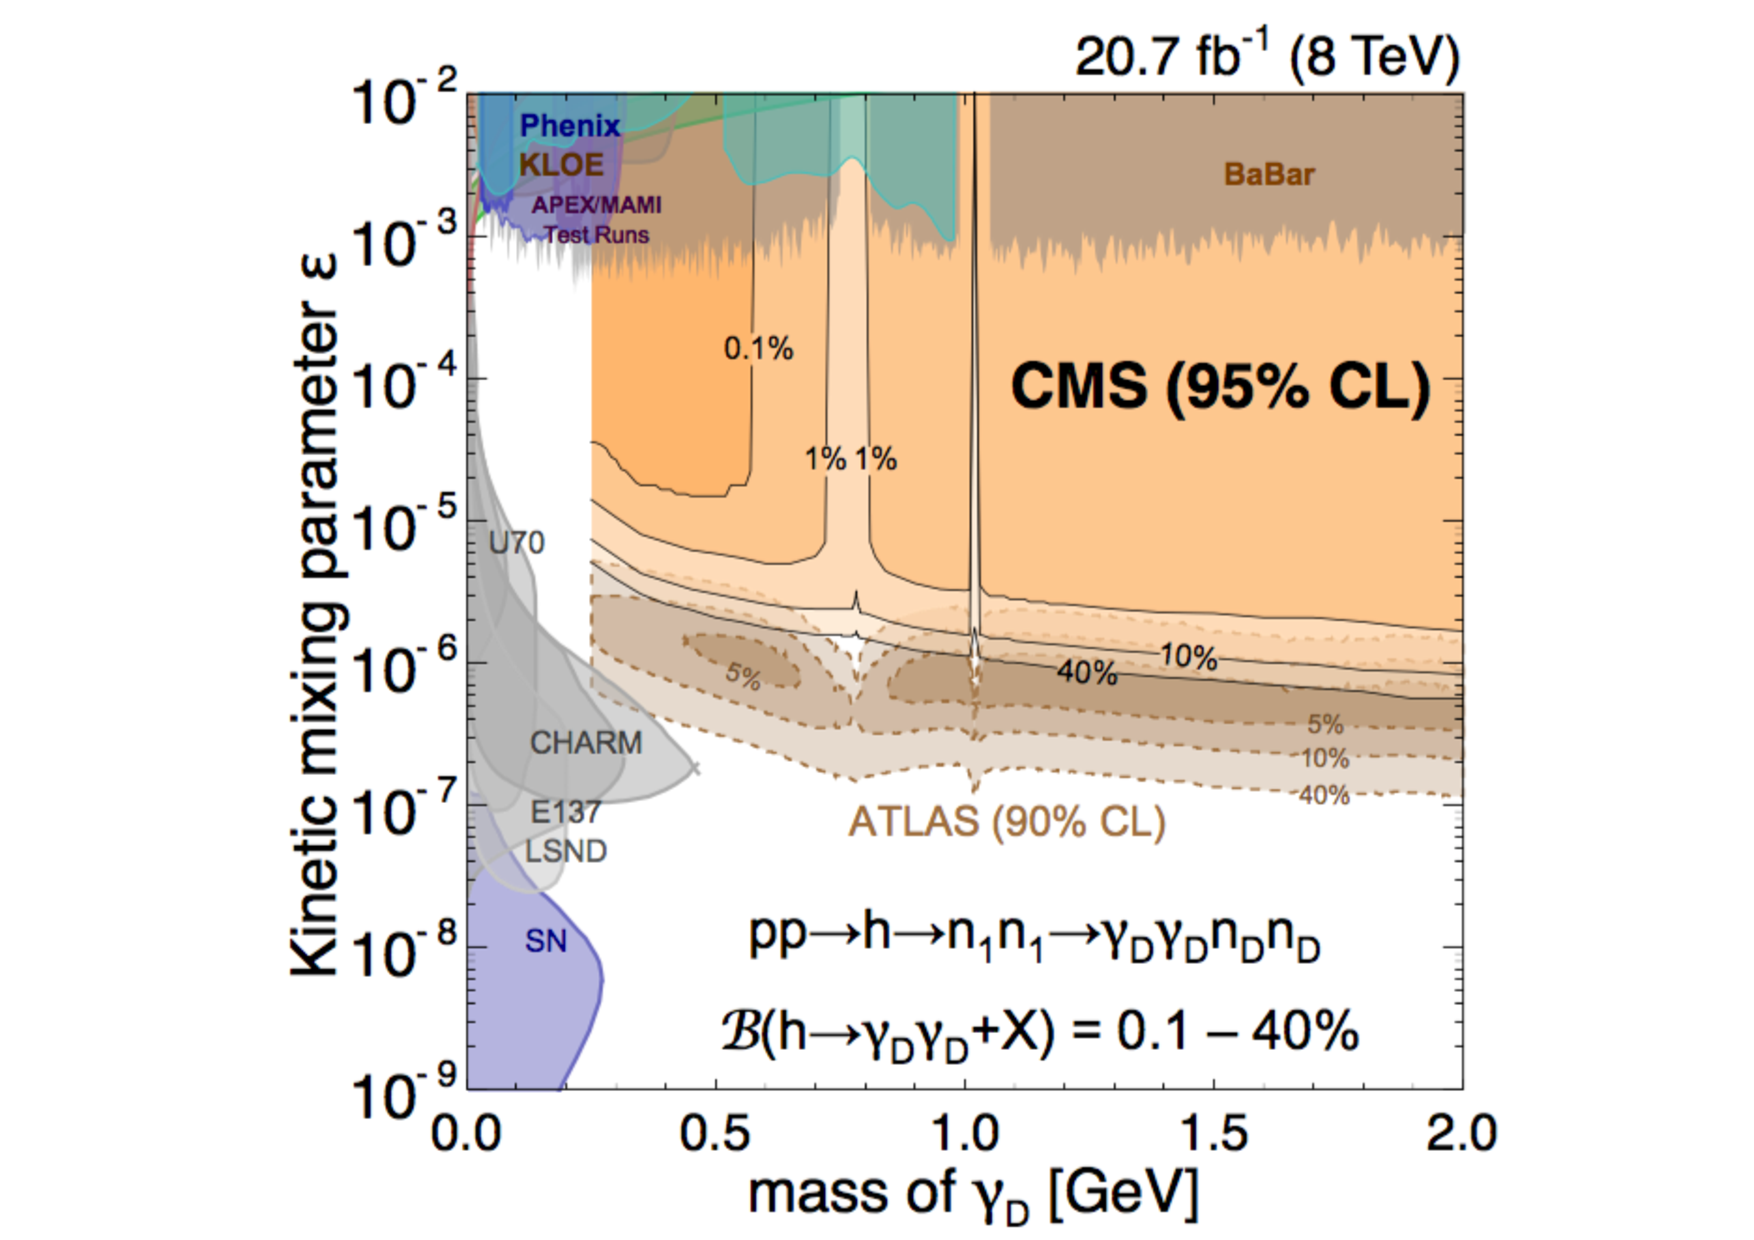
\includegraphics[width=0.7\textwidth]{plots/Limit_Eps_mass_v6.pdf}
\caption{Comparison of the lepton-jet searches at ATLAS~\cite{Aad:2014yea} and CMS~\cite{Khachatryan:2015wka} on the dark photon scenario~\cite{Falkowski:2010cm} vis-a-vis dark photon limits coming from low-energy experiments.}
  \label{fig:dark_photons_CMS_ATLAS}
\end{figure}

LHCb has a search that looks for the direct production of dark photons \cite{Aaij:2017rft}, as opposed to dark photon production in decays of the Higgs. As a result of the direct production, dark photons do not tend to be highly boosted in the transverse direction. Events are required to have a single muon with $p_{\rm T}>1.8$ GeV, or two muons with a product of transverse momenta $\gtrsim(1.5\,\,\mathrm{GeV})^2$. 
For the prompt dark photons search, events are reconstructed at trigger level so that all online reconstructed particles are recorded, while the rest of event information is discarded~\cite{Aaij:2016rxn}.
The displaced search constrains previously uncovered dark photon parameter space around masses of $\sim300$ MeV, while the prompt search constrains entirely new territory above 10 GeV.
 
The LHCb searches for displaced leptons in rare $B$ meson decays~\cite{Aaij:2015tna,Aaij:2016qsm} rely on standard techniques to identify the $B^\pm$ decay vertex and the kaons and pions in the event, and the $m(\mu^+ \mu^-)$  variable is scanned for excesses. The $X \to \mu^+ \mu^-$ vertex is not required to be displaced from the $B^\pm$ vertex, and thus the constraints apply to both prompt and long-lived particles. The analysis probes LLP masses of 214 (250) MeV $< m_X < $ 4350 (4700) MeV for the $B^0 \to K^* \mu^+ \mu^-$ ($B^+ \to K^+ X, X \to \mu^+ \mu^-$) process, with the mass range being limited by kinematics. 

To summarize, the lepton searches rely on fairly standard lepton identification, with vertex reconstruction being performed mostly offline. Searches for leptonically-decaying LLPs typically enjoy low trigger thresholds and good sensitivity to LLP production rates. A major outstanding challenge, however, are LLP decays to $\tau$ leptons, which lie at the interface between hadronic and leptonic searches. Such decays are very well motivated from the theoretical point of view, as a Higgs-like scalar would decay about 300 times more into $\tau^+ \tau^-$ if kinematically allowed, and also one could have large rates into \emph{e.g,} $\tau^+ \mu^-$.   A displaced hadronic $\tau$ is a striking object, and most likely will have few backgrounds. Hence, limits on exclusive displaced $\tau$s would be of upmost importance~\footnote{We note that if the $\tau$ originate from outside the tracker, the hadronically decaying taus are indistinguishable from other displaced hadrons. For instance, in the ATLAS Muon RoI study~\cite{Aad:2015uaa} the results are interpreted for a model with a scalar particle with Higgs-like couplings to SM fermions, which includes a branching fraction into $\tau^+ \tau^-$. However, if the $\tau$ originates from the ID, the low number of tracks associated to it (1-3) will not fulfill the requirements of the ATLAS study to having 5 or more tracks associated to a DV.}.

As the leptonic searches explicitly require opposite-sign leptons, the same-sign lepton signature (motivated from Majorana neutrinos, see the LHCb search in Section \ref{subsec:dsemilep}, or heavy, doubly charged LLPs) is currently neglected.

Lepton-jet searches currently cover only final states with at least two LLPs and some muons in the final state\footnote{The ATLAS 8~TeV search~\cite{Aad:2014yea} included a search channel with two electron-only lepton-jets, but the performance was poor and it was excluded from the final result.}, and the same statement currently applies to both the LHCb searches for dark photons~\cite{Aaij:2016rxn,Aaij:2017rft} 
 and for LLPs produced in $B$-meson decays. It would be beneficial to have additional searches with one lepton-jet or low-mass, leptonically-decaying LLP (which are motivated in hidden sectors and Majorana neutrinos, for example in Refs.~\cite{Izaguirre:2015pga,Izaguirre:2015zva}). In addition, the status of coverage in the intermediate mass-transition region between ``standard" displaced lepton pairs and lepton-jets is unclear, and may potentially harbor a gap.  

 Heavy Neutral Leptons (HNL) are ubiquitious in New Physics models. They constitute an  important physics case that leads to multi-lepton displaced signatures from $W$ decays, with nice prospects at ATLAS and CMS~(see e.g.~ \cite{Izaguirre2015,Nemevsek:2018bbt,Cottin:2018kmq}). While previous searches were not sensitive to this scenario due to either high-$p_T$ requirements or the requirement of two DVs in the same event, the presence of a prompt lepton from the $W$ allows to relax on these in a dedicated analysis (triggering on the prompt lepton was studied recently in~\cite{Cottin:2018kmq}.)~\footnote{Note that the displaced large transverse impact parameter $e$-$\mu$ CMS search~\cite{CMS-PAS-EXO-16-022} fails to cover this scenario due to the aforementioned lepton veto, which kills the tri-lepton signals discussed in Ref.~\cite{Izaguirre2015}. }. 
The identification of two leptons from the vertex is a powerful discriminant against backgrounds from meta-stable particle decays and hadronic interactions in material. This permits a better exploration of the lower HNL mass range ($3-6$~GeV) than in the semi-leptonic channel (see Section~\ref{subsec:dsemilep}) despite the lower branching ratio. It should be noted that the ambition is to probe mixing to all three neutrino flavors, requiring the capability to reconstruct displaced leptons of all flavors, including taus. 

\subsection{Semi-Leptonic decays}
\label{subsec:dsemilep}

As semi-leptonic signatures include aspects of both hadronic and leptonic LLP decays, many of the previously discussed searches can partially cover these cases, and some do so explicitly. For instance, the ATLAS search for electrons and muons accompanied by tracks~\cite{Aad:2015rba}, the inclusive CMS search for DVs~\cite{CMS:2017oor} (there is an specific model interpretation called $B$-lepton addressing precisely this channel), and the large impact parameter $e-\mu$ pair by CMS~\cite{CMS-PAS-EXO-16-022} are all inclusive with respect to other hadrons produced in the LLP decay, provided the leptons are sufficiently isolated~\footnote{Note that the lepton isolation affects most of the semi-leptonic searches.}. In addition, LHCb has dedicated searches for semi-leptonically decaying  LLPs~\cite{Aaij:2016xmb} and semi-leptonic decays of long-lived Majorana neutrinos coming from $B^{-}$ mesons~\cite{Aaij:2014aba}.   The two CMS searches \cite{CMS:2017oor,CMS-PAS-EXO-16-022} need no further explanation for how they cover semi-leptonic LLPs, but we now describe the rest of these searches in some detail.    

The ATLAS search for a vertex with a lepton accompanied by tracks \cite{Aad:2015rba} uses the same trigger as the dilepton vertex search described in Sec.~\ref{subsec:dleptons}. The DV is required to have a lepton as well as at least four additional displaced tracks associated with it, and the invariant mass of the tracks must exceed 10 GeV.  Thus, the search in principle can have sensitivity down to masses $\gtrsim10$ GeV, although the very high $\pT$ threshold for the displaced electron(photon)/muon typically limits sensitivity for low-mass LLPs: the vertex must contain a muon with $\pT > 55$~GeV or an electron with $\pT > 125$~GeV.

The LHCb search for semi-leptonic LLP decays selects events with a muon trigger, then requires a DV offline~\cite{Aaij:2016xmb}. The results are interpreted in terms of four distinctive topologies: single LLP production in association with a new particle, and double LLP pair production either from Higgs decays or via squark pair production.  Material regions are vetoed, leaving heavy flavor produced either directly or from $W/Z$ decays as the dominant background. The signal discrimination is obtained from a multivariate analysis based on the muon $\pT$ and impact parameter, and subsequently the search is optimized based on the LLP reconstructed mass and the muon isolation. This study is sensitive to lifetimes between 1.5 and 30 mm, as can be seen in Figure~\ref{fig:lhcbsemileptonic}. 

\begin{figure}[htb]
\centering
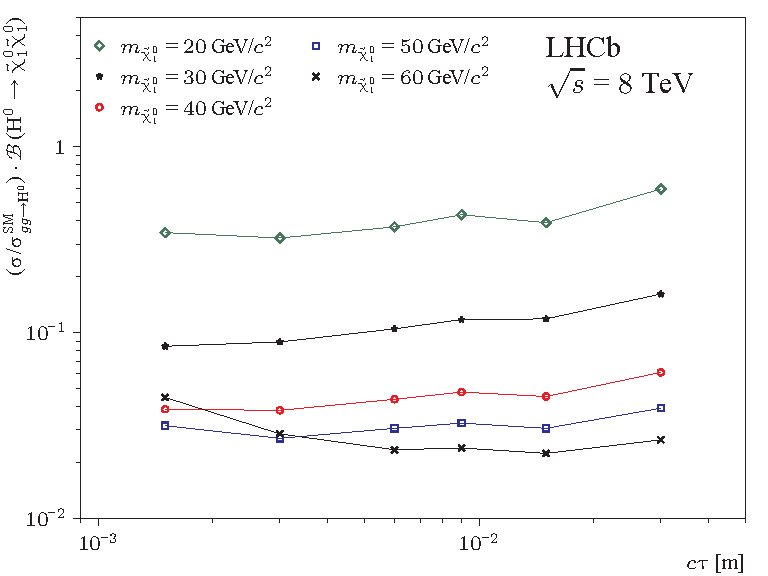
\includegraphics[width=0.9\textwidth]{plots/PAPER-2016-047_sup1.pdf}
\caption{LHCb reach for displaced semi-leptonic decays. Taken from ref~\cite{Aaij:2016xmb}.}
\label{fig:lhcbsemileptonic}
\end{figure}

The LHCb search~\cite{Aaij:2014aba} looks for Majorana neutrinos, $N$, produced in leptonic $B$ decays, $B^\pm\rightarrow \mu^\pm N$, followed by the  decay $N\rightarrow \mu^\pm\pi^\mp$, whether prompt or at a DV~\footnote{Much care is required in interpreting the results of the search on a model with a Majorana neutrino, as the original theory interpretation is problematic. See~\cite{Shuve:2016muy} for un updated analysis and revised limit.}.
 A same-sign muon requirement greatly reduces backgrounds to the search. The sensitivity of the search is limited by the restriction to muons in the final state (so models that predominantly decay to $e$ or $\tau$ are not constrained), as well as the same-sign lepton requirement to only lepton-number-violating processes. More inclusive searches looking for additional $N$ production modes \cite{Gorbunov:2007ak} or searches targeting decays of heavier mesons like $B_c$ \cite{Milanes:2016rzr} could also improve the sensitivity to semi-leptonically decaying LLPs. 

When considering the application of inclusive, hadronic or leptonic searches to semileptonic LLP decays, it is important to understand how the simultaneous presence of leptons and jets in the signal can degrade the sensitivity. For instance, prompt jet searches explicitly veto non-standard jets. Lepton isolation criteria can severely reduce the signal acceptance for a highly-boosted LLP decaying into a lepton and a jet, and they might also veto extra tracks in the events. Thus,  boosted semi-leptonic decays (as might be found in the displaced decay of a low-mass right-handed neutrino produced via $W$ decay) may not be covered by existing searches. 
Another important issue is that the lepton-jet studies express their results in terms of specific dark photon models~\footnote{Recall that the lepton-jet studies also consider the $\gamma_D \to \pi^+ \pi^-$ decay mode.}, which makes it complicated to apply the results to other models. We refer the reader to Sec.~\ref{sec:reint} for a further discussion of this topic.

The signature of HNLs from $W$ decays with displaced semi-leptonic HNL decays is an important item on the search agenda of ATLAS, CMS and LHCb~\cite{Helo2014,Izaguirre2015,Mermod2017,Antusch2017,Nemevsek:2018bbt,Cottin:2018kmq}. The semi-leptonic channel has the highest branching ratio (about 50\% in the relevant mass range~\cite{Gronau1984}) and offers the best discovery prospects at LHC experiments for HNL masses up to 30~GeV as long as a DV mass cut of around 6~GeV is made to mitigate backgrounds from B-mesons, $m_B \sim 5 GeV$. This $6-30$~GeV mass range corresponds to a non-perturbative regime for the hadronisation of the HNL decay products. As the number of charged hadrons significantly affects the DV reconstruction efficiency, the validation of event generator outputs for this process is an important issue currently being addressed by the community (see e.g.~\cite{Cottin:2018kmq}). The ability of LHCb to trigger directly on the HNL decay products and better reconstruct displaced tracks can in some cases compensate for its lower acceptance and luminosity, as exemplified by a recent search for DVs made one muon and several tracks~\cite{LHCb2017,Antusch2017}. This possibly enables LHCb to better probe the more challenging tau channel. Fig.~\ref{fig:HNLsensitivity} shows the overall expected reach of LHC searches in the HNL coupling strength (muon channel) versus mass plane, using assumptions detailed in Ref.~\cite{Mermod2017}, similar to those in Refs.~\cite{Helo2014,Izaguirre2015}. An interesting aspect of the LHC HNL search programme is that backgrounds can be mitigated at high luminosities using the DV feature, making this signature particularly attractive at the HL-LHC. 

The sensitivity of LHC experiments to HNLs is complementary to that of fixed-target experiments which can probe lower couplings thanks to high-intensity beams albeit at lower mass ranges (HNLs from $c$ and $b$ decays). The CERN SPS provides great opportunities with the running NA62 experiment~\cite{NA622017a} and the planned SHiP experiment~\cite{SHiP2015}, which comprise a vacuum decay vessel and spectrometer tracker downstream of the target to reconstruct vertices of long-lived neutral particles~\footnote{The proposed detector FASER would also the capability to reconstruct such vertices~\cite{Kling:2018wct}.}. These are unbeatable for HNL masses up to 2~GeV, where they probe a region of the parameter space favoured in models which explain at once neutrino masses, matter-antimatter asymmetry and dark matter~\cite{Asaka2005b,Canetti2013b,Mermod2017b} (see Fig.~\ref{fig:HNLsensitivity}).

\begin{figure}[t]
\centering
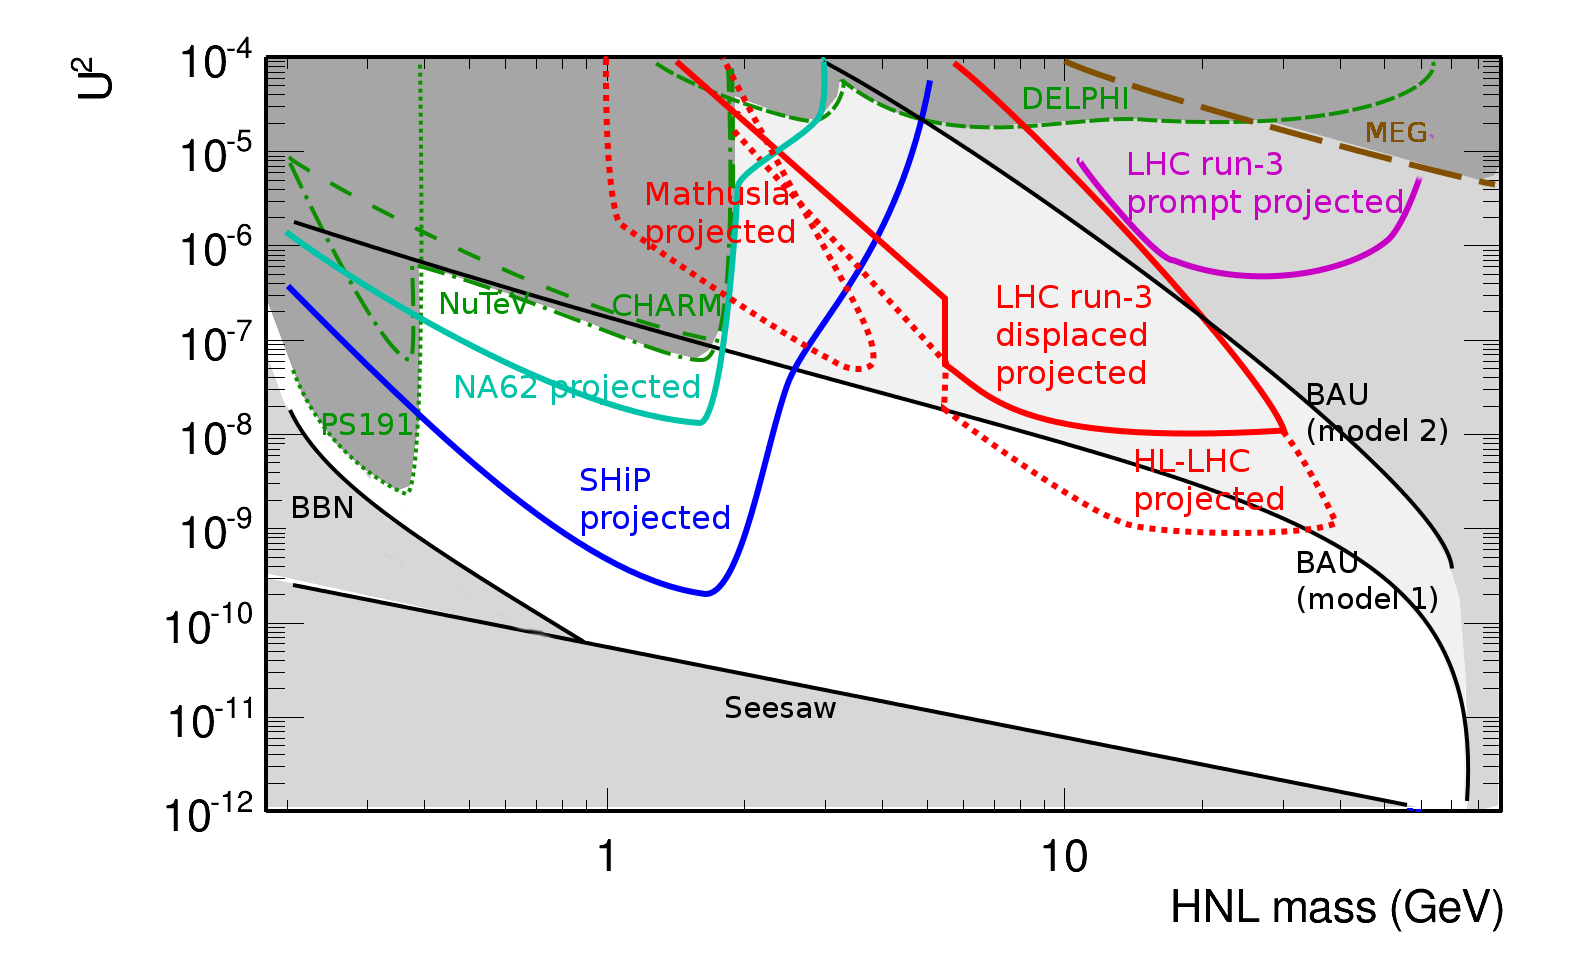
\includegraphics[width=0.99\linewidth]{figures/BigPicture.png}
\caption{Summary of projected experimental sensitivities to HNLs in various experiments, in the coupling strength ($U^2$ for dominant mixing to $\nu_\mu$) vs. mass plane. The projections labelled ``LHC run-3'' and ``HL-LHC'' are for HNLs in $W$ decays in general-purpose experiments, and the one labelled ``Mathusla'' assumes the full HL-LHC Mathusla dataset. Prospects at near-future proton beam-dump experiments are also shown for NA62~\cite{Lanfranchi2017} and SHiP~\cite{SHiP2015}. Direct~\cite{Bernardi1988,CHARM1986,NuTeV1999,Delphi1997,CMS2015b} and indirect~\cite{MEG2013,Antusch2015} limits are indicated as dashed green and brown lines respectively. The lines labelled ``Seesaw'' and ``BBN'' show lower theoretical constraints from the observed neutrino masses (normal hierarchy) and primordial nucleosynthesis, respectively~\cite{Canetti2013b}. The lines labelled ``BAU'' are upper theoretical constraints from two different models accounting for baryon asymmetry in the Universe: model 1 requires the lightest HNL to be the dark matter~\cite{Canetti2013b}, while model 2 allows for all three HNLs to participate in leptogenesis~\cite{Canetti2014}. }
\label{fig:HNLsensitivity}
\end{figure}

\subsection{Photonic decays}
\label{subsec:dphotons}

There are two ways in which photons coming from LLP decays do not resemble standard photons. First, they can not be traced back to the PV, thus giving rise to \emph{non-pointing} photons. Second, they can arrive at the electromagnetic calorimeter at a slight different time than expected, referred to as \emph{delayed} photons.  We note that both these kinds of unusual photons can be vetoed when considering prompt photons, and thus the recasting of prompt searches typically provides weaker bounds on LLP scenarios.  ATLAS has a search for non-standard photons~\cite{Aad:2014gfa} using the full 8~TeV dataset, which supersedes the 7~TeV analysis~\cite{Aad:2013oua}, while in CMS there are studies for delayed photons in the ECAL~\cite{CMS:2015sjc} and for non-pointing photons detected via their conversion to $e^+ e^-$ pairs~\cite{CMS:2015gga}. The underlying topology in all these models is the neutralino decay into a gravitino and a photon ($\chi^0_1 \to \gamma \tilde{G}$), ubiquitous in gauge-mediated supersymmetry breaking (GMSB) scenarios~\cite{Dine:1994vc,Giudice:1998bp}. Hence all these studies require to have large $\metm$ in the final state.

The ATLAS study benefits from the capability of the liquid-argon electromagnetic calorimeters to measure the flight direction and the time-of-flight of photons. Resolutions on $\Delta z_\gamma$, the separation between the PV of the event and the extrapolated origin of the photon, and $|\Delta t_\gamma|$, difference of the arrival time of the photon with respect to the prompt case, are as low as 15~mm and 0.25~ns, respectively. The trigger demands two photons within $|\eta| < 2.5$, with transverse energies $E_T$ of 35 and 25 GeV.  
In addition, to guarantee the event comes from a proton--proton collision, a PV with 5 or more tracks with $\pT > 0.4$ GeV is requested.
The offline selection requires two photons with $E_T >$ 50 GeV and $|\eta| < 2.3$, not in the barrel-endcap transition region ($1.37 < |\eta| < 1.52$), at least one of them in the barrel ($|\eta| < 1.37$) and with less than 4 GeV energy deposit in the calorimeter in a cone of $\Delta R =0.4$ around them (\emph{isolation}). In addition, the events are binned in $\metm:$ the $\metm < 20$ GeV bin contains the prompt backgrounds, the 25 GeV $< \metm < 75$ GeV bin is used as the control region, and finally the signal analysis is performed in the $\metm > 75$ GeV bin. This study covers lifetimes from 0.25 to 100~ns in the GMSB framework, the lower limit being a hard cut-off imposed experimentally, as the similarity between background and signal samples in that region makes discrimination rather difficult. The excluded signal rates in this range of lifetimes vary between 0.8 and 150 fb, with the best-constrained value obtained for $\tau \sim$ 2 ns.
 
The CMS study of delayed photons~\cite{CMS:2015sjc} follows a similar approach to ATLAS. The main difference is that it demands only one photon with $\pT > 80$ GeV, but in addition two jets are required. Furthermore, in addition to \met, the vector sum of \met and $E_T^\gamma$, which is denoted $E_{T~{\rm no }\gamma}^{\rm miss}$, is used for background discrimination. (Non)-collisional backgrounds have small (large) \met and  large (small) $E_{T~{\rm no }\gamma}^{\rm miss}$, while for the signal events both variables are large, hence they are both requested to be larger than 60 GeV. The time resolution is 0.372~ns, slightly worse than in the optimal scenario of the ATLAS search. Their reach in lifetimes lies in the 2--30~ns range, excluding signal rates of 10--30 fb.
 
The CMS study of non-pointing photons~\cite{CMS:2015gga} relies on conversion to $e^+ e^-$ pairs. It requires two photons, two additional jets, and $\metm > 60$ GeV. The photon trajectory is obtained from the conversion vertex as the line segment along the momenta of the $e^+ e^-$ track pair, and the impact parameter, $|d_{XY}|$, is defined as the closest distance between the photon and the beam axis, can be determined within approximately 1 mm.
A comparison of the reach of these 8 TeV studies, as well as those using the 7 TeV dataset, can be found in Fig.~\ref{fig:gaga}.
 
%%%%%%%%%%%%%%%%%%%%%%%%%%%%%%%%%%%%%%%%%%%%%%%%
\begin{figure}[htb]
\centering
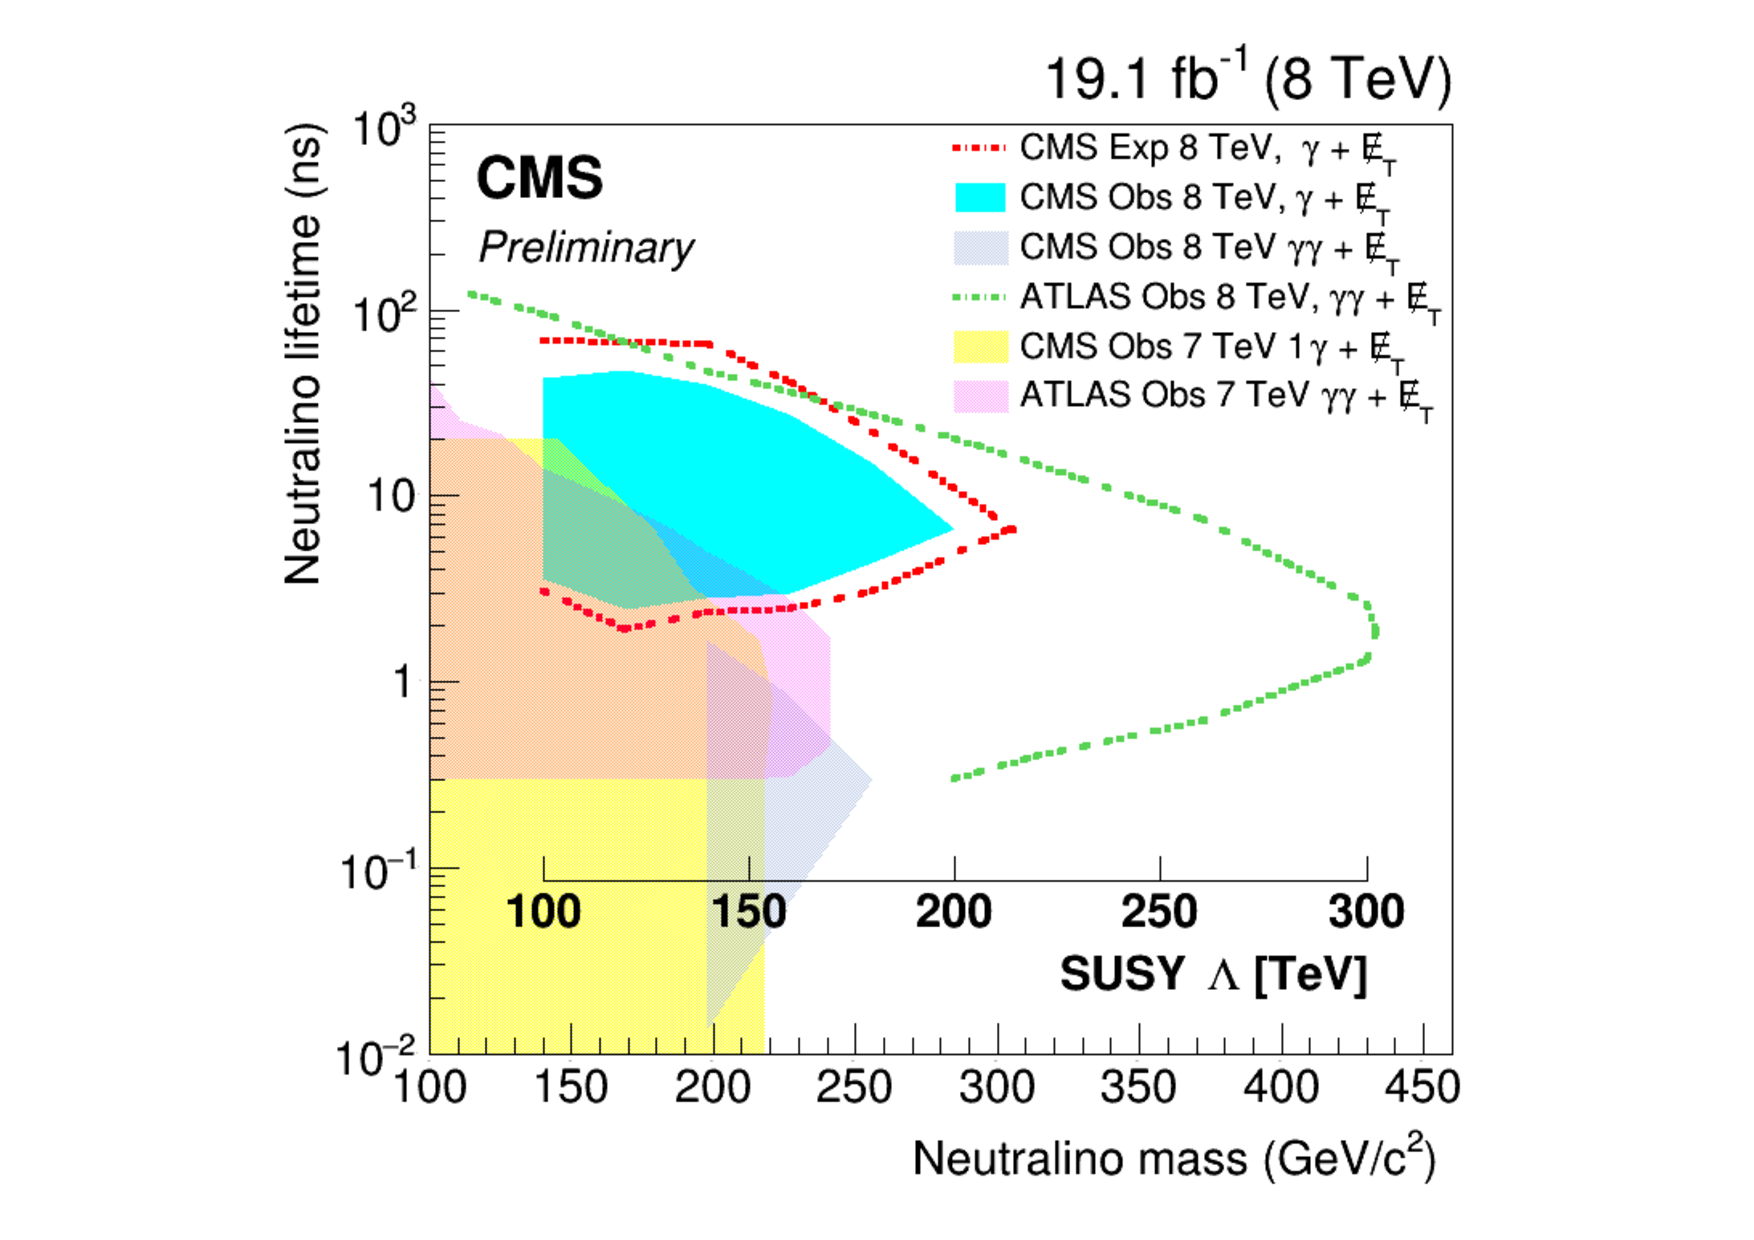
\includegraphics[width=0.7\textwidth]{plots/CMS-PAS-EXO-12-035_Figure_016-a.pdf}
\caption{Summary of the $\gamma + \metm$ searches from ATLAS and CMS, displayed assuming the same GMSB model. Taken from reference~\cite{CMS:2015sjc}. 
}
  \label{fig:gaga}
\end{figure}
%%%%%%%%%%%%%%%%%%%%%%%%%%%%%%%%%%%%%%%%%%%%%%%
 
The gaps in these studies are straightforward to identify. The requirement of large $\metm$ is due to the fact that all of these studies have an underlying theoretical picture of neutralinos decaying into gravitinos and photons, motivated from GMSB scenarios.   Hence, these searches do not cover cases without the presence of missing energy, including LLPs that decay to $\gamma \gamma$, $l \gamma$ or $j \gamma$, although either mis-measurement of jets or the photon decay geometry could fake large missing energy to provide moderate constraints. With the exception of the CMS study~\cite{CMS:2015sjc} which requires two additional hard jets, all of these analyses require two displaced photons.  A single displaced photon signature can occur in motivated models:~it can easily arise, for example, from a very slightly mixed electroweak triplet and singletm belonging to the SUSY Simplified Model category from Sec.~\ref{sec:simplifiedmodel}. Furthermore, as discussed in section~\ref{subsec:djets}, a single LLP in the detector can also arise for very large lifetimes of neutral LLPs, which limits the reach at longer lifetimes.

\subsection{Other exotic long-lived signatures}
\label{subsec:funnytracks}

In this section we present the analyses that are based on exploiting properties of other exotic long-lived signatures, such as non-standard tracks.  We summarize in detail the existing searches for heavy stable charged particles (HSCP), disappearing tracks (DT), stopped particles (SP) and monopoles, and describe  existing ideas on how to look for quirks and SIMPs (Strongly Interacting Massive Particles).

\subsubsection{Heavy Stable Charged Particles (HSCP)} 
\label{subsec:ExpHSCP}

The search for HSCPs at CMS~\cite{Chatrchyan:2013oca,CMS:2016ybj} and ATLAS~\cite{ATLAS:2014fka,Aaboud:2016uth} rely on two key properties. First, particles that are massive and/or electrically charged with $Q \ne \pm e$ have a  characteristic ionization energy loss ($dE/dx$) distinctively different than SM particles. 
%This property can be measured in the tracker.
Second, HSCPs are typically heavy and move with a speed smaller than the speed of light, $\beta = v/c < 1$. Thus, compared to a particle with $\beta \approx 1$, they require a longer time-of-flight (TOF) to reach the outermost components of the detector (calorimeters and muon chambers).  Interactions of the HSCP with the material in the detector can change the electric charge of the HSCP and they occur randomly. Hence both CMS and ATLAS perform separate \emph{tracker-only} and \emph{tracker + TOF} studies in the language of CMS~\footnote{ATLAS measures $\beta \gamma$ from $dE/dX$ and $\beta$ from time-of-flight and extracts an independent mass, $m_{\beta}$ and $m_{\beta \gamma}$, from each measurement~\cite{Aad:2011hz,ATLAS:2014fka,Aaboud:2016uth}}. The event selection relies on standard single-muon or large-missing-energy triggers. The offline selection relies on identifying the signal events from quality requirements on the tracks using discriminator variables built from track observables. 

The theoretical interpretation of a signal or limit depends on whether the HSCP carries both color and electroweak charges. If it carries a color charge, the default benchmarks correspond to $R$-hadrons, namely HSCPs that hadronize with SM particles via the strong force (e.g gluino--gluon, quark--squark states). In the absence of a color charge, the signal is exemplified by long-lived sleptons in the context of gauge-mediated and anomaly-mediated SUSY breaking. Both ATLAS~\cite{ATLAS:2014fka} and CMS~\cite{CMS:2016ybj} studies employ these two scenarios\footnote{The ATLAS R-hadron searches using the 13 TeV dataset have recently been presented in reference~\cite{Aaboud:2016uth}. }.
Finally, CMS also looks for HSCPs coupling only to hypercharge (and hence possessing only couplings to $\gamma$ and Z), while ATLAS has a search inspired by electroweakinos in SUSY:~it considers the associated production of a neutral and an electrically charged LLP (chargino--neutralino), and thus only one HSCP plus missing energy are required.

The HSCP search conducted by LHCb~\cite{Aaij:2015ica} is slightly different.
Instead of exploiting $dE/dx$ and time-of-flight, they use the lack of radiation in the ring imaging Cherenkov detector (RICH). Events are required to pass a high-\pT single-muon trigger ($\pT(\mu) > 15$ GeV). Two opposite sign muons are then required, each with \pT above 50 GeV and an invariant di-muon mass above 100 GeV, to suppress muons coming from Drell-Yan production, the main background for this search. In addition, particles must have $\beta > 0.8$, set by the efficiency of the muon chambers to reconstruct slow particles. As electrons and hadrons interact more with the calorimeter than an HSCP, a deposit in the calorimeter of less than 1\% of the momentum of the particle is required.  The results are interpreted in the context of stau pair production.

To summarize, these searches are robust, though, without any dedicated trigger, the efficiency starts to decrease with $\beta$ values below 0.8. It would be worth exploring ideas to overcome this difficulty. The small number of signal events that would be produced for HSCPs above current limits render the sensitivity highly dependent on the understanding of the background and the control of the systematics.

%To summarize, these searches are robust, but the trigger efficiency drops with decreasing $\beta$. It would be worth exploring trigger strategies to probe such values of $\beta \lesssim 0.6 - - 0.8$.
%%$\beta \lesssim 0.6 - - 0.8$.
%%present no obvious weak points. Standard triggers and tracking algorithms are used, and the analysis methods are well-understood and have been extensively validated against data. While the HSCP strategies are robust, 
%%we encourage the experimental collaborations to continue pursuing improvements for these searches. In particular it would be worth exploring ideas to probe particles with $\beta < 0.8$, which at the moment is an inherent hardware limitation. 
%The small number of signal events that would be produced for HSCPs above current limits render the sensitivity highly dependent on the understanding of the background and the control of the systematics.

\subsubsection{Disappearing tracks (DT)} 

Massive charged particles traveling in the detector can decay to a lighter, almost mass degenerate neutral state, emitting a SM charged particle (typically a pion or a muon). While at first glance a small mass gap na\"ively seems like a hallmark of tuning, near degeneracies often occur naturally as a result of a symmetry. In fact, electroweak symmetry generically leads to small mass splittings $\Delta$ between components of a single electroweak multiplet. For example, ${\cal O} (100 $ MeV) splittings arise between the different components of an electroweak multiplet~\cite{Thomas:1998wy,Cirelli:2005uq} due to EW gauge boson loops~\footnote{For a single fermionic multiplet, the splitting can only be altered by higher-dimensional operators, and thus it is harder to vary $\Delta $ from the 1-loop EW value. For other cases, such as mixing with additional particles, the actual splitting can differ greatly than this 1-loop EW value.}. If the SM particle is sufficiently soft it can not be reconstructed, and then a charged track seems to vanish: this is thus referred to as a disappearing track~\footnote{If the charged particle could be reconstructed this case is often referred to as \emph{kinked track}.  However, as the kinked portion has a very large impact parameter, without a serious attempt to capture the kink these tracks too simply disappear.}.  The actual lifetime of the charged particle is highly sensitive to the precise value of the mass splitting. For instance, the well studied cases of a fermionic doublet with $Y=1/2$ and a fermionic triplet with $Y=0$, reminiscent of a Higgsino and Wino in supersymmetry, respectively, have mass splittings of $\Delta = 355$ and 166 MeV up to small corrections, but the corresponding $c \tau$ differ by almost an order of magnitude: 6.6 mm versus  5.5 cm\footnote{While these values set a concrete physics target, we stress again that the mass splitting can be arbitrary in other corners of the BSM parameter space (even within SUSY). For instance,  $\tilde{\tau} \to \tau \tilde{\nu}$ (where the stau and sneutrino masses are free independent parameters) or for scalar particles (e.g: $H^+ \to \mu^+ H^0$), where the mass splitting and the overall mass scalar are set by arbitrary quartic couplings.}. This is because the lifetime, $c\tau$, depends on the third power of the mass splitting in these scenarios \cite{Thomas:1998wy,Cirelli:2005uq}. 

Before 2017, both ATLAS~\cite{Aad:2013yna} and CMS~\cite{CMS:2014gxa} required a track to travel about 30 cm in order to be reconstructed, giving good coverage of the Wino scenario. These 30 cm correspond to four hits at ATLAS, three in the pixel layers plus one in the silicon tracker, and to seven hits in the pixel and trackers of CMS. The search uses a trigger requiring an ISR jet against which the charged particle recoils, along with the presence of large missing energy. The disappearing track is reconstructed offline and needs to fulfil a few quality criteria (isolation, \pT threshold, etc). A phenomenological study~\cite{Mahbubani:2017gjh} had shown that reducing the distance from 30 to 10 cm would give coverage to the elusive Higgsino scenario, moving the expected reach up to 400 GeV, trumping over the expected mono-jet reach of 250 GeV~\cite{Schwaller:2013baa,Low:2014cba,Barducci:2015ffa}. Later ATLAS presented a study~\cite{ATLAS-CONF-2017-017} using 13 TeV data and exploiting the presence of a new innermost pixel layer (IBL). This addition allows for all four hits to be in the pixel, with the outermost pixel layer now at 12.25 cm,  granting sensitivity to lower values of $c \tau$. The summary for disappearing tracks at ATLAS for the Wino case can be seen in the left panel of Figure~\ref{fig:ewkinosearches}, while in the right panel we show the constraints for Higgsinos from reference~\cite{Mahbubani:2017gjh}.

\begin{figure}[htb]
\centering
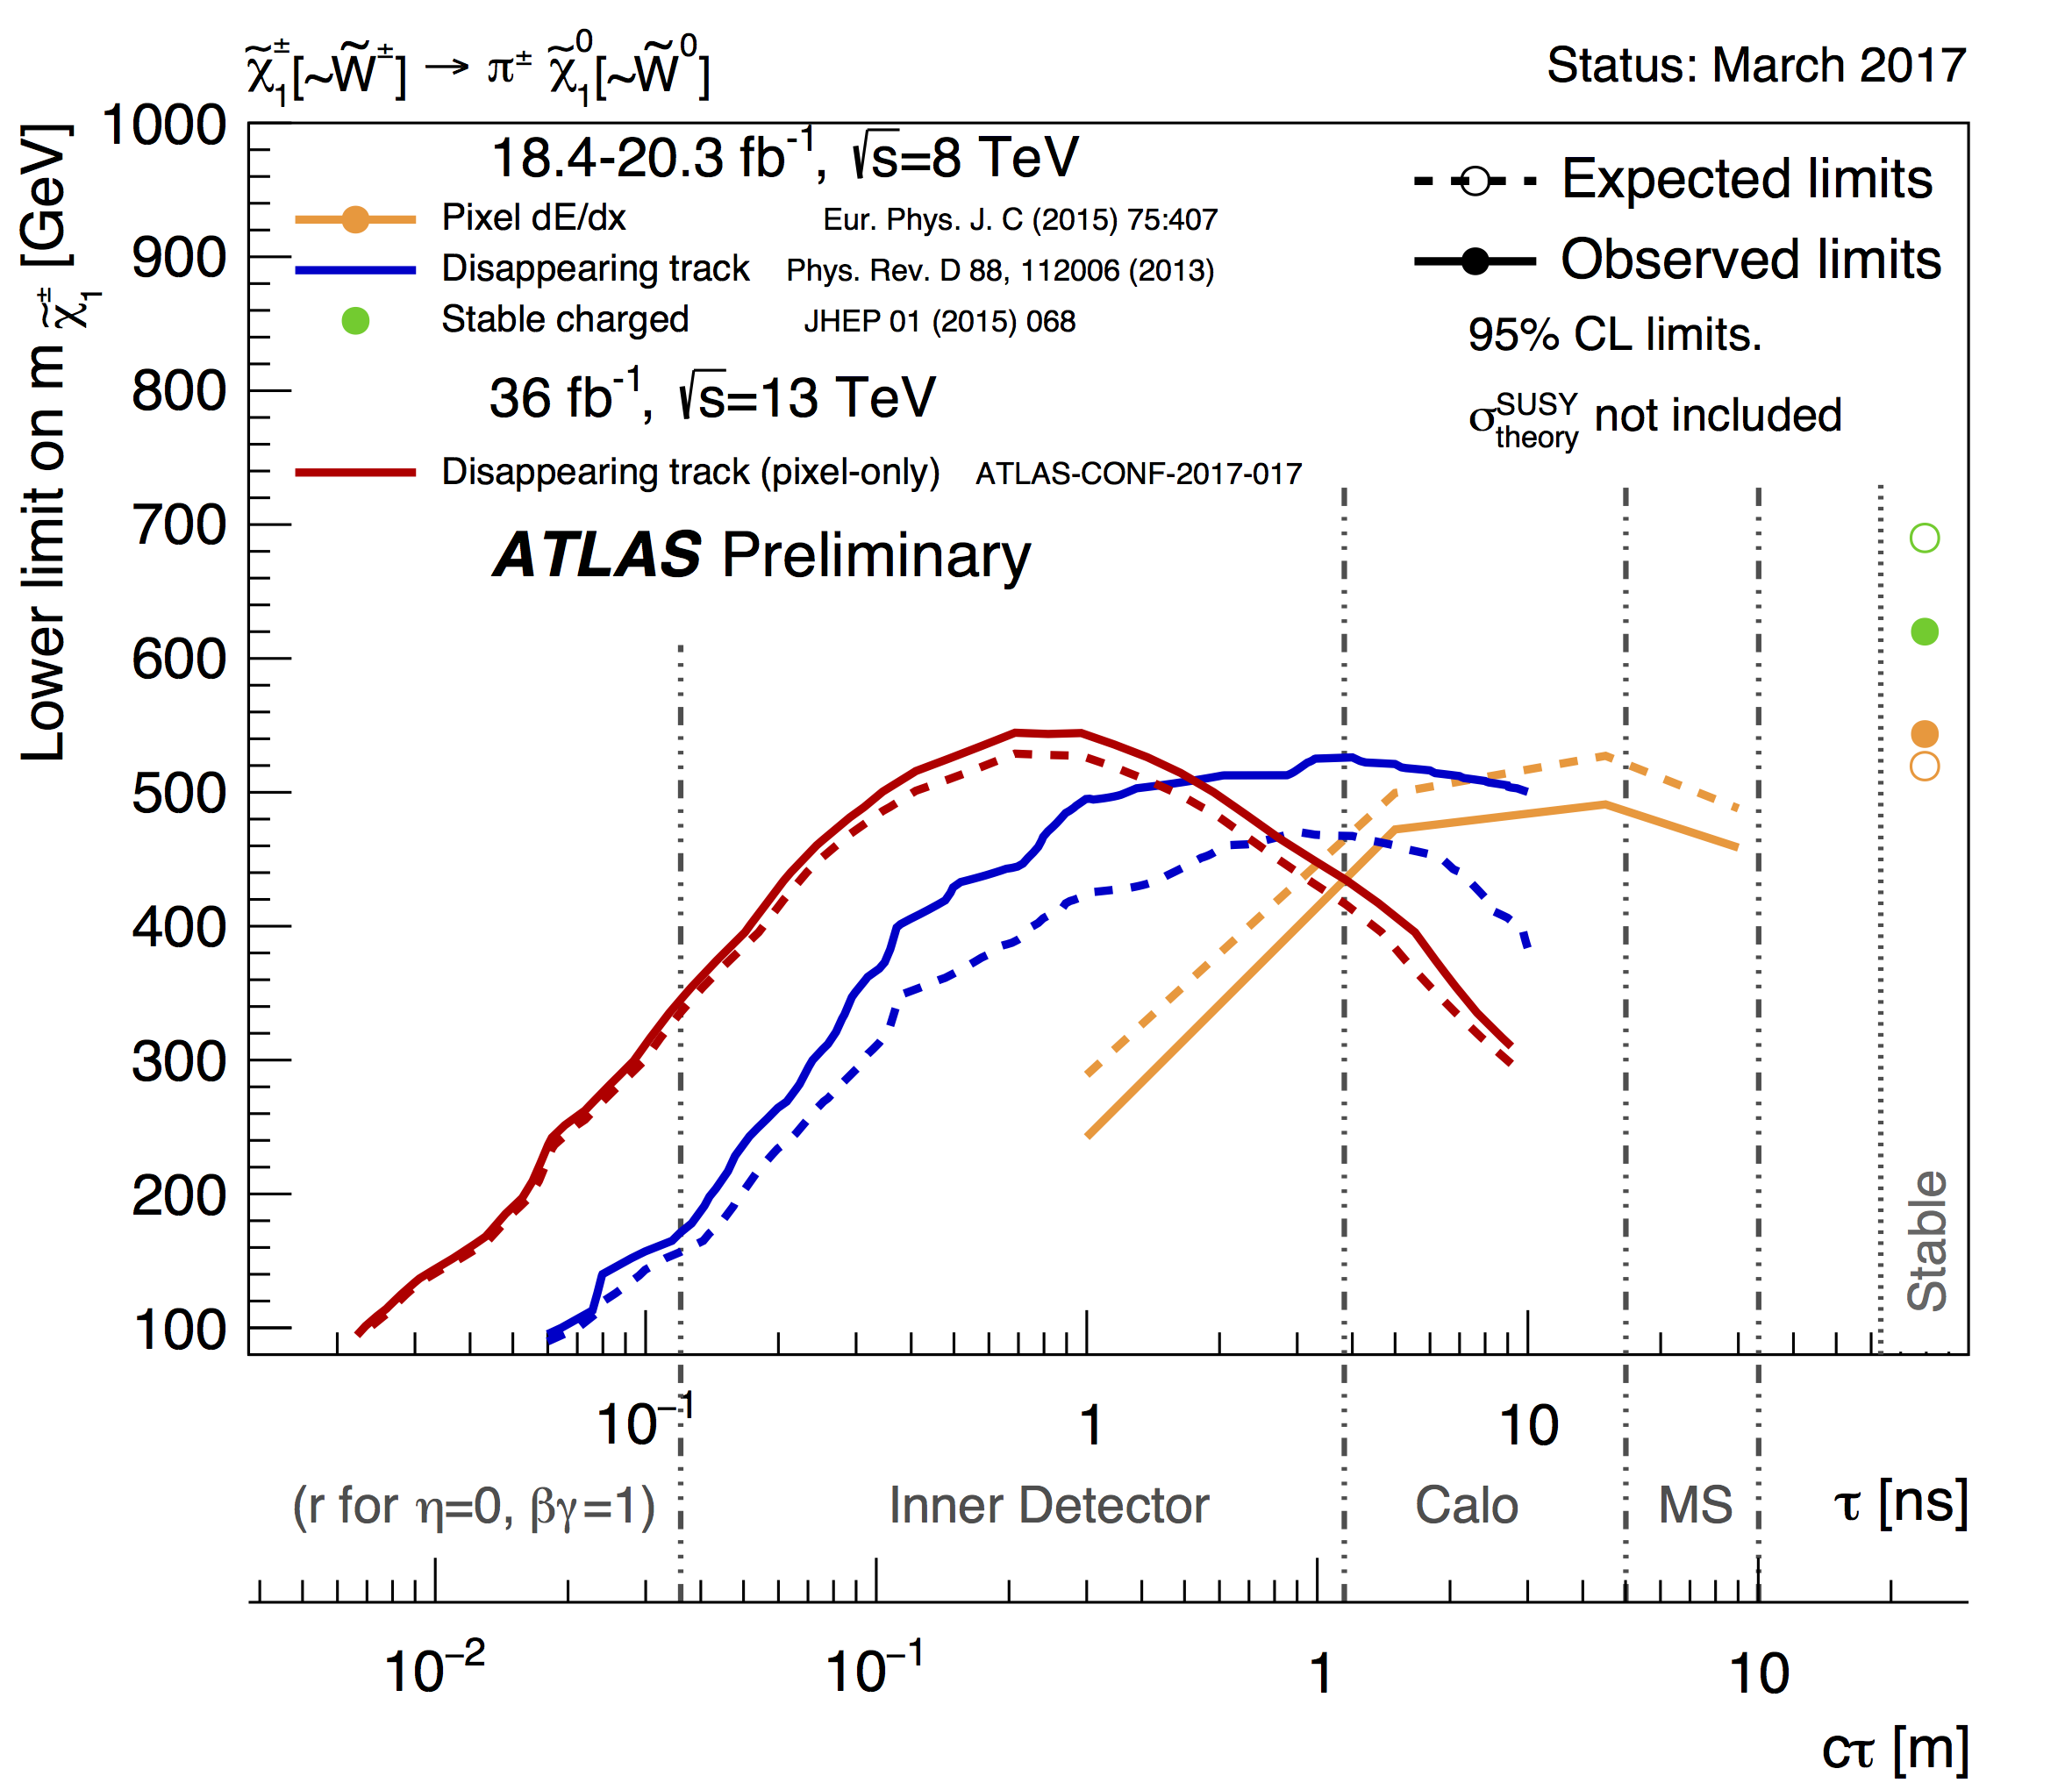
\includegraphics[width=0.44\textwidth]{plots/ATLAS_SUSY_LLPChargino.png}
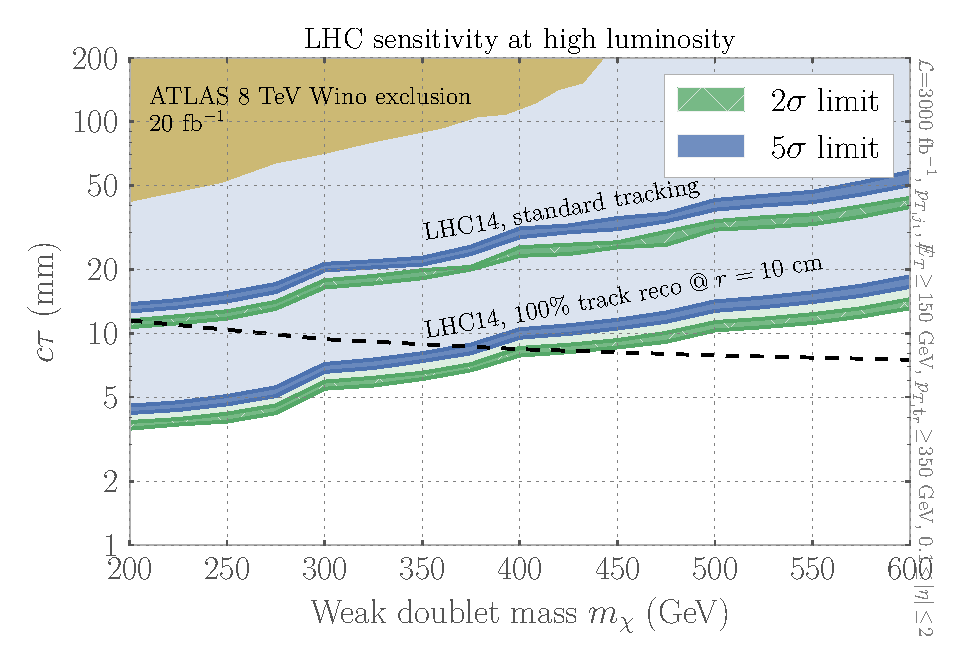
\includegraphics[width=0.54\textwidth]{plots/Higgsino_Significance14}
\caption{Summary of the status of Wino searches in ATLAS (left panel) and HL-LHC expected constraints on the Higgsino scenario (right). Taken from~\cite{ATLAS:summary} and ~\cite{Mahbubani:2017gjh} respectively.}
  \label{fig:ewkinosearches}
\end{figure}

At LHCb the prospects for a disappearing track analysis with the present detector are poor. Currently, the momentum of the track can only be measured if the particle passes through the Tracker Turicensis (TT), which is about 3~m away from the IP. Particles decaying in the VELO or RICH1 system will not leave a fully-measurable track and will be swamped in a background of SM processes such as kaon decays, which would give a similar signature in the detector components before the magnet. Detector improvements such as additional magnets, better particle identification (PID) at low momentum and additional layers might lead to some sensitivity for ${\cal O}$(cm) lived tracks.

%If the detector were improved (by e.g: adding station magnets, better PID at \textcolor{red}{To be completed.}

To summarize, the searches for disappearing tracks present a few drawbacks. Using an ISR-jet trigger means a price is paid in terms of signal sensitivity: reference~\cite{Mahbubani:2017gjh} has shown that significantly lowering the \pT threshold of the jet (or directly triggering on the momentum of the disappearing track~\footnote{While currently there are some proposals to trigger on tracks~\cite{Gershtein:2017workshop}, those only apply to standard tracks. In particular, the new fast track reconstruction (FTK) system at ATLAS requires more than 10 hits~\cite{Holmes:2017workshop,Horyn:2017workshop,Ilic:2017sdh} }) would lead to a factor of 2 increase in the number of signal events. It is also clear that better access to lower lifetimes is needed; thus, adding new layers as close as possible to the beampipe (and/or having double layers instead of single ones) is a desirable feature.

\subsubsection{Stopped particles (SP)} 

If an HSCP is produced with very low kinetic energy, it can come to rest in the detector due to interactions with the detector materials. This most likely occurs in the calorimeters (due to their high density) or in the muon chambers. The HSCP can then decay at a later time when no collision is taking place (an out-of-time decay). This experimental restriction severely restricts the background processes, with the dominant backgrounds coming from cosmic rays, beam halo and instrumental noise.

In the Run-I analyses from ATLAS~\cite{Aad:2013gva} and CMS~\cite{Khachatryan:2015jha},  events are selected with a dedicated trigger selecting  bunch crossings which are empty and have no bunches of protons nearby. The analyses require a jet with \pT ($E$) above 30 (50) GeV at ATLAS (CMS). ATLAS further supplements the hardware trigger by requiring $\pT(j) > 50$ GeV, $|\eta| < 1.3$ and $E_T^{\rm miss} > 50$ GeV, rejecting instrumental noise. In addition, CMS has a search that triggers on out-of-time muons~\cite{Sirunyan:2017sbs} using the 13 TeV dataset. The latter also employs the displaced stand-alone (DSA) muon reconstruction algorithm~\cite{CMS-DP-2015-015}.

An offline selection procedure follows aimed at reducing the main backgrounds. Since, as mentioned, the particles are most likely stopped in the calorimeters or muon chambers, the information coming from the muon chambers is crucial to identify the signal events. 
Muons coming from cosmic rays can be identified due to their distinctive topology. Beam halo is the result of protons interacting with residual gas in the beampipe, the beampipe itself, or collimators upstream from the interaction point. Most particles will not travel far before being absorbed by various structures, but muons will travel parallel to the beam and can leave calorimeter deposits out of time with a proton--proton collision. 
However, these deposits will often present with corresponding horizontal tracks in the muon systems and can thus be efficiently vetoed. Instrumental noise is rejected in CMS by exploiting the anomalous response in the HCAL. 

Searches for charged particles crossing the detector (HSCP searches for short) are typically much more sensitive to any signature that can have a charge, so stopped particle searches are not expected to be a discovery mode for most simple new physics scenarios with charged LLPs. However, in case of a positive signal, HSCP searches might not provide much information. In such a case, SP searches allow to properly study the decays of the newly discovered LLP. 
Moving forward, as luminosity rises and the number of empty bunch crossings per fill decreases it might be worth considering how higher energy and triggering thresholds could control backgrounds and allow for access to novel physics decaying off-time from the rest of the event. 

\subsubsection{Magnetic Monopoles} 

ATLAS~\cite{Aad:2015kta} has a dedicated search for highly ionizing particles (HIPs), which encompass a variety of new physics scenarios, such as magnetic monopoles, dyons (particles with both magnetic and electric charge), stable microscopic black holes, etc. For the sake of concreteness, we focus on magnetic monopoles but the interpretation in terms of other models is straightforward.

The main phenomenological feature is that magnetic charge is quantized in units of $g_D = 2\pi/e \approx 68.5$. Hence, a magnetic monopole behaves as a particle with at least 68.5 electron charges, leading to an unusually large ionization power in matter, so that they would quickly stop in the detector as HIPs lose energy at spectacular rates. Because of the large QED coupling of magnetic monopoles, a perturbative calculation of the cross section is invalid and there is no accurate determination of the production rate, but a na\"ive Drell-Yan production cross section is provided for the purposes of comparison. The specifics of the detector restrict the sensitivity of this search to magnetic charges $g < 2 g_D$ because a large fraction of the monopoles stops in the material upstream of the electromagnetic calorimeter, as the latter is used for the L1 trigger~\cite{DeRoeck:2011aa}.
We note that larger magnetic charges can be tested by the MoEDAL experiment~\cite{MoEDAL:2016jlb}, which is described in detail in section 5.

ATLAS~\cite{Aad:2015kta}  has a dedicated trigger for HIPs based on identifying relevant RoIs in the ECAL and subsequently counting the number of hits in the TRT. As well, the fraction of TRT hits that are high-threshold (HT), meaning that they have an ionization larger than $\sim3$ times that expected from a SM particle, is used as a discriminant. The analysis selects events based on the fraction of TRT-HT hits within a track matched to an EM cluster deposit, and how the energy deposits are distributed in the different layers of the ECAL. It is important to note that due to the lack of a consistent theory, the signal simulation is performed by re-scaling Drell-Yan production at leading order and assuming no coupling to the Z-boson. The HIPs are assumed to have either spin-0 or 1/2. The spin does not affect the interaction with the material, but the angular distributions are different according to angular momentum conservation; however, there is anyways no perturbative theoretical prediction for the angular distribution. Cross-section limits for $0.5 < |g|/g_D < 2$ are set for masses in the $890--1050$ ($1180--1340$) GeV for the spin-0 (1/2) case.

The coverage in LHC Run-2 of magnetic monopoles in the $g_D-\sigma$ plane is displayed in fig~\ref{fig:magnetic_monopole_reach}.
\begin{figure}[htb]
\centering
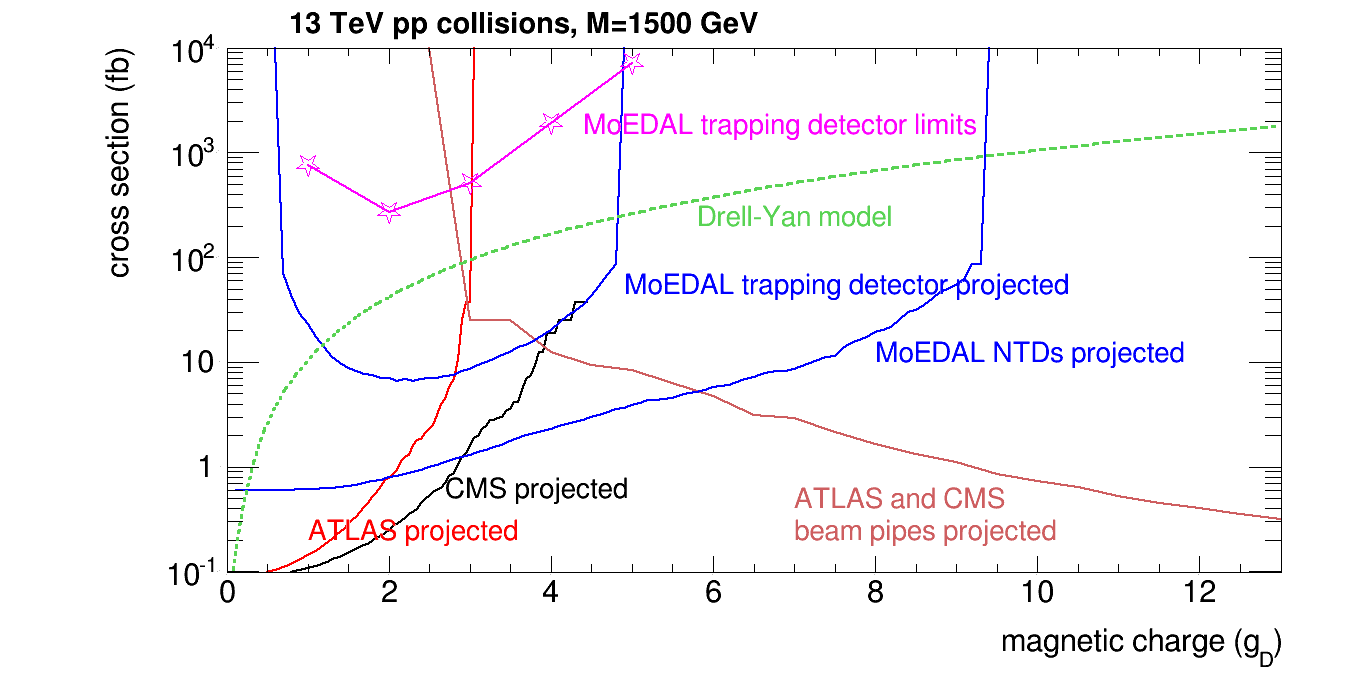
\includegraphics[width=0.8\textwidth]{plots/monopoles_xsec_13TeV_3events}
\caption{Comparison of the MoEDAL, ATLAS and CMS reach for magnetic monopoles. The curves assume 3 signal events and a total integrated luminosity of 50 fb$^{-1}$ for 13 TeV collisions. Source: private communication from P. Mermod, updated version of existing FIg. in~\cite{DeRoeck:2011aa}.}
\label{fig:magnetic_monopole_reach}
\end{figure}

\subsubsection{Quirks}

Quirks are particles charged under both the SM and a new confining gauge group \cite{Kang:2008ea}, referred to here as ``infracolor'' (IC). The defining property of quirks is that the tree-level quirk masses $m_Q$ are above the confinement scale $\Lambda_{IC}$ (this is like QCD but with no light-flavored quarks), so that there is never enough local energy density to pop new quirks out of the vacuum.  A pair of a quirk and an anti-quirk can live in a quantum mechanical bound state that can separate by macroscopic distances $\ell \sim \frac{m_Q}{\Lambda_{IC}^2}$, remaining connected by an infracolor flux tube. The infracolor flux tube exerts a tension on each quirk that causes its trajectory to differ from the expected helicoidal ones for SM particles. Although well-motivated by hidden-valley models \cite{Strassler:2006im}, we stress that quirks are not exclusive to hidden valleys, contrary to popular lore.

The collider phenomenology depends greatly on the size of $\ell$.  If $\ell$ is below the mm scale, the individual quirks are not distinguished from one another and the anomalous track can not be seen. However, the pair (which is overall neutral, and therefore does not bend in the tracker magnetic field) appears as a single highly ionizing straight track with missing energy aligned with it, the latter arising from miss-measuring the track momenta.
The D0 collaboration has searched for precisely this signature \cite{Abazov:2010yb}, requesting an additional jet for trigger purposes, finding lower bounds on quirk masses of 107, 119 and 133 GeV for SU(2), SU(3) and SU(5) gauge groups. However, no extensions of this search to higher mass have been performed at the LHC, and the existing HSCP searches require a fractional certainty on the tracks momenta that a straight track cannot provide.

Conversely, if $\ell$ is very large then the existence of the confining force has no effect on the quirk motions, and HSCP searches  apply directly to the quirk case, with quirks charged under QCD yielding $R$-hadrons and uncolored quirks leading to slepton-like signatures. We refer the reader to the HSCP section for more information.

For intermediate values of $\ell$, there are interesting phenomenological prospects at the LHC that have been recently studied theoretically~\cite{Farina:2017cts,Knapen:2017kly}, but for which there are no current public searches by the LHC collaborations. The first study~\cite{Farina:2017cts} has recasted mono-jet~\cite{CMS:2016pod,Aaboud:2016tnv} and HSCP searches, finding bounds up to 1.7 TeV for colored-quirk masses. In addition, it has also proposed using the CMS dataset taken with zero magnetic field. In this dataset, all SM particles are expected to follow a straight trajectory, but the quirks would still bend due to the string tension. The second study~\cite{Knapen:2017kly} has proposed a new algorithm to search for quirks, exploiting the fact that the quirk and anti-quirk pair should lie in the same plane with the highest sensitivity in the $\ell \sim 1-10$ mm range. This allows to avoid fitting the non-helicoidal trajectories, and has the potential to extend the sensitivity to quirks well beyond the current mono-jet and HSCP limits.

Because of the non-standard nature of the tracks, quirk phenomenology poses substantial challenges in their experimental reconstructions, and the lack of constraints on quirks have already attracted the attention of the ATLAS, CMS and LHCb experiments. It would be desirable to test how the phenomenological proposals in Refs.~\cite{Farina:2017cts,Knapen:2017kly} can perform in a realistic detector simulation of one of the LHC experiments.

\subsubsection{Strongly interacting massive particles (SIMPs)}

Strongly interacting massive particles (SIMPs) can be motivated by astrophysical observations of dark matter that do not fully agree with the WIMP paradigm (missing satellites, core-vs-cusp problem see e.g.~\cite{2010arXiv1009.4505B,2011MNRAS.415L..40B,Weinberg:2013aya,1742-6596-437-1-012001}). These particles are assumed to interact strongly with baryons. Consequently, the experimental signature is little to no signal in the tracker and the ECAL, and large energy deposits in the HCAL. Such a final state with trackless jets also arises in the context of emerging jets~\cite{Schwaller:2015gea}, and ATLAS has a trigger for trackless jets in association with a soft muon (where the muon is required to exit level 1 of the trigger)~\cite{ATLASLLPTriggers}. Additionally, the CalRatio trigger and associated search for displaced hadronic decays (addressed in Section~\ref{subsec:djets}) presents with a similar signature and could provide some coverage of this signature.  

An LHC phenomenological study of SIMPs was carried out in Ref.~\cite{Daci:2015hca}. We summarize the main points of the study here. In their setup, SIMPs interact with the SM via an attractive potential (either scalar or vector mediator) coupling SIMP pairs with $q\bar{q}$ pairs. The proposed analysis selects events with high \pT back-to-back jets within the tracker, exploiting the charged energy fraction within a jet to discriminate signal from background.  The astrophysical experimental constraints on this scenario are compared with the expected reach of this search and that of monojets in figure~\ref{fig:simps}. Currently there is an ongoing analysis in CMS pursuing this strategy.

\begin{figure}[htb]
\centering
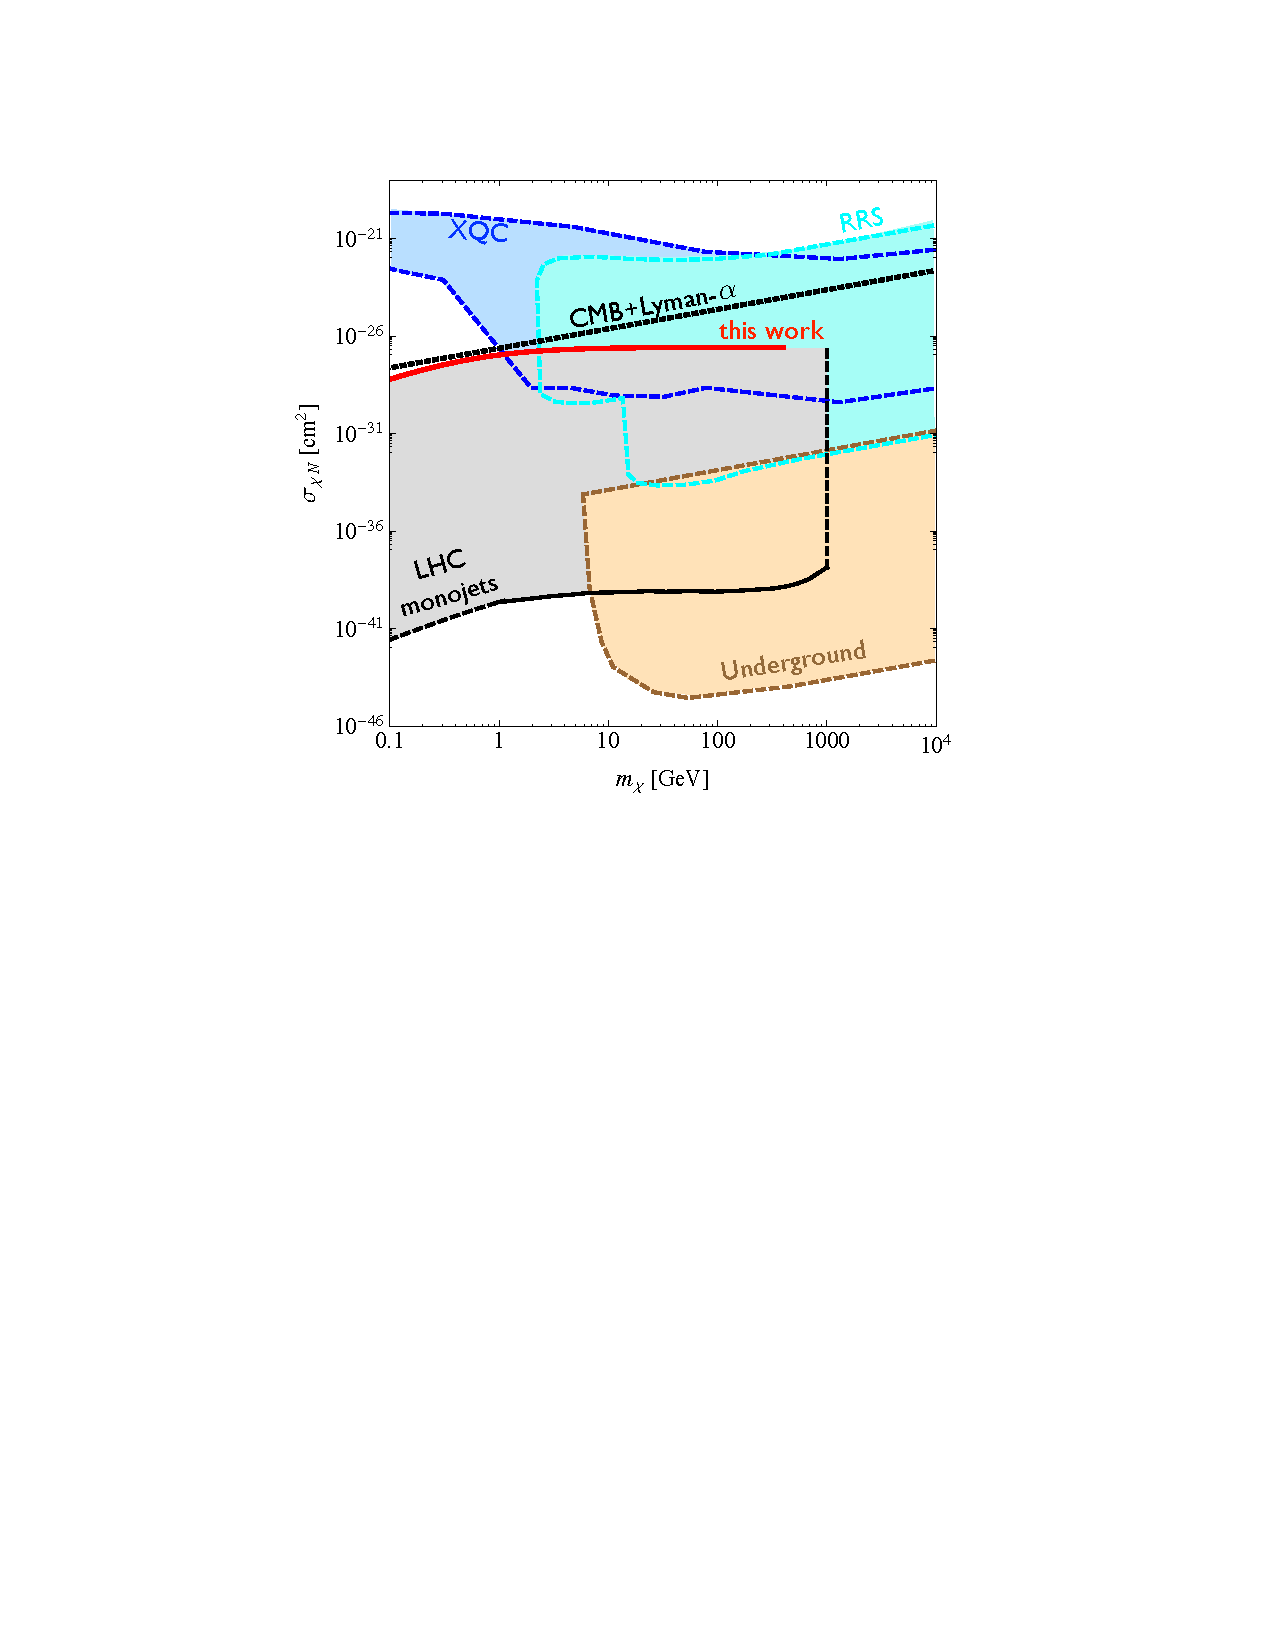
\includegraphics[width=0.5\textwidth]{plots/simps_constraints.pdf}
\caption{Astrophysical and collider constraints on a simple SIMP setup. Note that the relevance of the astrophysical constraints depends on the contribution of the SIMPs to the relic density. Taken from reference~\cite{Daci:2015hca}.}
  \label{fig:simps}.
\end{figure}


\section{Overview of Gaps}
\label{sec:covgaps}

\begin{enumerate}

	\item All-hadronic
	\begin{itemize}
	\item Use associated object triggers (especially motivated by Higgs like VBF and VH)
	\item Try to push to lower masses \& lifetimes
	\item Online reconstruction of hadronic displaced objects
	\item Exclusion limits for displaced hadronic taus. Opportunity for CMS displaced triggers?
	\end{itemize}

\item Leptonic	
	\begin{itemize}
	\item Intermediate region between low-mass (lepton-jets) and high-mass (resolved ATLAS/CMS searches)
	\item Continue to push to go to lower masses, $p_{\rm T}$ thresholds
	\item Tau leptons in LLP decay, in particular if they come from ID. Opportunity for CMS displaced triggers?
	\end{itemize}
	
	\item Semi-Leptonic	
	\begin{itemize}
	\item Low masses (like Majorana neutrino)
	\item Making sure to cover all flavor combinations (for example, one CMS search only covers $e^\pm\mu^\mp$), as well as same-sign vs.~opposite sign leptons
	\item Trigger on associated objects or use dilepton trigger if there are two LLPs?
%	\item 
	\end{itemize}
	

	
\item Photonic
	\begin{itemize}
	\item No coverage for LLPs decaying into $l \gamma$, $j \gamma$ or without $\metm$.
	\item Poor coverage (non-dedicated search) for single $\gamma$, only if two jets are present, needs recasting of CMS delayed photon study~\cite{CMS:2015sjc}.
	\item Prompt photons searches useless, as they veto "non-standard" photons.
	\item No coverage for softer photons.
	\end{itemize}
	
\item Other exotic long-lived signatures
	\begin{itemize}
	\item DTs: $c \tau \sim $ mm are very hard to probe. See suggestion in~\cite{Ito:2017dpm,Ito:2018asa}. Unclear if ATLAS IBL will be present in HL-LHC run. What is the lowest distance new layers (or double layers) can be inserted at? 
%	\item 
	\end{itemize}	

	

\end{enumerate}


%\bibliographystyle{JHEP}
%\bibliography{LLPs}
%
%
%\end{document}


\chapter{Reinterpretation and Recommendations for the Presentation of Search Results}

%\noindent {\bf Chapter editors:}~Giovanna Cottin, Nishita Desai, Zhen Liu, Andre Lessa, Sabine Kraml\\
%\text{ \; }\\
%\noindent {\bf Workshop working group conveners:}~Juliette Alimena, Will Buttinger, Jared Evans\\
%\text{ \; }\\
%\noindent {\bf Contributors:}~Eric Conte, Yanou Cui, Benjamin Fuks, Jan Heisig, Gavin Hesketh, Lukas Heinrich,  David Michael Morse, Michael Ramsey-Musolf, Ennio Salvioni, Michele Selvaggi, Brian Shuve, Yuhsin Tsai
%\text{ \; }\\

%%%%%%%%%%%%%%%%%%%%%%%%%%%%%%%%%%%%%%%%%%%%%%%%%%%%%%%%%%
\section{Introduction}
\label{sec:ch5-introduction}
%%%%%%%%%%%%%%%%%%%%%%%%%%%%%%%%%%%%%%%%%%%%%%%%%%%%%%%%%%

Models and scenarios with LLPs have seen an enormous rise in interest in recent years.
They include supersymmetric scenarios with almost mass-degenerate lightest states~\cite{Chen:1995yu,Feng:1999fu}, 
highly split spectra~\cite{ArkaniHamed:2004fb,Giudice:2004tc}, very weakly interacting 
lightest supersymmetric particles (LSPs) like gravitinos or 
axinos \cite{Pagels:1981ke,Covi:1999ty} or $R$-parity violation~\cite{Barbier:2004ez}, 
as well as equivalent scenarios in other SM extensions (e.g., extra-dimensional models) with new SM gauge-charged particles. 
More recent ideas include models with feebly interacting dark matter \cite{Hall:2009bx} (supersymmetric or not), asymmetric dark matter~\cite{Zurek:2013wia}, Hidden Valley~\cite{Strassler:2006im} and other dark sector models---see the classification of existing well-motivated theories with LLPs in Section~\ref{sec:simplifiedmodel} of this document.

All these models can feature a large variety of possible LLP signatures. In Hidden Valley models, for instance,   
new particles can either decay into invisible dark particles or back to the SM, thus possibly leading to a 
mix of long-lived and prompt signatures, with or without missing transverse energy (\MET). 
Furthermore, new theoretical frameworks are constantly emerging, often motivated by 
new approaches to the hierarchy problem or dark matter. 
It is therefore of great interest to our community to be able to 
re-interpret the LLP experimental results 
for new models, which may be brought up in the future.\footnote{In this context we refer the reader also to 
the activities of the ``Forum on the Interpretation of the LHC Results for BSM studies''~\cite{reinterpretationForum}, which brings together more than 100 theorists and experimentalists around this topic.}

The re-interpretation can generically be done in two ways, either applying
appropriate simplified-model results, or reproducing the experimental analysis in a Monte Carlo simulation. Clearly,  the former is easier and faster, 
while the latter is more general but more difficult and much more time consuming~\footnote{When no new backgrounds 
need to be considered and the hypothesised signal does not affect control regions, one can simply determine the 
event counts in the signal regions and compare them to the $95\%$ C.L observed limits, or take the numbers of observed events and expected backgrounds to compute a likelihood.}. 

In the context of searches for prompt signatures with \MET, the use of simplified models has been shown to be a fruitful approach for both the experimental and theoretical communities~\cite{hep-ph/0703088, 0810.3921, 1105.2838, Okawa:2011xg,1301.2175,Boveia:2016mrp}. 
Dedicated tools~\cite{Kraml:2013mwa,Ambrogi:2017neo,Papucci:2014rja} are publicly 
available and allow the user to re-interpret SUSY simplified-model results within the context of a full model.
The coverage of a full model can, however, be severely limited by the kind of simplified-model results available, 
as discussed recently in \cite{Ambrogi:2017lov} for the case of the phenomenological MSSM.
Indeed, for some models the large number of relevant simplified-model topologies and their complexity
can make the simplified-model approach inexpedient. 
%Limitations also arise when the signal acceptance depends on the details of the model 
%(e.g., the spin- and coupling structure, the assumed production modes, etc.).  
%In both these cases, insufficient coverage by available simplified models and model dependence of the signal acceptance, 
In this case, a more complete and robust recasting procedure is necessary. 

Again, for prompt signatures, a general recasting approach is available through several public 
tools, notably \textsc{CheckMATE}~\cite{Drees:2013wra,Dercks:2016npn}, \textsc{MadAnalysis5}~\cite{Conte:2014zja,Dumont:2014tja}, 
\textsc{Rivet}~{\bf\cite{Buckley:2010ar}} (v2.5 onwards) and Gambit's \textsc{ColliderBit}~\cite{Balazs:2017moi}.
These tools allow to reproduce experimental analyses by means of Monte Carlo event simulation coupled to 
an approximate emulation of detector effects.\footnote{For completeness it should be noted that, while all these tools include a more or less 
extensive set of SUSY searches, many of the searches for other, ``exotic'' types of new physics cannot yet be reproduced outside the experimental collaborations. This concerns in particular searches relying on BDT or MVA techniques.} 
For the latter, \textsc{CheckMATE} and \textsc{MadAnalysis5} rely on \textsc{Delphes3}~\cite{deFavereau:2013fsa}, 
in some cases supplemented with appropriate tuning, 
while \textsc{Rivet} and \textsc{ColliderBit} employ object smearing and analysis-specific reconstruction efficiencies. 
The ATLAS and CMS collaborations are helping these recasting efforts by providing more and more 
detailed information about their analyses and results. As an example, covariance matrices for the background correlations in the framework of simplified likelihoods were provided for the analysis of Ref~\cite{CMS-NOTE-2017-001}.

The situation is --so far-- quite different for LLP searches. 
First, the presentation of results in terms of simplified models 
is still limited to few topologies and does not always include all the
parameters required for a general purpose re-interpretation. 
Notice here that, compared to simplified models for prompt searches, simplified models 
for LLP searches always have at least one additional degree of freedom --the lifetime of the LLP. 
Second, general purpose recasting tools are not yet available.
Recasting LLP searches outside the experimental collaborations is  a
difficult task, since they are very sensitive to the detector response, which in most cases 
cannot be easily emulated (or not even described, as for the backgrounds presented in 
Chapter~\ref{sec:backgrounds}) by a fast detector simulation.
As a result, none of the available (public) tools can currently recast
LLP searches, thus rendering the applicability of the experimental
results extremely limited. 


In order to allow for a more extensive re-interpretation or recasting of 
the experimental analyses, detailed information concerning the detector
performance and object reconstruction is needed.
These can in principle be provided in the format of efficiencies\footnote{We
employ the term ``efficiency'' in a broad sense. It can refer to reconstruction
efficiencies, selection efficiencies, overall signal efficiencies, etc. which will be further specified below.}
for selection and reconstruction of relevant objects, as demonstrated
already by some pioneering experimental publications~\cite{Khachatryan:2015lla,Aaboud:2017iio}.
One difficulty in this respect is that the information needed for recasting LLP searches is clearly
analysis-dependent, which means an additional workload for the analysis groups to provide this information 
case by case.  

\begin{figure}[t]
\begin{center}
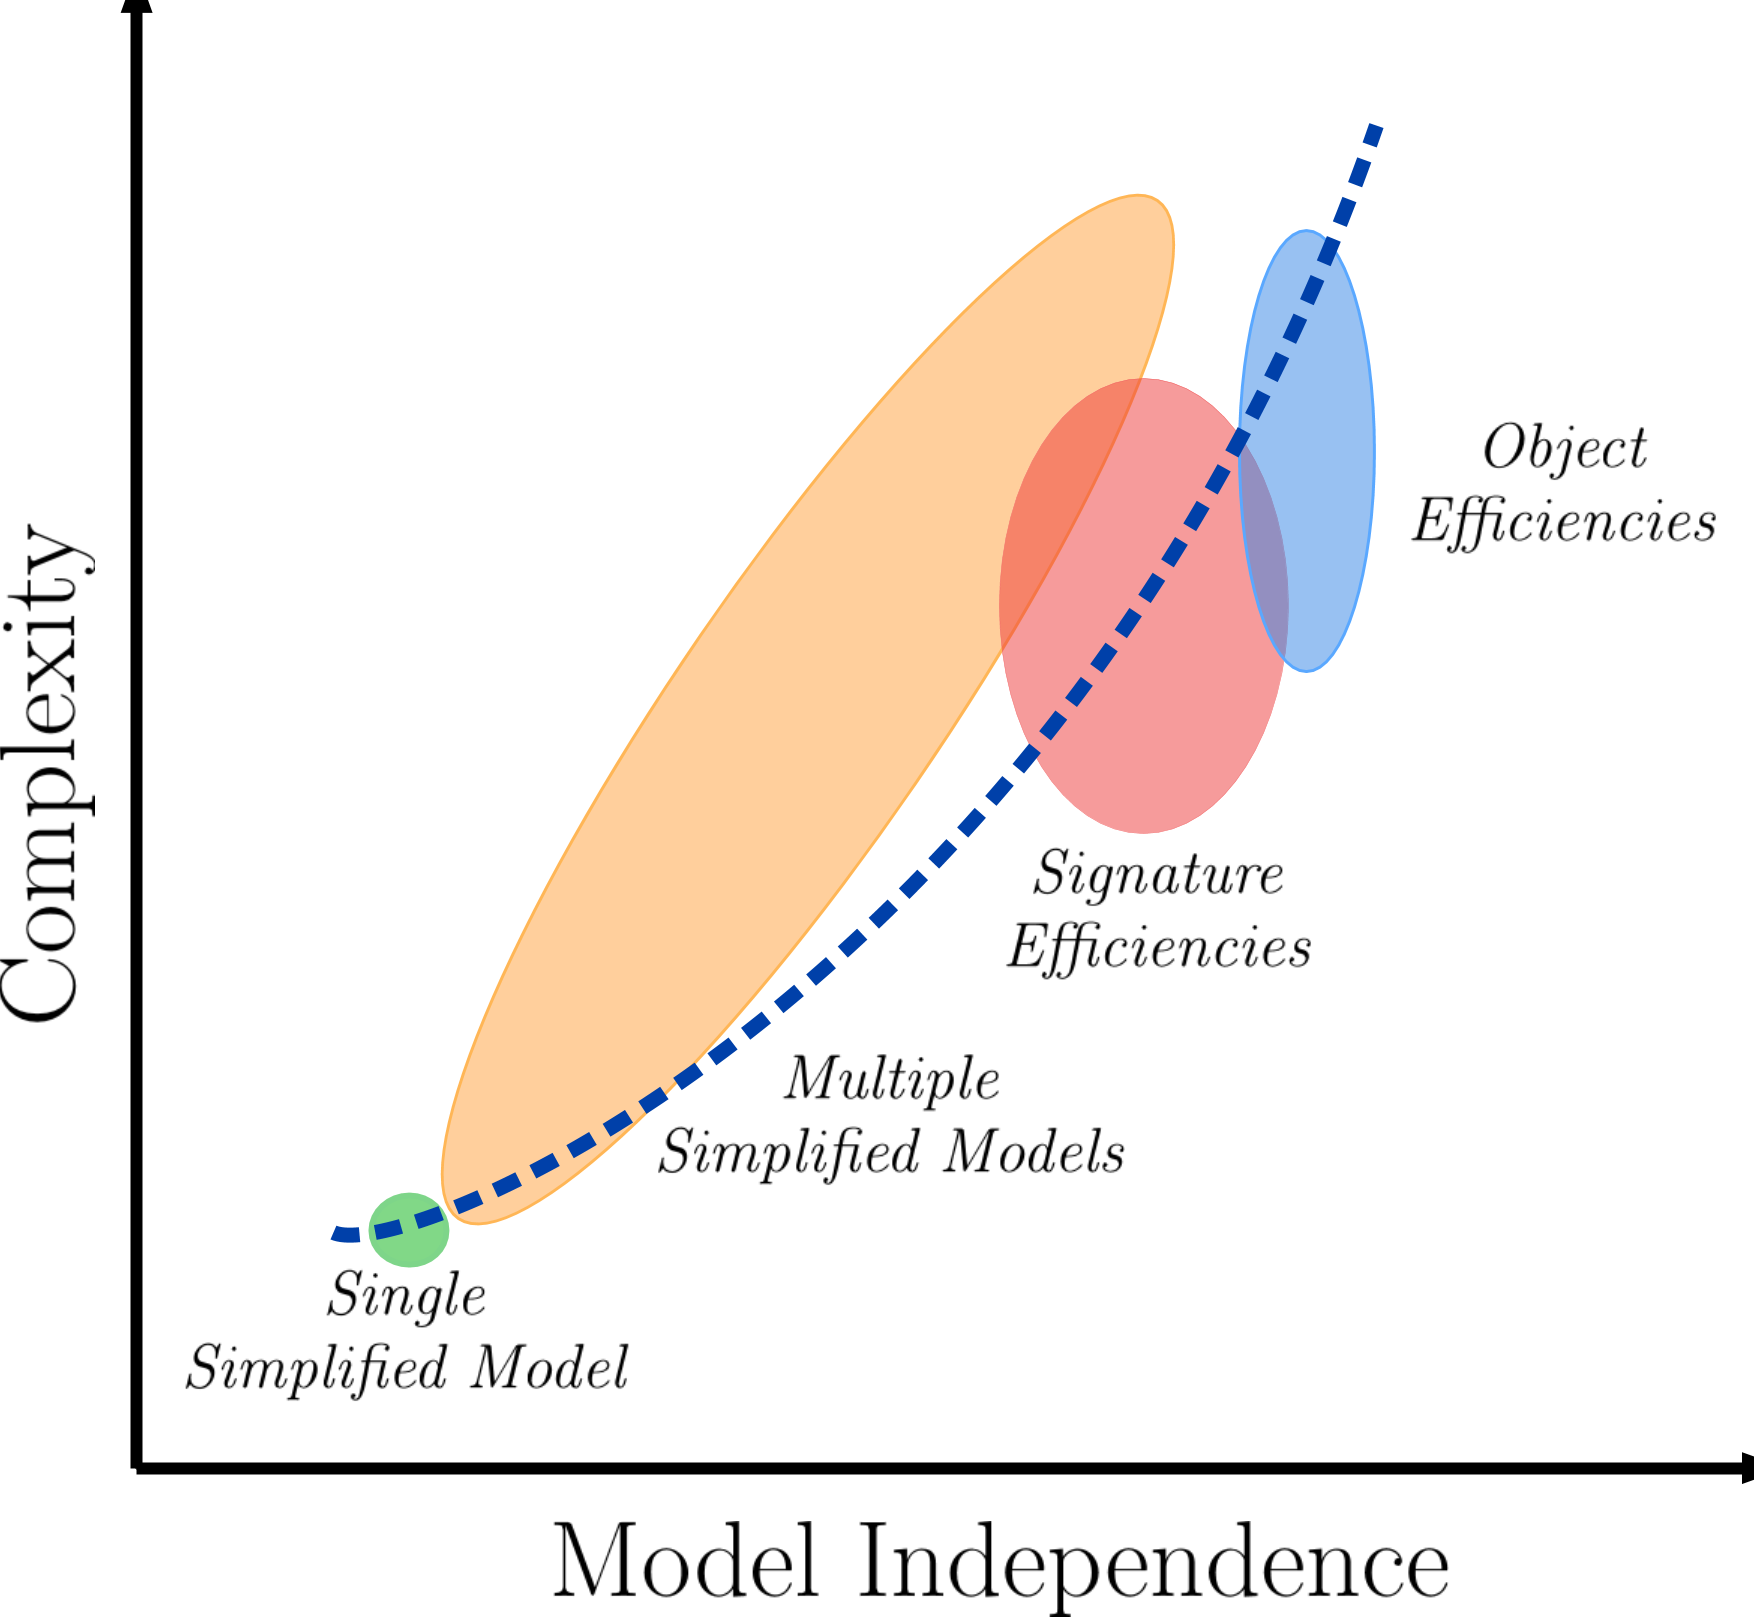
\includegraphics[width=0.7\textwidth,angle=0]{ch5-figures/LLP_interpretationsB.png}
\end{center}
\caption{A qualitative overview of the possibilities
for results presentation discussed in this chapter.
The axes represent the complexity of information required by each
format and the corresponding level of model independence.}
\label{fig:ch5-complexity-vs-modelindependence}
\end{figure}

The objective of this chapter is to discuss the presentation of the LLP search results  
with the aim that they can be re-used for interpretations beyond the models considered in the 
experimental publications.  
To this end, we first discuss in Section~\ref{sec:ch5-options} the various options 
for presenting the LLP results, see Fig.~\ref{fig:ch5-complexity-vs-modelindependence}, and compare their advantages and
shortcomings. 
In Section~\ref{sec:ch5-smsReinterpretations} we discuss in more details how the simplified models defined in Section~\ref{sec:simplifiedmodel} can be used to re-interpret LLP searches. 
In Section~\ref{sec:ch5-recastExamples}, we present several attempts of recasting LLP searches, 
according to the LLP signature: heavy stable charged particles and displaced objects; for each case, 
the lessons learned are elaborated. 
Section~\ref{sec:ch5-recastingDelphes} presents a first attempt to
extend the public detector simulator \textsc{Delphes} %and the recasting tool MadAnalysis5 
to deal with LLP searches, while 
Section~\ref{sec:ch5-recastingInsideExp} deals with reinterpretations performed within the experiments themselves, 
including the RECAST framework.  
In Section~\ref{sec:ch5-recastingPrompt}, we discuss complementary constraints on LLPs from re-interpreting prompt searches. 
We conclude in Section~\ref{sec:ch5-rec_summary} with our %suggestions and 
recommendations for the presentation of LLP results. 


%%%%%%%%%%%%%%%%%%%%%%%%%%%%%%%%%%%%%%%%%%%%%%%%%%%%%%%%%%
\section{Options for Presenting Experimental Results} 
\label{sec:ch5-options}
%%%%%%%%%%%%%%%%%%%%%%%%%%%%%%%%%%%%%%%%%%%%%%%%%%%%%%%%%%

A qualitative view of the various possibilities for presentation
of search results is given in
Fig.~\ref{fig:ch5-complexity-vs-modelindependence}.
We broadly classify these possibilities according to the type of
information provided or type of efficiency.
Each type refers to distinct signal objects, as illustrated in
Fig.~\ref{fig:ch5_presentation_options}.
As we can see, each possibility relies on distinct assumptions about
the signal, resulting in different levels of model-dependence.
Below we provide a brief discussion of the advantages and limitations of the
various possibilities of presentation of LLP search results.
We will gradually progress from the simplest case towards more complexity but
also better re-usability.


% Let us start with the presentation of results in the context of simplified
% models (for a list of proposed simplified models see {\color{blue}{Chapter~\ref{whitepaper:simplified-models}}}).
{\bf Simplified Models}: %the most commonly used format for the presentation of
%results is simplified model upper limits or efficiencies.
In most cases the simplified-model topology corresponds to single or pair
production of the LLPs, though in principle simplified models for production
through cascade decay of heavier states can also be envisaged. 
In any case, the simplified model incorporates important assumptions 
on the LLP production, decay mode and quantum numbers. 
%The search results are typically presented as  95\% CL limit curves, cross section upper limits and/or signal efficiencies.
Simplified-model results can be presented at different levels of sophistication and re-usability:
\begin{itemize}
\item exclusion curves in, e.g., a mass-vs-mass or mass-vs-lifetime plane, are highly model dependent and can 
rarely be used for re-interpretation;
\item cross-section upper limits\footnote{For the sake of re-usability, cross section upper limits in absolute terms are much preferred over limits on the signal strength.} 
can be applied to a larger variety of models
in which the same LLP production and decay mode occurs 
through a rescaling of the cross section times branching 
ratio factor; 
\item simplified-model efficiencies allow to go one step further: they make
it possible to combine different topology contributions to the same signal
region and compute an approximate likelihood using the number of expected and
observed events.
\end{itemize} 

% \noindent
The main advantages of simplified models are a parametrization in terms of few
physical parameters and a unified language and format applicable to a wide range of searches.
Also, when re-using simplified-model results one avoids detector simulation uncertainties. 
The disadvantages are that the simplified-model result  
cannot be applied to other LLP production or decay modes, resulting
in too conservative limits if the LLP signal is composed from
multiple topologies. This can be considerably relevant if 
the LLP is a color singlet, but there are several heavier color-charged states
which can be produced and decay to the LLP.
In principle this can be overcome if efficiencies are provided for a
sufficiently large number of simplified models (including cascade decays), as a
function of the simplified-model parameters, which should include the LLP lifetime.
These efficiencies can then be combined in order to compute the corresponding
constraints to complex models, where multiple topologies are present.
\footnote{These points are illustrated by the re-interpretation of the CMS search
for heavy stable charged particles~\cite{Khachatryan:2015lla}
discussed in Section~\ref{sec:ch5-smsReinterpretations}: 
for the specific model considered in \cite{Heisig:2015yla},
constraints obtained using only a single simplified model (direct production of
$\tilde{\tau}$s in this case) can underestimate the bounds on the LLP mass by almost a factor of two.}
We stress, however, that in order for this combination to be possible, signal efficiencies and 
not cross-section upper limits must be provided.
The major drawback of this approach is that in order for the results to be
applicable to a broad class of models, the number of required simplified models
and their complexity can easily become very large.
For achieving a high level of model independence, it is therefore desirable 
that the experimental analysis can be recast with Monte Carlo event simulation. 
Two ways of presenting results are useful to this end: {\it signature
efficiencies} and {\it object efficiencies}. 



\begin{figure}[t]
\begin{center}
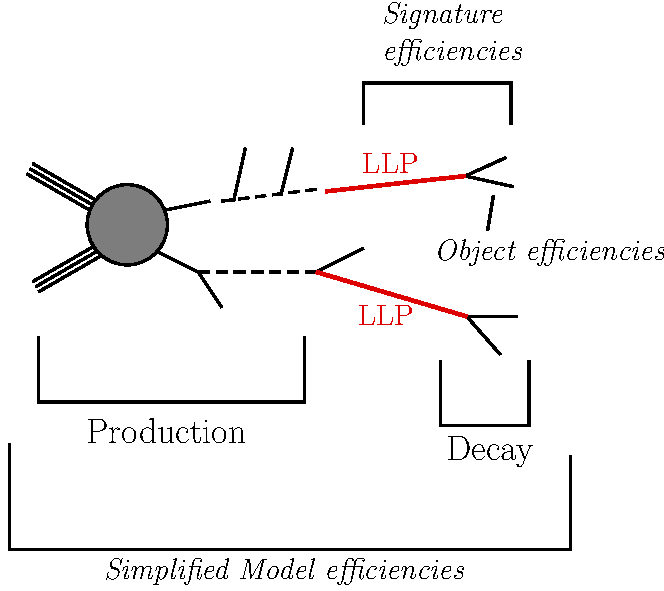
\includegraphics[width=0.6\textwidth,angle=0]{ch5-figures/LLPdiagramScheme.pdf}
\end{center}
\caption{Possibilities for the presentation of results: 
simplified-model efficiencies assuming a specific topology of LLP production and decay, 
signature efficiencies assuming only a specific LLP decay, and object efficiencies which are 
independent of the specific decay mode.
}
\label{fig:ch5_presentation_options}
\end{figure}


  
{\bf Signature efficiencies} are efficiencies for the reconstruction of the
main LLP signature (single charged track, displaced vertex, disappearing
track, \ldots) as a function of the LLP kinematical parameters and
the lifetime. 
Signal efficiencies require the assumption of a specific LLP decay, but 
are highly model independent, since they make no assumption on the LLP
production mode.
In addition, they are fully model-independent for stable particles
(within the detector dimensions), since in this case no assumptions about
the LLP decay mode are required.
In many cases, however, the reconstruction efficiencies depend on multiple
variables, such as the LLP $p_T$, its transverse decay position, impact
parameter, etc. 
As illustrated in section~\ref{sec:ch5-displacedVertices}, these efficiencies
could be very useful for recasting LLP searches, but often they 
are not provided by the experimental collaborations. Many recasting efforts consist in 
extracting these efficiencies from the provided information, but can result in large uncertainties. 

{\bf Object efficiencies} are efficiencies for the reconstruction of
the physics objects relevant for building the LLP signature. 
They can clearly be applied to a wide range of LLP
decay and production modes, since no specific assumptions about these are
required. 
For instance, a displaced lepton reconstruction efficiency can be provided
as a function of the lepton $p_T$ and its production position.
As discussed in Section~\ref{sec:ch5-displacedLeptons}, these efficiencies
can be used to recast LLP searches to an acceptable accurary ($\sim 20\%$).
Furthermore, as illustrated in Section~\ref{sec:ch5-displacedVertices},
knowledge of object efficiencies are essential for a general purpose
recasting of the search.
Within this approach the model dependence is minimal and can be
restricted to a few general assumptions about the nature of the LLP.
Also, object efficiencies could be included in fast
detector simulators, thus providing a way of recasting LLP searches
on the same footing as prompt searches. 
The main difficulty with providing such object efficiencies is
the potentially large number of parameters required for their parametrization.


%%%%%%%%%%%%%%%%%%%%%%%%%%%%%%%%%%%%%%%%%%%%%%%%%%%%%%%%%%
\section{Reinterpretation using Simplified Models}
\label{sec:ch5-smsReinterpretations}
%%%%%%%%%%%%%%%%%%%%%%%%%%%%%%%%%%%%%%%%%%%%%%%%%%%%%%%%%%

One of the possibilities for extending the experimental results from LLP
searches to a large variety of scenarios is through the use of simplified-model topologies.
Simplified models (or simplified-model spectra, SMS) have been widely used for the interpretation of
prompt and LLP searches. As discussed in Chapter~\ref{sec:simplifiedmodel}, a large
number of SMS topologies are possible for the distinct LLP signatures, which
can be grouped by the LLP production mode, decay and lifetime.
These SMS topologies aim to capture the main physical properties of the LLP
signal and can then be used to constraint other scenarios containing similar
topologies.
The use of simplified-model results to constrain full models has been
shown to be possible~\cite{Kraml:2013mwa,Papucci:2014rja,Belanger:2015cra,Barducci:2015zna,Arina:2015uea,Ambrogi:2017lov}, 
even though it has its shortcomings~\cite{Ambrogi:2017lov}.
Also within the context of LLP searches, the use of
simplified model results for re-interpretation can be a good alternative, \emph{e.g.,}
when a recasting based on a MC simulation is difficult or
is too computationally  expensive.
In this section, we briefly review how 
SMS results can be used to re-interpret searches for full
models as well as the particular challenges presented by LLP searches.
A concrete example of re-interpretation using simplified models is given in
Sec.~\ref{sec:ch5-smsHSCP}, based on the results of Ref.~\cite{Heisig:2015yla}.

\subsection{From Simplified to Full Models}

The interpretation of experimental results using
simplified models typically correspond to upper limits on the production
cross section or signal efficiencies for a specific SMS topology (production and
decay channel). These results are provided as a function of the simplified model
parameters, which have been largely taken to be the masses of the BSM
particles appearing in the topology. For LLP topologies, however, 
a new parameter must be considered: the LLP lifetime (see Chapter~\ref{sec:simplifiedmodel}).
With the exception of searches for stable particles, the lifetime is one of the
main parameters affecting the topology efficiency and upper limit.

Once signal efficiencies\footnote{For simplicity we will refer to the signal
acceptance times efficiency as ``signal efficiency''. This efficiency
is a function of the simplified model parameters, including the LLP lifetime.}
($\epsilon$) are provided for one or more SMS topologies, these can be used, under some
approximations, to quickly compute the number of expected signal events ($S$)
for a full model:
\begin{equation}
S = \mathcal{L} \times \left( \sum_{\text{SMS}} \sigma_{\sms}
\times BR_{\sms} \times \epsilon_{\sms} \right) \, ,
\label{eq:decomp}
\end{equation}
where $\mathcal{L}$ is the luminosity for the respective search and the sum runs
over simplified model topologies. Since the production cross-section
($\sigma_{\sms}$) and branching ratios ($BR_{\sms}$) for each topology
can be quickly computed for any full model, the simplified model
signal efficiencies ($\epsilon_{\sms}$) can be directly used to
obtain the signal yield. This procedure does not rely
on any Monte Carlo simulation or recasting of LLP searches and
can be easily applied to a wide variety of models, provided $\epsilon_{\sms}$
is known.
The main limitation of this approach comes from the limited (although
growing) number of SMS results available. Since $\epsilon_{\sms}$ is typically
known only for very few simplified models, the sum in Eq.~\eqref{eq:decomp} is
limited to the number of available topologies, resulting in an under-estimation of $S$.

For prompt SUSY searches, a systematic approach for
re-interpreting simplified model results based on the procedure
outlined above has been developed in Refs.~\cite{Kraml:2013mwa,Papucci:2014rja}.
Furthermore, using the large number of available SUSY SMS results, 
public tools are available for constraining full models using these
results~\cite{Ambrogi:2017neo,Papucci:2014rja}.
The same procedure can also be applied to LLP SMS results, as 
shown in Ref.~\cite{Heisig:2015yla} for the case of 
heavy stable charged particles (HSCPs) and implemented recently in \textsc{SModelS}~\cite{Heisig:2018kfq}.  %for HSCPs and R-hadrons. 
In the next section we review some of the results found in
Ref.~\cite{Heisig:2015yla}. Although these have been obtained within the
context of HSCPs, the main results can be generalized to other LLP
signatures, and demonstrate some of the advantages and shortcomings of
re-interpretations using LLP simplified models. 


\subsection{Reinterpretation using HSCP Simplified Models}
\label{sec:ch5-smsHSCP}

The CMS search for HSCPs in Ref.~\cite{Khachatryan:2015lla}
provided signal efficiencies for the following simplified model topology:
$ pp \to \tilde{\tau} \tilde{\tau}$ as a function of the
stau mass. In the language of the simplified models of Sec.~\ref{sec:EMcharge},
this is the direct pair production mode of a charged LLP.
 The stau is assumed to be stable (at detector scales), thus
producing a highly ionizing track, which can be used to search
for this scenario (see Sec.~\ref{subsec:funnytracks}). 
Since the stau lifetime ($\tau$) is assumed to be $\gg
10$~ns, the signal efficiencies do not depend on $\tau$,
thus simplifying the SMS parameter space, which reduces to the stau
mass.\footnote{We point out that it is still possible to apply these simplified
model results to models with smaller LLP lifetimes if we include the suppression
factor from the LLP decay length distribution, as
discussed in Sec.~\ref{sec:ch5-validate}.
}
The relevant selection efficiencies required for a general purpose
MC recasting of the HSCP search have also been provided by
the CMS analysis (see Sec.~\ref{sec:ch5-HSCPs} for details).


The efficiencies for the stau simplified model
can be used to constrain a full BSM scenario which contains
HSCPs. In Ref.~\cite{Heisig:2015yla}, the region of the CMSSM parameter
space with $m_{\tilde \tau} - m_{\tilde \chi_1^0} < m_{\tau}$ has been
considered, since it provides a possible solution to the Lithium
problem~\cite{Spite:1982dd, Cyburt:2008kw}. Due to the small
mass difference, the stau is long-lived and decays outside the detector,
thus generating a HSCP signal.
In Fig.~\ref{fig:cmssmA}, we show the constraint on the CMSSM parameter
space obtained using only the simplified model provided by CMS (direct stau
production).
Since the simplified model only contains one parameter, it
translates to a limit on the stau mass ($m_{\tilde \tau} < 260$~GeV),
as shown by the blue region in Fig.~\ref{fig:cmssmA}.
In this CMSSM scenario, however, direct production of staus only contribute to a
small fraction of the total HSCP signal, since staus are typically produced from
cascade decays of heavier SUSY states, such as charginos, squarks and gluinos 
(these are the heavy-parent modes of Sec.~\ref{sec:EMcharge}).
Furthermore, there are several possible topologies which contains a stau and the
LSP ($\tilde \chi_1^0$) in the final state, thus resulting in a
mixed missing energy-HSCP signature.
Therefore using only the CMS constraints for the direct stau production
simplified model largely underestimate the sensitivity of the CMS
search. 


\begin{figure}[t]
\centering
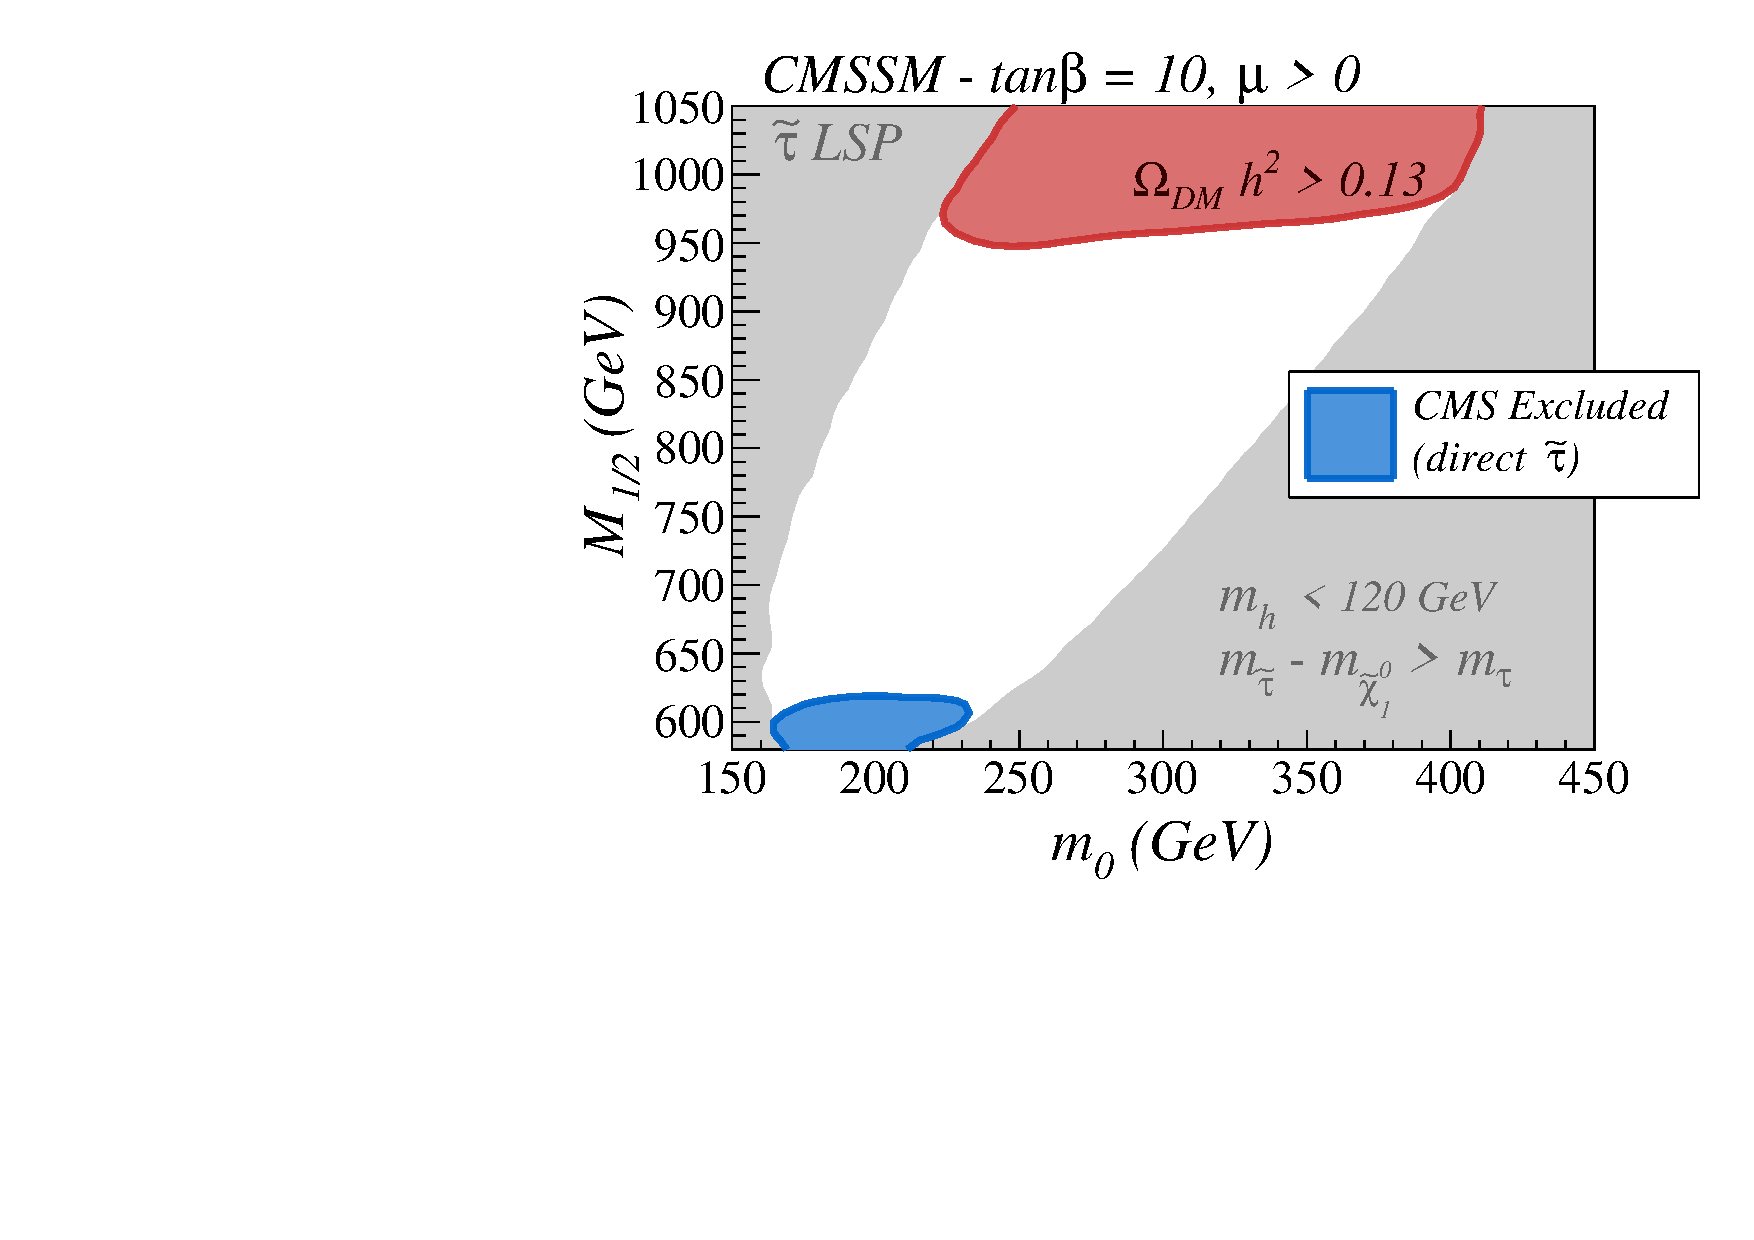
\includegraphics[width=0.8\textwidth]{ch5-figures/sms_exclusion_direct.pdf}
\caption{Region of the CMSSM parameter space with long-lived NLSP staus.
The light gray regions are excluded by the requirements $m_{\tilde \tau} \gtrsim
m_{\tilde \chi_1^0}$ and $ 120 \mbox{ GeV} \leq m_h \leq 130 \mbox{ GeV}$.
The top red region is excluded by the upper limit on the neutralino relic
density, while the lower blue region is excluded by the CMS constraints
on direct production of long-lived staus. For more details see Ref.~\cite{Heisig:2015yla}.
}
\label{fig:cmssmA}
\end{figure}


In order to improve the constraints shown in Fig.~\ref{fig:cmssmA}, one must
have efficiencies for several SMS topologies. Fortunately, a MC
recasting of the 8~TeV CMS search is possible (see Sec.~\ref{sec:ch5-HSCPs} for details)
and can be used to compute simplified model efficiencies.
In Ref.~\cite{Heisig:2015yla}, seven additional simplified models containing
cascade decays were considered and their efficiencies computed as a function of
the masses appearing in the topology. A summary of the topologies considered
are shown in Table~\ref{tab:defModels}. It is important to point out that
it is not necessary to specify the Standard Model final states appearing in the
simplified models, since the HSCP search is inclusive and the efficiencies
do not depend on the additional event activity.
Using this extended database of simplified model efficiencies
and Eq.~\eqref{eq:decomp}, we can compute a more inclusive signal yield for each
point of the CMSSM parameter space and improve the constraints on the model.
The results are shown in Fig.~\ref{fig:cmssmB}, where
we see a drastic improvement in the region excluded by
the constraints on HSCPs, as expected.
For this specific scenario (with
$\tan\beta = 10$), all the parameter space is excluded either by the CMS or dark matter
constraints~\cite{Heisig:2015yla}.


\begin{table}
\begin{center}
\begin{tabular}{lcc}
\toprule
SMS topology & Notation in Chapter~\ref{sec:simplifiedmodel}
% & parameters 
%& SUSY\;process
\\
\midrule
$pp \to X\;X$ & DPP
% & $m_{\text{HSCP}}$ 
% & $pp\to \charg \charg$ 
\\
$pp \to Y_1\;Y_1, Y_1\;\to SM\;X$ & HP
% & $m_{\text{HSCP}},m_{\text{prod}}$ 
%& $pp\to \sq\sq\to \charg \charg$ 
\\
$pp \to Y_1\;Y_1, Y_1\;\to SM\; Y_2, Y_2\;\to SM\;X$ & -
% & $m_{\text{HSCP}},m_{\text{int}},m_{\text{prod}}$ 
%& $pp\to \sq\sq\to \neu \neu\to\stau_1\stau_1$ 
\\
$pp \to Y_1\;Y_2, Y_1\;\to SM\;Y_2, Y_2\;\to SM\; X$ & -
% & $m_{\text{HSCP}},m_{\text{int}},m_{\text{prod}}$ 
%& $pp\to \neu\s\chi^\pm_2\to \stau_1 (\charg\to\stau_1)$ 
\\
$pp \to Y\;Y, Y\;\to SM\;SM\;X$ & HP
% & $m_{\text{HSCP}},m_{\text{prod}}$ 
%& $pp\to \sq\sq\to \stau_1\stau_1$ 
\\
$pp \to inv\; X$ & CC
% & $m_{\text{HSCP}} = m_{\text{inv}}$ 
%& $pp\to  \charg \neu$ 
\\
$pp \to Y_1\;Y_2, Y_1\;\to SM\;inv, Y_2\;\to SM\;X$ & -
% & $m_{\text{HSCP}},m_{\text{prod}}$
%&  $pp\to \sq\sq\to \charg \neu$ 
\\
$pp \to Y_1\;Y_2, Y_1\;\to SM\;inv, Y_2\;\to Y_3\;SM, Y_3\;\to SM\;X$ & -
% & $m_{\text{HSCP}},m_{\text{int}},m_{\text{prod}}$
%&  $pp\to \sq\sq\to \neu (\neu\to\stau_1)$ 
\\
\bottomrule
\end{tabular}
\end{center}
\caption{Definitions of the HSCP simplified models considered in this Section.
$X$ represents the HSCP, $Y_i$ represent intermediate BSM particles,
$SM$ represents any Standard Model particle and $inv$ represents an invisible
final state, such as the neutralino. The correspondance with the simplified models language 
of Chapter~\ref{sec:simplifiedmodel} (section~\ref{SM:secProduction_modes}) is also given.}
\label{tab:defModels}
\end{table}



\begin{figure}[!h]
\centering
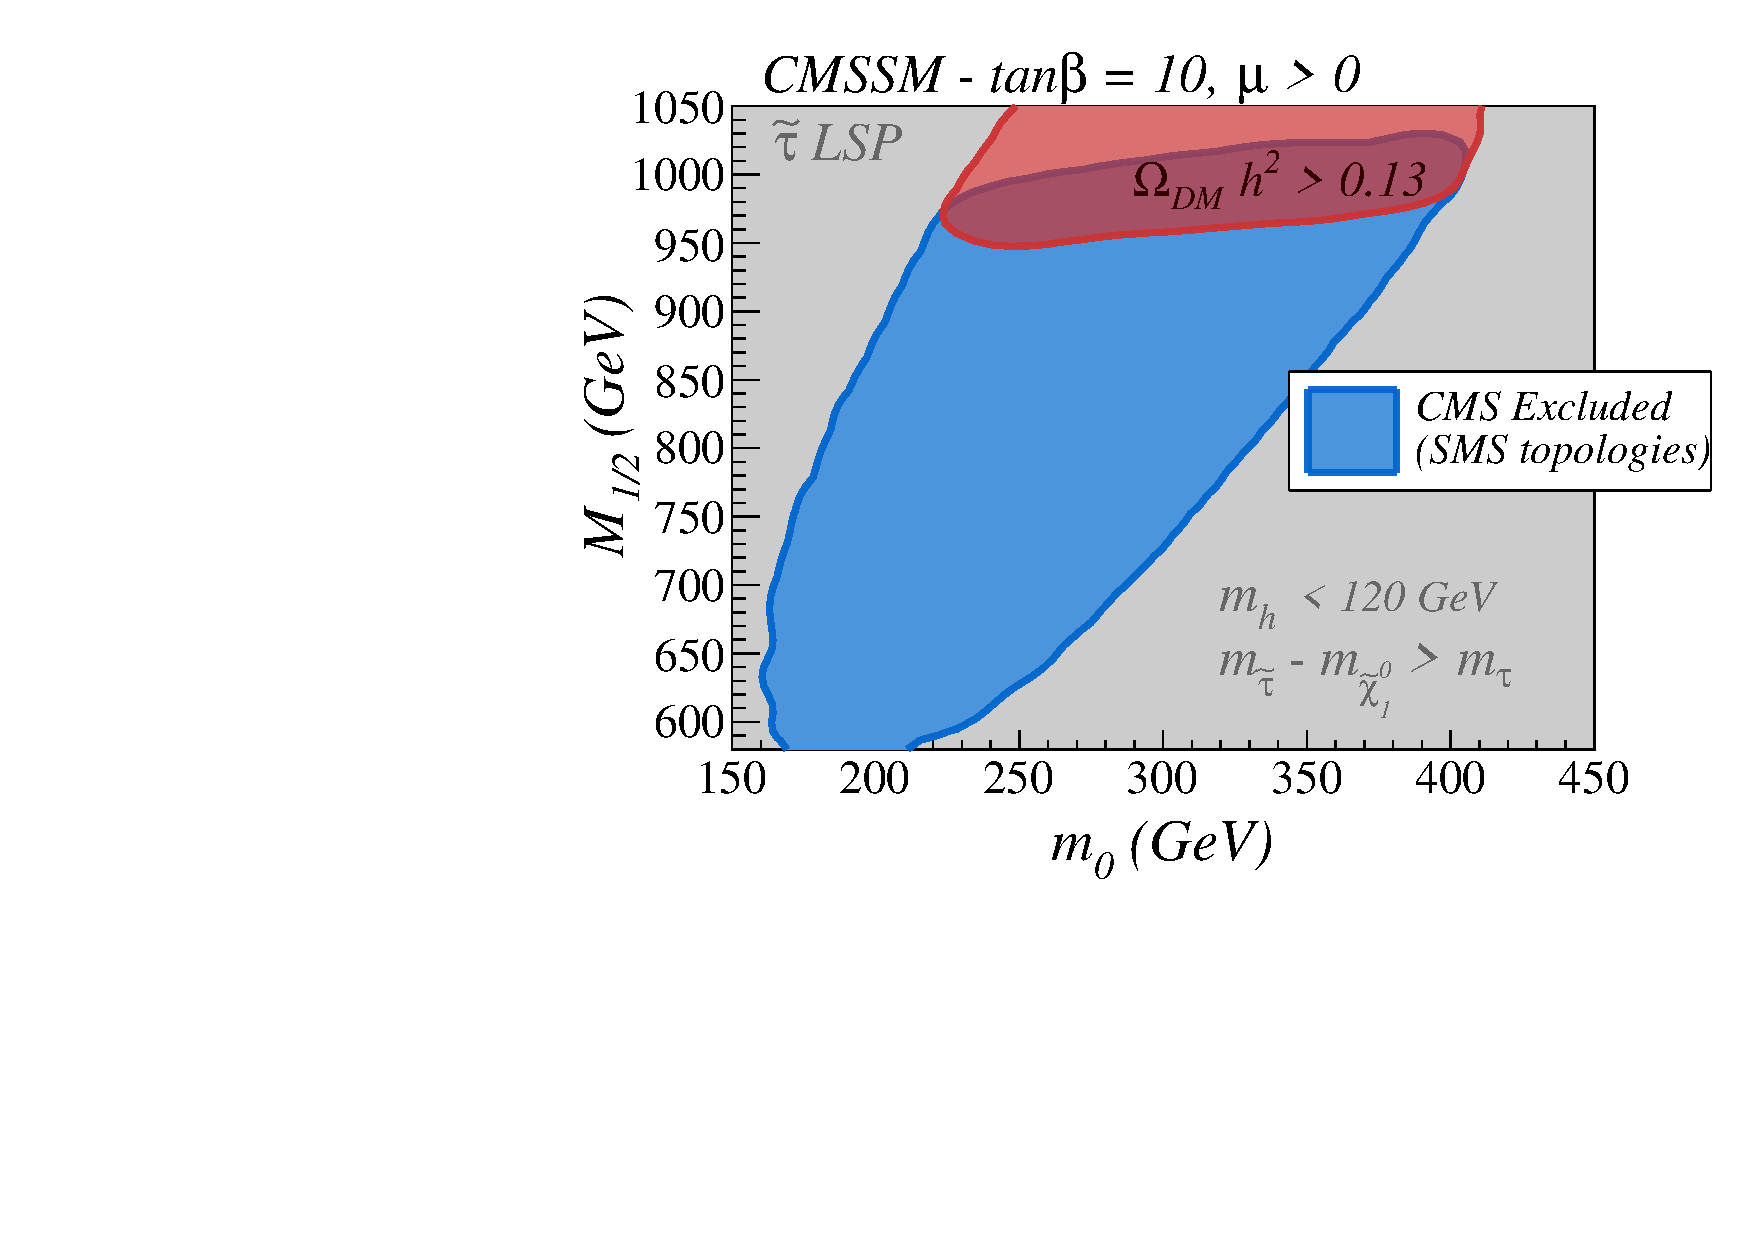
\includegraphics[width=0.8\textwidth]{ch5-figures/sms_exclusion_all.pdf}
\caption{Same as Fig.~\ref{fig:cmssmB}, but using all the simplified
models listed in Table~\ref{tab:defModels}.
}
\label{fig:cmssmB}
\end{figure}


Fig.~\ref{fig:cmssmB} illustrates the feasibility of using simplified
model efficiencies to constrain full models.
This approach has the advantage of being computationally inexpensive
(once the efficiencies are known) and can be used to quickly test
a large number of model points. However the approach relies on a few
approximations and is never fully inclusive, since the number of  SMS topologies
with published efficiencies is always limited.
Hence, it is important to verify
how close the simplified model re-interpretation comes to the full recasting
using a Monte Carlo simulation.
In Ref.~\cite{Heisig:2015yla} it was shown that, within
the CMSSM scenario discussed above and using eight simplified model
topologies, the SMS results reproduce the full simulation within
20\% or better.
Since this error is of the order of the uncertainties in recasting,
the use of simplified models becomes a viable alternative to full recasting.
The SMS re-interpretation is  even more relevant for the cases
where a straightforward MC recasting is not possible.


\vskip 0.1in
\noindent {\bf Lessons learned}
\vskip 0.1in


The example discussed in Sec.~\ref{sec:ch5-smsHSCP} illustrates how simplified
models for LLPs can be used as a re-interpretation tool. One important
point which becomes clear once we compare Figs.~\ref{fig:cmssmA} and~\ref{fig:cmssmB} 
is the importance of a sufficiently inclusive database of simplified 
model efficiencies. In particular, depending on the full BSM scenario considered,
the minimal set of simplified models proposed in Chapter~\ref{sec:simplifiedmodel} and 
Appendix~\ref{sec:library_more} may not be sufficient to allow for a re-interpretation 
based on simplified model results alone. The reason is that this set was derived as the minimal
set to generate a set of relatively inclusive signatures, but may not correctly model
the efficiency of every UV theory leading to that signature. In these cases, results for additional simplified 
model topologies are necessary and can be provided by the experimental collaborations or 
generated by theory groups if a full recasting is available.
Furthermore, since LLP searches can be very inclusive,
the simplified models considered can also be defined inclusively,
as discussed above. In this way a limited number of simplified models
can cover a large number of event topologies, thus increasing the
SMS coverage of full models.



\section{Recasting Examples for Specific Searches}
\label{sec:ch5-recastExamples}

Here we provide examples of recasting specific experimental
searches for several LLP signatures: heavy stable charge particles, displaced
leptons, displaced jets, displaced lepton-jets, non-pointing photons, disappearing tracks and displaced vertices.
These recasting attempts have been made outside the experimental collaborations,
making use of the public information provided by the experimental note or
publication. The aim here is to point out the challenges faced when recasting
LLP searches and also to highlight the cases where the
experimental information provided is straightforward and useful for
recasting.

\subsection{Heavy Stable Charged Particles}
\label{sec:ch5-HSCPs}

% JH
\renewcommand{\vec}[1]{\boldsymbol{#1}}
%

Searches for heavy stable charge particles (HSCPs) are based on the signature
of highly ionizing tracks
and/or an anomalous time-of-flight between the particle's production at the interaction point and its arrival in the
muon detector~\cite{Fairbairn:2006gg}.
Both signatures are sensitive to the particle's velocity an exploit the
production of HSCPs in the non-ultrarelativistic regime,
allowing for a powerful discrimination against the Standard Model background.
HSCP searches assume particles long-lived enough to traverse
the entire detector.
They have been performed at the 7~\cite{Chatrchyan:2012sp,Aad:2012pra},
8~\cite{Chatrchyan:2013oca,ATLAS:2014fka} and 13\,TeV
LHC~\cite{Aaboud:2016dgf,CMS:2016ybj} and interpreted for HSCPs that are
purely electrically charged or colored, the latter of which hadronize to form
$R$-hadrons~\cite{Farrar:1978xj}.
Typically, the HSCP signature yields high sensitivities providing 
a very strong background rejection while still allowing for large 
signal efficiencies. 
As a consequence, search strategies for new physics models with HSCPs
typically do not benefit from more model-dependent selection criteria, like requiring additional 
particles in the event~\cite{Heisig:2012zq}. The corresponding searches can, hence, be
performed in a mostly inclusive manner concentrating on the HSCP candidate itself.
This fact opens up the possibility to provide a widely applicable recasting based on signature
efficiencies. This approach has been followed by the CMS
Collaboration~\cite{Khachatryan:2015lla},
which has provided probabilities for HSCP candidates to pass the on- and
off-line selection criteria for the 8\,TeV LHC run as a function of the relevant kinematical parameters.


In this section we describe the recasting of the 8\,TeV CMS
search for HSCPs and discuss its validation and applicability.
Furthermore, we comment on the attempt to extrapolate
the 8\,TeV signature efficiencies to the corresponding 13\,TeV analysis, for
which the corresponding efficiencies have not been provided by CMS\@.


\subsubsection{Recasting using signature efficiencies}\label{sec:signatureeff}


In Ref.~\cite{Khachatryan:2015lla} efficiencies for the reconstruction
and selection of HSCP candidates are provided in the form of on- and
off-line probabilities, $P_\text{on}(\vec{k})$ and $P_\text{off}(\vec{k})$.
These are given as a function of the truth-level kinematics 
velocity ($\beta$), pseudo-rapidity ($\eta$) and 
transverse momentum ($p_\text{T}$) of isolated HSCP candidates, so
the vector $\vec{k}$ is defined as: $\vec{k}=(\beta,\eta,p_\text{T})$.
The on and off-line probabilities must be applied to 
isolated HSCP candidates, which are required to fulfill
\begin{equation}
\left( \sum_{i}^{\stackrel{\text{charged}}{\Delta R<0.3}} \!p_\text{T}^{i}
\right)  < 50\,\text{GeV}
\;,\quad
\left(
\sum_{i}^{\stackrel{\text{visible}}{\Delta R<0.3}}  \frac{E^i}{
|\vec{p}|} \right)  < 0.3\,,
\label{eq:GenTkIso1}
\end{equation}
where the sums include all charged and visible particles, respectively,
within a radius of $\Delta R=\sqrt{\Delta\eta^2+\Delta \phi^2}<0.3$ around the
HSCP candidate track, $p_\text{T}^{i}$ denotes their transverse momenta and $E^i$ 
their energy. Muons are not counted as visible particles and the HSCP itself 
is not included in either sum. 


If an event contains one or more HSCPs satisfying the above isolation
criteria, the efficiency for the event to pass the analysis selection is
given by:
\begin{equation}
\label{eq:Technique}
\epsilon = \epsilon_{\text{on}} \times \epsilon_{\text{off}}
\,.
\end{equation}
For an event with one HSCP candidate $\epsilon_{\text{on/off}}$ is
directly given by the signature efficiencies $P_{\text{on/off}}(\vec{k})$.
While for an event with two candidates it reads~\cite{Khachatryan:2015lla}
\begin{equation}
\label{eq:EventAcceptance}
\epsilon_{\text{on}/\text{off}}
= P_{\text{on}/\text{off}}(\vec{k}^1)  + P_{\text{on}/\text{off}}(\vec{k}^2) 
- P_{\text{on}/\text{off}}(\vec{k}^1)  P_{\text{on}/\text{off}}(\vec{k}^2)  \,,
\end{equation}
where $\vec{k}^{1,2}$ are the kinematical vectors of the two HSCPs in the given
event. Therefore the on- and off-line probabilities combined with the isolation
criteria allows for the complete recasting of the HSCP search using only truth
level events generated by a Monte Carlo simulator.


The recasting of the 8\,TeV search was performed in Ref.~\cite{Heisig:2015yla},
where the procedure described above was used.
Events were simulated using \textsc{Pythia}~6~\cite{Sjostrand:2006za} and
the total signal efficiency for a given model was then computed using:
\begin{equation*}
\epsilon = \frac{1}{N} \sum_{i=1}^{N} \epsilon_i\,.
\end{equation*}
where the sum runs over all the ($N$) generated events and $\epsilon_i$ is the
efficiency for each event computed using eq.~\ref{eq:Technique}.
Since the probabilities $P_{\text{on/off}}(\vec{k})$ are given for 
four distinct cuts on the reconstructed HSCP mass ($m_\text{rec}$),
these were considered as four different signal regions.
The number of observed events and the expected background for which
of these cuts are reported in Ref.~\cite{Khachatryan:2015lla}.


%----------------------------------------------------------------------------------------------------------------
\subsubsection{Validation and applicability} 
\label{sec:ch5-validate}
%----------------------------------------------------------------------------------------------------------------

A validation of the method described above was 
done in Ref.~\cite{Heisig:2015yla} using the same gauge-mediated supersymmetry 
breaking (GMSB) model considered by CMS~\cite{Khachatryan:2015lla}.
This supersymmetric model features a gravitino and a long-lived stau as the lightest and next-to-lightest 
supersymmetric particle, respectively. 
Since the stau only decays outside the detector volume, all
cascade decays of the produced sparticles terminate in the lightest stau,
which provides the HSCP signature.
Figure~\ref{fig:gmsbComp} (left) shows the comparison of the resulting signal efficiency
obtained by the recasting and the full CMS detector 
simulation. The signal efficiencies agree within 3\% providing 
an excellent approximation. The differences are of the order of 
the statistical uncertainties from the Monte Carlo simulation of the signal.
In Fig.~\ref{fig:gmsbComp} (right) we also show the 95\% CL upper
limits on the inclusive production cross sections, which, again, agree 
(within $\sim 3\%$) with the ones obtained by the full simulation in 
Ref.~\cite{Khachatryan:2015lla}. 
Note that both limits are based on the discrete mass cuts on $m_\text{rec}$ mentioned
above. In the full CMS analysis~\cite{Chatrchyan:2013oca} an event-based
mass cut is used, resulting in slightly stronger constraints for some HSCP masses.

%=====================
%    \                                           |
%      \                                         |
%        \                                       |
\begin{figure}[!h]
\centering
\setlength{\unitlength}{1\textwidth}
\begin{picture}(1,0.45)
 \put(0.003,-0.003){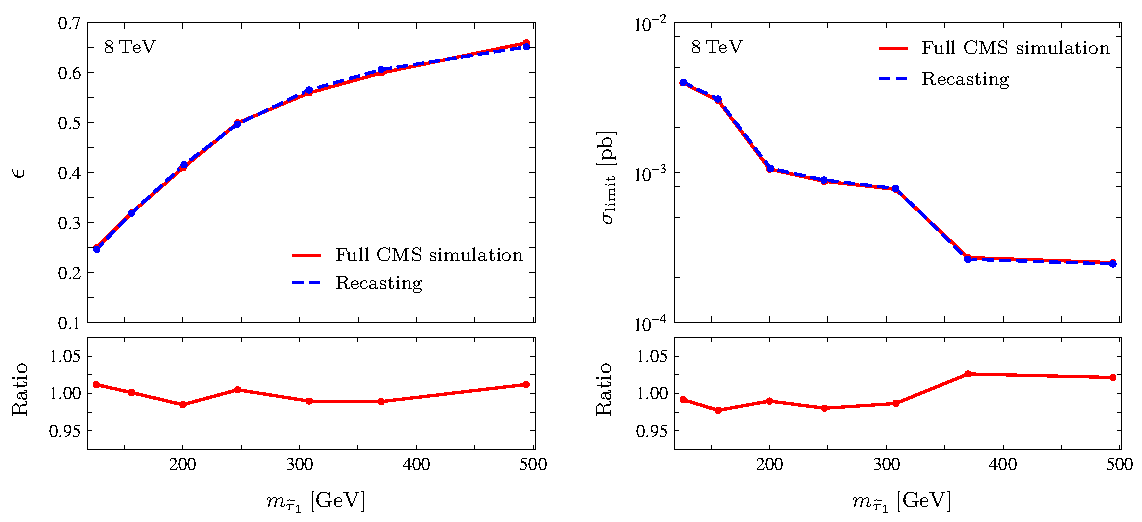
\includegraphics[width=0.99\textwidth]{ch5-figures/HSCP_validation.pdf}}
\end{picture}
\caption{
{\bf{Left: }}Resulting signal efficiency $\epsilon$. {\bf{Right: }}95\% CL cross section upper limit
for the GMSB model as the function of the stau mass. 
We compare the CMS analysis~\cite{Khachatryan:2015lla}
from the full detector simulation (red solid
lines) with the recasting using signature efficiencies (blue dashed lines).
In the lower frames we show the respective ratios
$\epsilon^\text{Full}/\epsilon^\text{Recast}$,
$\sigma^\text{Full}_\text{limit}/\sigma_\text{limit}^\text{Recast}$.
Taken from~\cite{Heisig:2015yla}.
}
\label{fig:gmsbComp}
\end{figure}
%                                      \         |
%                                        \       |s
%                                          \     |
%=====================


Due to the inclusive nature of the search, the above recasting provides 
a widely applicable and highly reliable way to reinterpret the HSCP search for arbitrary 
models containing detector-stable HSCPs. Accordingly it has been used
in a variety of phenomenological studies. For instance, 
it has been used for reinterpretations in
supersymmetric models~\cite{Evans:2016zau,Bagnaschi:2016afc,Heisig:2017lik} and
non-supersymmetric models of very weakly interacting dark matter~\cite{Hessler:2016kwm, Garny:2017rxs}.
In~\cite{Garny:2017rxs} the recasting has been used to reinterpret the HSCP search
for finite lifetimes by convoluting the signature efficiency with the fraction of HSCPs 
that decay after traversing the relevant parts of the detector.
The recasting has also been used for a reinterpretation
in terms of simplified models, as discussed in Sec.~\ref{sec:ch5-smsHSCP}.


%----------------------------------------------------------------------------------------------------------------
\subsubsection{Extrapolation to 13\,TeV} \label{sec:extra}
%----------------------------------------------------------------------------------------------------------------

While the CMS search for HSCPs at 8\,TeV has provided the
signature efficiencies discussed above, the same is not true for
the  13\,TeV analysis~\cite{CMS:2016ybj}.
Therefore a straightforward recasting of the run 2 search is not possible.
Nonetheless, since the 8\,TeV CMS search has proven to be extremely useful
in constraining models with long-lived charged particles,
it would be desirable to recast the 13\,TeV analysis as well.
In the following we discuss an attempt~\cite{inprep2017} 
to obtain a similar recasting for the respective HSCP search at 13\,TeV.
Our aim is to extrapolate the public 8\,TeV efficiencies for the 13\,TeV run by
introducing a correction function $F$ that accounts for the differences between both runs:
\begin{equation}
\label{eq:introF}
P^{13\,\text{TeV}}_{\text{off}}(\vec{k}) = F(\beta) \times
P^{8\,\text{TeV}}_{\text{off}}(\vec{k})\,,
\end{equation}
where we have assumed that the correction function is mainly dependent on the
HSCP velocity. If $F(\beta)$ is sufficient to account for the difference
between both runs and can be computed, we can directly obtain
$P^{13\,\text{TeV}}_{\text{off}}$ and, using the procedure described in
Sec.~\ref{sec:signatureeff}, recast the 13\,TeV analysis.


In order to compute the correction function $F(\beta)$ we use
the total signal efficiencies reported by the  
13\,TeV CMS analysis~\cite{CMS:2016ybj} for
direct production of long lived staus. 
Since the signal efficiencies have been provided for six distinct
values of the stau mass, we perform a fit of $F$ to the efficiencies reported.
We chose to parametrize the correction function $F(\beta)$  by eight parameters
($C_{i}$).
Using  {\sc MadGraph5\_aMC@NLO}~\cite{Alwall:2014hca}
and  \textsc{Pythia}~6~\cite{Sjostrand:2006za} we obtain generator level events
for each of the stau mass points at $13\,$TeV.
Then, comparing the total signal efficiencies obtained for a given set $C_{i}$
to the efficiencies reported in Ref.~\cite{CMS:2016ybj}, we can determine
the best-fit values for the $C_{i}$ parameters and consequently the
best-fit for the correction function ($F_\text{best-fit}$).
The result of the best-fit function and its $1\sigma$ uncertatinty is shown in
Fig.~\ref{fig:F}. The deviation of $F$ from 1 implies a decrease or increase
of the respective detector and signal efficiency between the 8 and 13\,TeV
analyses.  The Figure also shows that the function is loosely constrained
for low values of $\beta$.


%=====================
%    \                                           |
%      \                                         |
%        \                                       |
\begin{figure}[h]
\centering
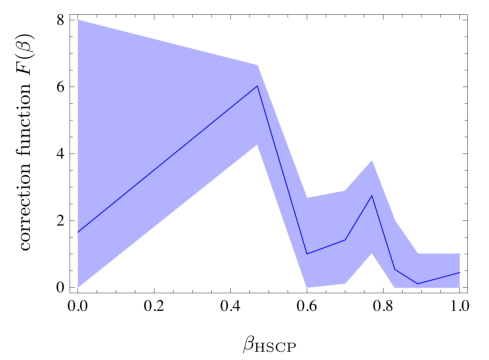
\includegraphics[width=0.7\textwidth]{ch5-figures/HSCP_13TeV_fitB.pdf}
\caption{Best-fit correction function $F(\beta)$ and its $ \pm 1\sigma$ band.
}
\label{fig:F}
\end{figure}
%                                      \         |
%                                        \       |
%                                          \     |
%=====================


In order to verify the validity of the extrapolation to 13\,TeV,
we use $F_\text{best-fit}$ and eq.~\ref{eq:introF} to compute the total signal
efficiencies for the same six benchmark points used in the fit. A comparison
between the results obtained through recasting and the efficiencies reported by
CMS is shown by the second and third columns in Table~\ref{tab:eff}.
The results reproduces the CMS values well within the expected uncertainties,
thus validating the fitting procedure.
Furthermore, the inclusion of the correction function significantly improves the
agreement with respect to the direct extrapolation of the 8\,TeV
efficiencies ($F=1$), as shown by the forth column in Table~\ref{tab:eff}.



\begin{table}[h]
\footnotesize
 % \renewcommand{\arraystretch}{1.2}
 \renewcommand{\arraystretch}{0.5}
 \begin{center}
\begin{tabular}{c|ccc}
 & \multicolumn{3}{c}{direct production } \\
$m_\text{HSCP}$ [{\rm GeV}] & \,$\epsilon(\text{CMS})$ & $\epsilon(F_\text{best-fit})$& $\epsilon(F=1)$ \\
\hline
200   & \,0.235 & 0.232 & 0.259  \\
308   & \,0.294 & 0.298  & 0.346  \\
494    & \,0.387 & 0.384  & 0.452  \\ 
651  & \,0.450  & 0.448   & 0.503 \\
1029 & \,0.497 & 0.501  & 0.466 \\
1599 & \,0.428 & 0.429  & 0.225  \\
\hline
\end{tabular} 
\end{center}
\caption{Efficiencies for the 13\,TeV LHC for the six benchmark masses in the direct stau production scenario 
reported by CMS (second column) and obtained through recasting using
$F_\text{best-fit}$ and without the inclusion of the correction function ($F=1$).}
\label{tab:eff}
\end{table}

The high level of agreement obtained with $F_\text{best-fit}$ 
for the direct stau benchmark points is expected, since these points
were used in order to fit the correction function.
Therefore an independent test of the above fit
must be performed in order to properly validate the recasting of
the 13\,TeV analysis.
Fortunately CMS has also reported efficiencies for a second scenario,
the GMSB model with long lived staus. This scenario not
only contains direct stau production, but also includes production
through cascade decays of heavier sparticles.
Since the GMSB model produces distinct event topologies, it 
provides a good test for the validity of the recasting
procedure.

The results for the six GMSB bechmark points considered in
Ref.~\cite{CMS:2016ybj} are shown in Table~\ref{tab:effGMSB}. As we can
see, they deviate from the CMS values by up to 20\% for large
stau masses, where our estimate undershoots the CMS efficiencies.
Although the overall agreement is improved by the correction function,
the result is not entirely satisfactory, given that 
the uncertainties for the 8\,TeV recasting were
under 5\% (see Fig.~\ref{fig:gmsbComp}).
The observed difference might arise from several shortcomings in our description.
In particular, we assume $F$ to only dependent on $\beta$ whereas the full
probability maps are parametrized in the three kinematic variables $\beta, \eta$ and $p_\text{T}$. 
However assuming a dependence of all three kinematic variables is clearly
not feasible given the very limited amount of information provided by the
13\,TeV CMS analysis.
Therefore we conclude that it is not possible
to extrapolate the 8\,TeV efficiencies in a straighforward way without
additional information from the experimental collaboration.

\begin{table}[h]
\footnotesize
 % \renewcommand{\arraystretch}{1.2}
 \renewcommand{\arraystretch}{0.5}
 \begin{center}
\begin{tabular}{c|ccc}
 & \multicolumn{3}{c}{ GMSB } \\
$m_\text{HSCP}$ [{\rm GeV}] & \,$\epsilon(\text{CMS})$ & $\epsilon(F_\text{best-fit})$& $\epsilon(F=1)$ \\
\hline
200     &\,0.276   & 0.297  & 0.279 \\
308   & \, 0.429 &  0.401 & 0.423  \\
494    & \,0.569 & 0.494 & 0.556  \\ 
651  &  \,0.628 & 0.524 & 0.580 \\
1029 &\,0.665  & 0.538  & 0.493\\
1599 &  \,0.481  & 0.442  & 0.228 \\
\hline
\end{tabular} 
\end{center}
\caption{Efficiencies for the 13\,TeV LHC for the six GMSB model benchmark
points reported by CMS (second column)
and obtained through recasting using $F_\text{best-fit}$ and without the inclusion of the correction function ($F=1$).}
\label{tab:effGMSB}
\end{table}

\vskip 0.1in
\noindent {\bf Lessons learned}
\vskip 0.1in
The prominent signature of HSCPs allows for a mostly inclusive search strategy concentrating
on the HSCP track itself. Hence, searches for HSCPs can be recasted by the use of signature 
efficiencies in a widely applicable and highly reliable way. This possibility has been followed 
by the CMS Collaboration providing signature 
efficiency maps for the 8\,TeV LHC\@. The validation reveals an excellent performance. The
recasting has been successfully used in the literature.
The signature efficiencies for 8\,TeV can also be used to estimate the ones for the 13\,TeV run by applying
a multiplicative correction function. While such an extrapolation introduces some level of approximation
a better knowledge of the underlying changes between both runs might reduce the uncertainties.

%% ################################################ %%

\subsection{Displaced Leptons} 
\label{sec:ch5-displacedLeptons}

Searching for displaced leptons by requiring these to have large impact parameters with respect to the primary vertex is a very clean strategy, and these searches are usually very straightforward to recast. 
The CMS displaced $e\mu$ search~\cite{Khachatryan:2014mea} demands two
oppositely charged, different flavour ($e ,\mu$) leptons with large impact
parameters and it is fairly straightforward to recast. The biggest difficulty
in doing so is locating all of the relevant information, as it is not all
provided within the main document. The ``standard'' isolation requirements used
in the search can be found in an earlier version of the
search~\cite{CMS:2014bra}.
The necessary cuts on the displaced decay position ($v_{T},v_{Z}$) as well as
the invaluable selection (as a function of $p_T$), reconstruction (as a function
of impact parameter, $d_0$) and trigger efficiencies can be found on an
additional website~\cite{CMSemuEfficiency} containing auxiliary information for
recasting.  Although all of this information is excellent and greatly
facilitates recasting the search, the fact that the additional material is not
referenced in the document makes rounding up the information challenging.

\begin{table}%
\centering
\parbox{0.4\textwidth}{
\begin{footnotesize}
\begin{tabular}{| c |} \hline
{\bf Cut Summary of CMS displaced $e\mu$}    \\ \hline \hline
{\bf Preselection}    \\ \hline
{1 OS $e^\pm\mu^\mp$ pair} \\  
{$d_\ell>100\,\mu$m} \\
{$p_{T,\ell}>25$ GeV,  $ \left\vert \eta_\ell \right\vert <2.5$} \\  
{Reject $1.44 <  \left\vert \eta_e \right\vert<1.56$} \\  
{$I^{calo,e}_{\Delta R<0.3}<0.10$}, {$I^{calo,\mu}_{\Delta R<0.4}<0.12$} \\  
{ $\Delta R_{\ell j}>0.5\; \forall$ jets with $p_T>10$ GeV } \\
{$\Delta R_{e\mu}>0.5$} \\
{$v_{T,\tilde \ell} < 4 \,\mbox{cm}$, $ v_{Z,\tilde \ell} <  30 \,\mbox{cm}$}\\
{Veto additional leptons} \\
 \hline 
\end{tabular}
\end{footnotesize}
% \label{tab:cuts}
}
\qquad
\begin{minipage}[c]{0.45\textwidth}%
\centering
    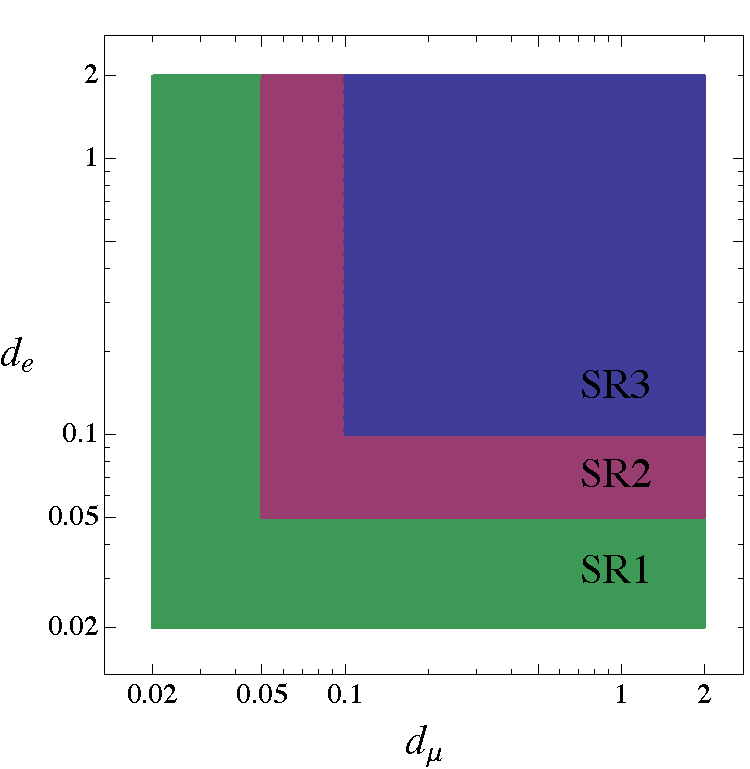
\includegraphics[width=0.9\textwidth,angle=0]{ch5-figures/SRplot.pdf}
\label{tab:cuts}
\caption{{\bf Left:} Preselection cuts in \cite{Khachatryan:2014mea} (see also \cite{CMS:2014bra,CMSemuEfficiency}).  {\bf Right:} the transverse impact parameter bins that define the exclusive signal regions.  Table and figure taken from \cite{Evans:2016zau}.
  \label{tab:cuts}} 
\end{minipage}
\end{table}

\vspace{0.5cm}

The benchmark model used in this search is the direct pair production of stops
that decay through small lepton-flavor-universal RPV $\lambda'_{ijk}L_iQ_jD^c_k$
couplings ($\lambda'_{133}=\lambda'_{233}=\lambda'_{333}$) to yield displaced
$\tilde t \to e b$, $\mu b$, and $\tau b$ decays.  The signal is simple to
generate, the only challenge is in handling the displacement properly. The most
identifying preselection requirement of this search is that the transverse
impact parameter, $d_0$, is required to be larger than 100 $\mu$m for both the
electron and muon.  The impact parameter is not the point where the parent
object (e.g., $\tau$ or $b$) decays, i.e., the $v$ mentioned above, but the
distance to the point of closest approach for the lepton's track relative to the
center of the beampipe.  Backgrounds in this search from $Z\to\tau\tau$ or heavy
flavor tend to result in leptons that are nearly collinear with the parent due
to the small mass-to-momentum ratio, and yield a small impact parameter even for
decays well on the lifetime tail of the parent.  Events are binned across three
exclusive signal regions: SR3, where both leptons have transverse impact
parameters $d_e$ and $d_\mu$ between $0.1$ and $2.0$ cm; SR2, with $d_e$ and
$d_\mu$ between $0.05$ and $2.0$ cm, but not satisfying the requirement of SR3;
and SR1, with $d_e$ and $d_\mu$ between $0.02$ and $2.0$ cm, but not within SR2
or SR3.  All selection requirements are summarized in Table~\ref{tab:cuts}.
 
\begin{figure}[ht]
\begin{center}
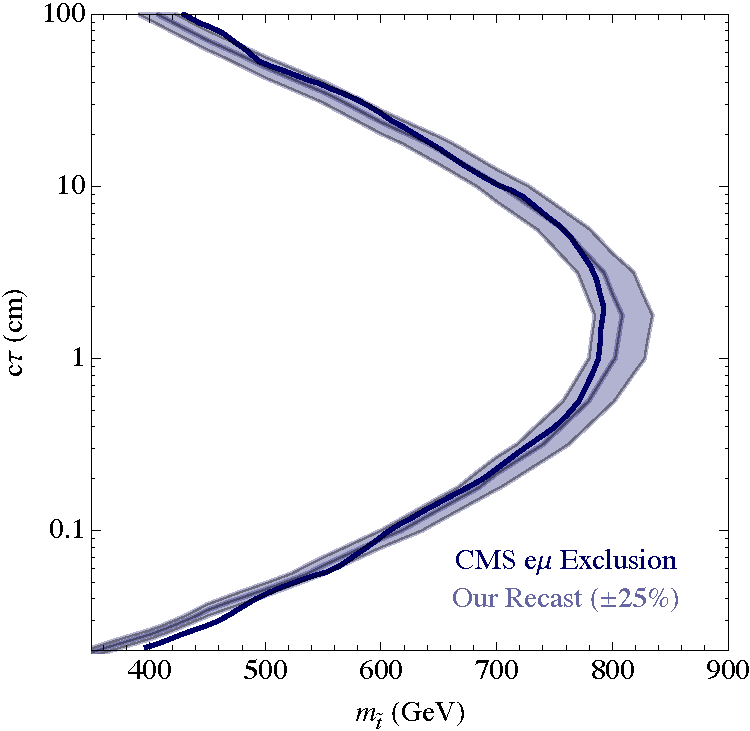
\includegraphics[width=0.45\textwidth,angle=0]{ch5-figures/emuVal.pdf}
\end{center}
\caption{Validation of the CMS displaced $e\mu$ search~\cite{Khachatryan:2014mea} for
  the displaced supersymmetry benchmark model
  \cite{Graham:2012th}.  Figure taken from \cite{Evans:2016zau}.
}
\label{fig:DTval}
\end{figure}

In Figure~\ref{fig:DTval}, we present the validation of the CMS displaced $e\mu$
search~\cite{Khachatryan:2014mea} from the study performed
in~\cite{Evans:2016zau}.  For this search, we show the recommended 25\% modeling
uncertainty. The recast agrees very well with the results from the CMS displaced
$e\mu$ search  in the region of highest sensitivity, 300 $\mu$m $\lesssim c\tau
\lesssim 50$ cm, but exhibits a moderate deviation on the tails.   As this
extremely low efficiency region is overly sensitive to the tails of the
distribution, it may be the case that the sensitivity is slightly underestimated
for lifetimes near 1 m or 100 $\mu$m, but this discrepancy typically has no
qualitative impact on any application of the results.

\subsubsection{Extrapolation to 13 TeV}

We now show another reinterpretation example of the CMS displaced $e\mu$ in
order to highlight the comparison between 8~\cite{Khachatryan:2014mea} and 13
TeV~\cite{CMS-PAS-EXO-16-022} analyses. We compare in
Figure~\ref{fig:ch5-valid1} our reproduction of expected signal events with the
published validation material for the 8 TeV version, and the partially-available
validation material for the 13 TeV search.
Information on efficiency maps from the 8 TeV analysis was needed
to obtain an extrapolation to 13 TeV, as the 13 TeV maps are not yet public.
As we can see, the 8 TeV recast for the CMS displaced lepton
search~\cite{Khachatryan:2014mea} agrees very well in the region of highest
sensitivity. The 13 TeV recasting, however, underestimates the CMS values
by a factor of two or more. This is likely due to the fact that the
lepton efficiencies can not be directly extrapolated from 8 to 13 TeV,
as assumed in Figure~\ref{fig:ch5-valid1}. 
Also, with the absence of a cutflow table, it is impossible to verify where the
mismatch arises: if it is due to mis-modelling of the signal region
cuts or indeed due to changes in the efficiencies.



\begin{figure}[ht]
\centering
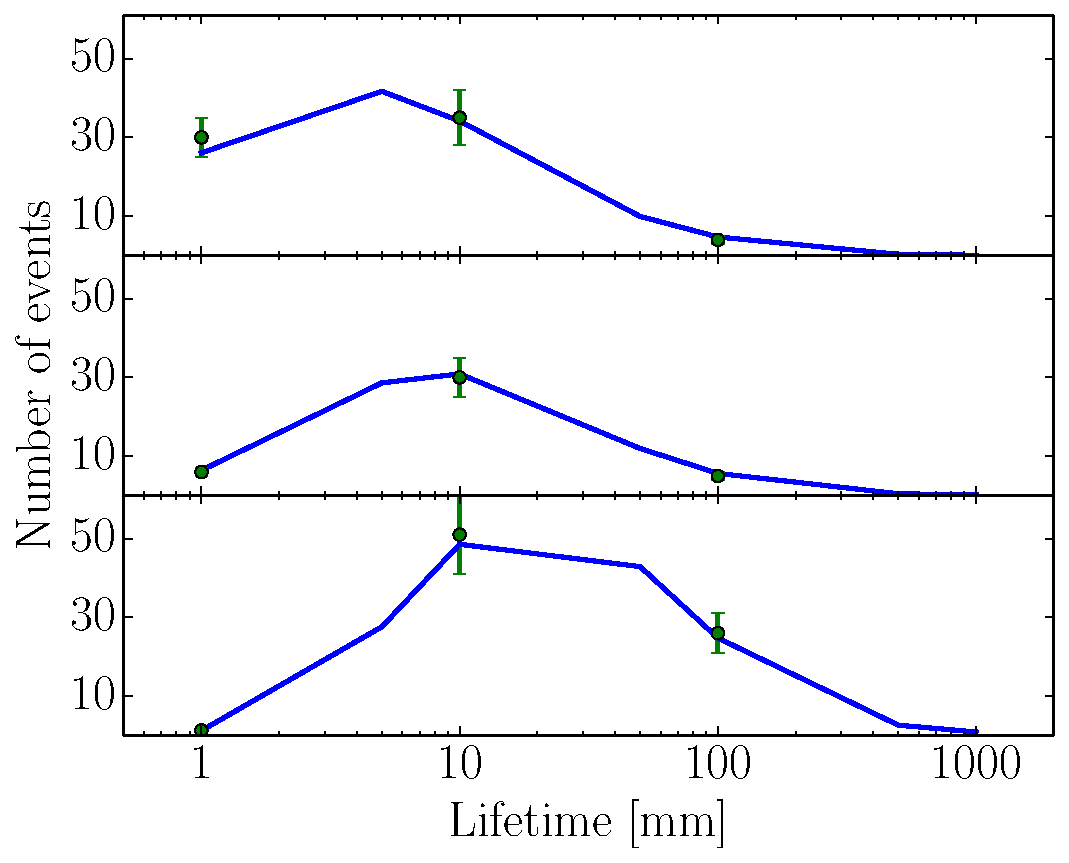
\includegraphics[width=0.45\textwidth,angle=0]{ch5-figures/disp_lep_8tev.pdf}
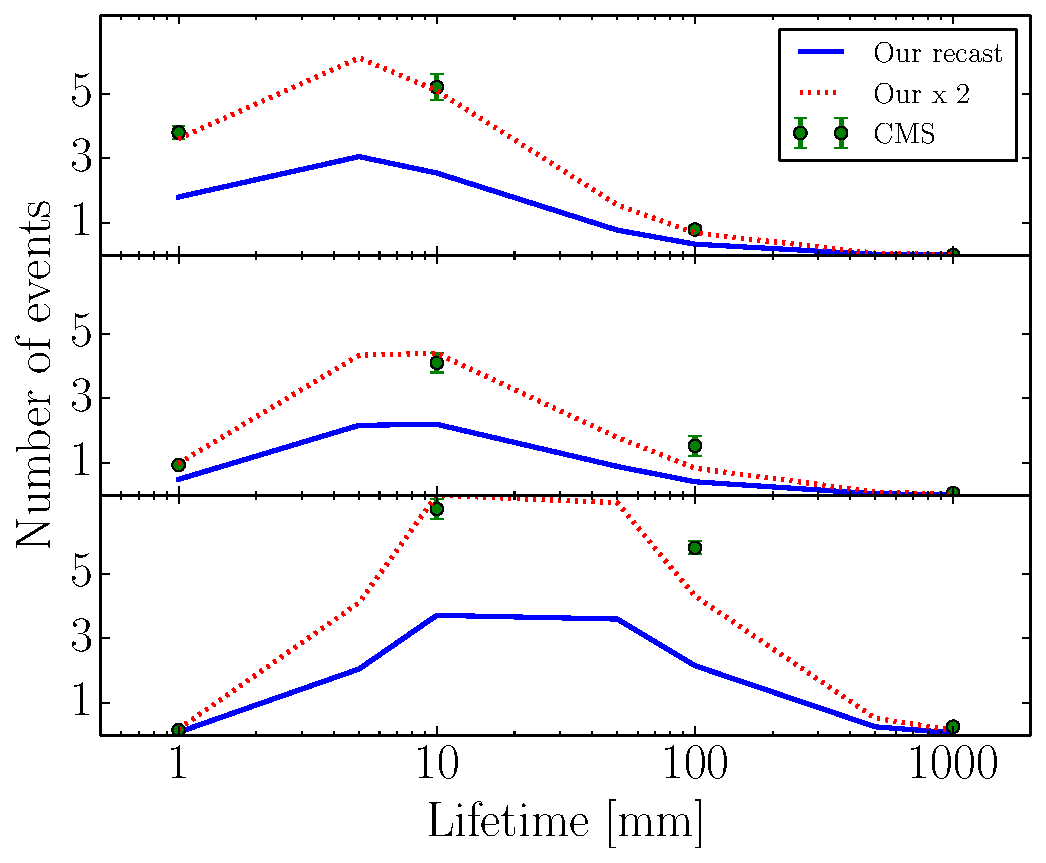
\includegraphics[width=0.45\textwidth,angle=0]{ch5-figures/disp_lep_13tev.pdf}


\caption{\label{fig:ch5-valid1} Number of expected events in the signal regions defined based on $d_0$.  The green points refer to the expected signal published by the analysis. {\bf Left:} Validation for 8 TeV analysis.  Production cross section assumed NLO+NLL value 85.6 fb for $M_{\tilde t_1} = 500$ GeV, BR = 0.33 in each $\ell$-channel. {\bf Right:} Validation for 13 TeV analysis. Production cross section assumed NLO+NLL value 67.0 fb for $M_{\tilde t_1} = 700$ GeV. The 13 TeV numbers are made using efficiency maps published for the 8 TeV search, as the 13 TeV maps are not yet public. Figures taken from~\cite{LesHouches2017}.}
\end{figure}

\vskip 0.1in
\noindent {\bf Lessons learned} 
\vskip 0.1in

The selection and trigger efficiencies provided by CMS
are very useful for recasting the 8 TeV CMS search for
displaced leptons~\cite{Khachatryan:2014mea}
and allow for a very good level of agreement.
The main challenge, however, consisted in collecting all the available
information, which was not provided by the main document in
Ref.~\cite{Khachatryan:2014mea}.
Furthermore, the corresponding information for the 13 TeV search is
not publicly available and an extrapolation of the 8 TeV efficiencies
was shown to be inadequate.

\subsection{Displaced Jets}
\label{displacedJets}

Searches for displaced jets are less straightforward to reinterpret than
displaced leptons. Interest in accurate reinterpretation is increasing, as many
new physics models are sensitive to this particular signature. The work
in~\cite{Cui:2014twa} explores long-lived particle (LLP) signatures for certain
weak-scale models of baryogenesis~\cite{Cui:2012jh,Cui:2013bta,Cui:2014twa},
where the CMS search for displaced dijets~\cite{CMS-PAS-EXO-12-038} was
reinterpreted.

This search uses a multivariate discriminant composed of observables that are
challenging to model in Monte Carlo (MC), such as the track vertex multiplicity
and the root-mean-square of a cluster track multiplicity variable. The
reinterpretation approach in Ref.~\cite{Cui:2014twa} was to construct track
information at truth level based on the output of a parton shower program (such
as {\sc{Pythia 8}}), and then use the truth-level information to construct the
various vertex, cluster, and track-level observables for each event. As it is
difficult to adequately account for inefficiencies of track and vertex
reconstruction, the efficiency of passing the cuts with truth-level observables
was considered and then it was normalized to the results from CMS. To do so, we
simulated identical signal models to those with efficiencies reported by the CMS
collaboration, assumed that the MC truth-level reconstruction gave an adequate
description of kinematics but \emph{not} track and vertex reconstruction, and so
computed a ratio of truth-level efficiencies to those reported by CMS. Then we
use these efficiency ratios to re-scale the truth-level results of other models,
leading to a reinterpretation of the CMS search for different models beyond the
ones they considered. The details can be found in Ref.~\cite{Cui:2014twa}.

To validate this approach, truth-level quantities for the models constrained in
Ref.~\cite{CMS-PAS-EXO-12-038} were computed and compared to the numbers and
distributions reported in Ref.~\cite{CMS-PAS-EXO-12-038} [\textcolor{red}{These are the same reference.}]. For example,
comparisons of the distributions of the observables going into the multivariate
discriminant, as well as the output of the multivariate discriminant could be
performed. While the truth-level distributions disagreed with those of CMS for
individual observables, the actual multivariate discriminant output agreed with
that of CMS at better than 25\%. The ratio of truth-level efficiencies to CMS
efficiencies are also compared for different LLP masses and kinematics, and
these typically agree with one another at the factor-of-two
level~\cite{Cui:2014twa}. This suggests that this reinterpretation of the CMS
results in terms of cross-section limits is likely accurate to the factor-of-two level.

\vskip 0.1in
\noindent {\bf Lessons learned}
\vskip 0.1in

We find that a rather na\"ive truth-level reconstruction of the event could give a reinterpretation of cross-section limits to agree within a factor of two, provided the efficiencies were normalized to the experimental values using an overlapping set of signal models. One of the major obstructions to improving on the accuracy of the estimate was the model-dependence observed among the ratios of efficiencies. For instance, it was found that highly boosted models showed a much lower relative reconstruction rate in data vs.~truth-level MC. Since pair production of LLPs was considered near threshold, this degradation in the performance of highly boosted LLPs is not particularly troubling. However, it does suggest that characterizing the effects of the particle boost are important for reinterpretation.

In addition, with a larger and more diverse set of signal benchmarks available, the prospects for the reinterpretation of search results are better. The reasons are twofold:~
%
\begin{itemize}
\item Increasing the number of presented signal models by the collaboration allows for more cross-checks between MC and the results in data. This allows for more sophisticated tuning of models;
\item Having a more diverse set of benchmark signal models means that it is easier to dis-entangle various kinematic effects on the efficiency (such as the LLP mass, boost, etc.) and find a signal benchmark that most closely matches the model for which one wants to derive a limit.
\end{itemize}
%

\subsection{Displaced Lepton-Jets}

\red{GC: Will include recast later, Michael agreed to contribute to this, awaiting for input.}


\subsection{Non-pointing Photons}

The search for non-pointing photons produced in association with missing
transverse energy ($\slashed E_T$)~\cite{Aad:2014gfa} plays an important role in probing beyond-the-SM (BSM) particles that decay to a SM photon and an invisible particle through a highly suppressed coupling. Beside the gauge-mediated supersymmetry breaking (GMSB) models~\cite{Dine:1981gu}, which were the main motivation for the non-pointing photon search, this type of signal can also appear in many hidden sector models. For example, in the dipole-mediated DM model (the Dark Penguin)~\cite{Primulando:2015lfa}, the production of two heavier dark fermions $pp\to Z^*/\gamma^*\to\chi_h\bar{\chi}_h$ is followed by the decays $\chi_h \to \chi_l+ \gamma$. If the flavor structures of the DM mass and coupling are aligned, $\chi_h$ can be long-lived and give rise to non-pointing photons. Another example is provided by the dark shower scenario~\cite{Freytsis:2014sua,Freytsis:2016dgf} that explains the galactic center gamma-ray excess. In this model, many hidden pions can be produced in the same LHC event. Some of these have displaced decays to a pair of SM photons, while others decay outside of the detector, yielding $\slashed E_T$. Notice that in this case the topology of the events is different from the previous examples, as the non-pointing photons and $\slashed E_T$ originate from separate particles.

In this note we describe a method to recast the bounds of
Ref.~\cite{Aad:2014gfa} to a BSM scenario that is different from the GMSB model,
using the Dark Penguin signal \cite{Primulando:2015lfa} as example.

\begin{figure}
\begin{center}
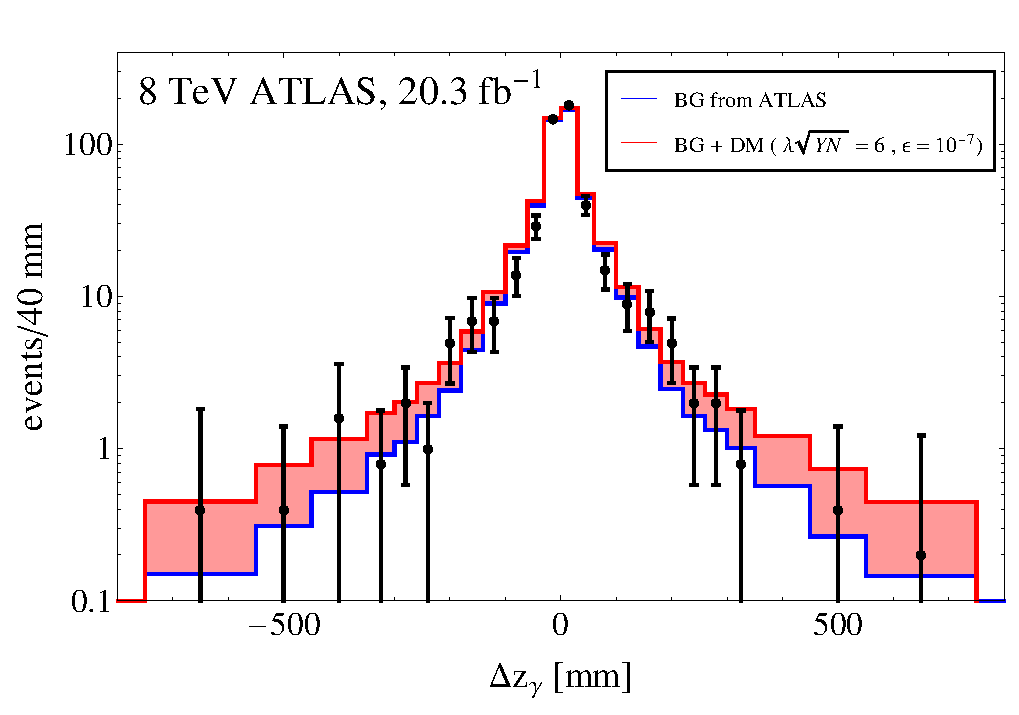
\includegraphics[width=0.45\textwidth]{ch5-figures/nonpointing_photon}\qquad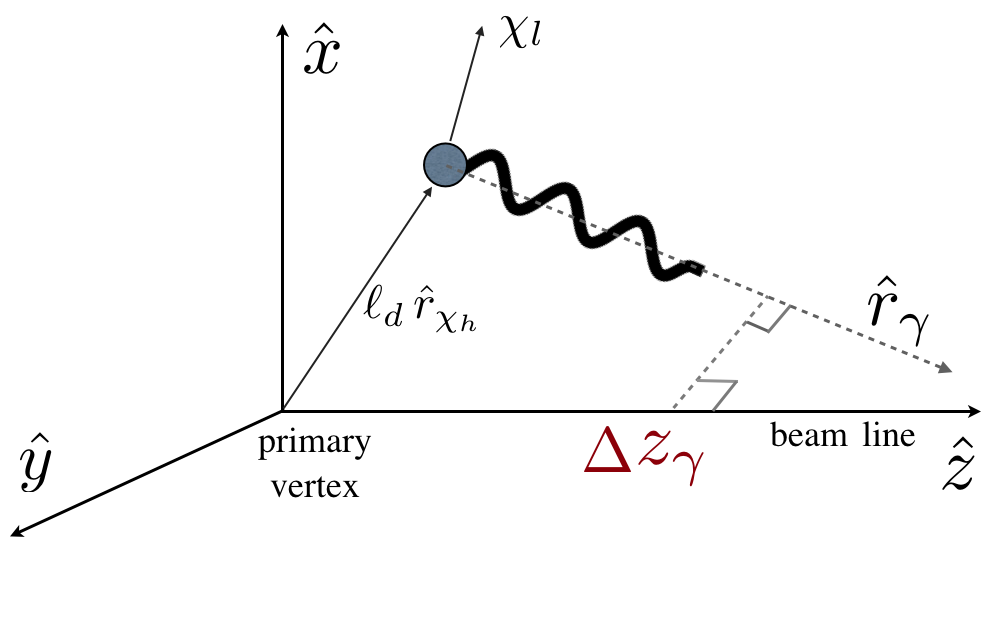
\includegraphics[width=0.45\textwidth]{ch5-figures/displaced_cartoon}
\end{center}
\caption{{\bf {Left}}: the $\Delta z_{\gamma}$ distribution of the non-pointing photon signals measured by ATLAS. The background reported by ATLAS (blue histogram) was obtained from a data-driven analysis, using diphoton events with $\slashed E_T<20$ GeV. Also shown, stacked on top of the background (red histogram), is the signal distribution from the dipole-mediated DM scenario with $(m_{\chi_h},\,m_{\chi_l},\,M)=(300,\,10,\,300)$ GeV, $\lambda\sqrt{NY}=6$, and $\varepsilon=10^{-7}$. See Ref.~\cite{Primulando:2015lfa} for more details. {\bf{Right}}: the geometry of the displaced signals.}
\label{fig:nonpointing}
\end{figure}

%%%%%%%%
\subsubsection{Calculation of the signal efficiency for the non-pointing photon search}
%
We follow the non-pointing photon analysis in Ref.~\cite{Aad:2014gfa}, performed
by the ATLAS collaboration on about $20$ fb$^{-1}$ of $8$ TeV data. In
Ref.~\cite{Aad:2014gfa} delayed photons were also considered, but here we focus
only on the measurement of the $\Delta z_{\gamma}$ of non-pointing photons (see
Fig.~\ref{fig:nonpointing}). For DM signals given by the long-lived
$\chi_h\to\chi_l\gamma$ decay, $\Delta z_{\gamma}$ can be related to the
$\chi_h$ decay length $\ell_{d}$ in the lab frame:
\begin{equation}\label{eq:Zgamma}
\Delta z_{\gamma}=\ell_d\left(\hat{r}_{\chi_h,z}-\frac{\hat{r}_{\chi_h,T}\cdot\hat{r}_{\gamma,T}}{1-(\hat{r}_{\gamma,z})^2}\hat{r}_{\gamma,z}\right) = \ell_d \Big[\cos\theta_{\chi_h} -\cos (\phi_{\chi_h} - \phi_\gamma)\mathrm{cot}\,\theta_\gamma \sin \theta_{\chi_h} \Big]
\end{equation}
where $\hat{r}_{T,z}$ represent the transverse and longitudinal components of
the unit vector $\hat{r}$, respectively, as shown in Fig.~\ref{fig:nonpointing}.
To obtain the $\Delta z_{\gamma}$ distribution of the DM decay, we first
simulate the prompt process, $p\,p \to \chi_h\bar{\chi}_h,
\chi_h\to\chi_l\gamma, \bar{\chi}_h\to\bar{\chi}_l\gamma$ in MadGraph5, then we
apply the cuts performed in the ATLAS analysis, and finally reweight the events
using the dark penguin form factors. Then we calculate the proper lifetime of
$\chi_h$ and boost it to the lab frame using the momenta of each parton-level
event. The angular information of the photon and $\chi_h$ allow us to calculate
$\Delta z_{\gamma}$ in Eq.~\eqref{eq:Zgamma} as a function of the decay length.
Using this, each simulated MC event contributes to the differential cross
section in $\Delta z_{\gamma}$ as
\begin{equation} \label{eq:displdistr}
\frac{d\sigma_{\text{displaced}}}{d\Delta z_{\gamma}} =\sigma_{\text{prompt}}\frac{d\,P}{d\Delta z_{\gamma}}=\sigma_{\text{prompt}}\frac{|\mu|}{2} e^{-\mu\,\Delta z_{\gamma}},
\end{equation}
where the $\mu$ characterizing the probability distribution $dP/d\Delta z_\gamma$ of the decay is defined as
\begin{equation}
\mu\equiv\frac{\Gamma_{\chi_h}m_{\chi_h}}{p_{\chi_h}}\left(\hat{r}_{\chi_h,z}-\frac{\hat{r}_{\chi_h,T}\cdot\hat{r}_{\gamma,T}}{1-(\hat{r}_{\gamma,z})^2}\hat{r}_{\gamma,z}\right)^{-1}.
\end{equation}
Summing the distributions derived from all the simulated events we obtain the
differential cross section in $\Delta z_\gamma$, see Fig.~\ref{fig:nonpointing}.

The ATLAS search requires at least two loose photons with $|\eta|<2.37$ and $E_T>50$ GeV. At least one photon is required to be in the barrel region $|\eta|<1.37$. To avoid collisions due to satellite bunches, both photons are required to have an arrival time at the ECAL $t_{\gamma}$ smaller than $4$ ns, with zero defined as the expected time of arrival for a prompt photon from the primary vertex. We approximate $t_\gamma$ with the time of flight of the $\chi_h$, requiring it to be smaller than $4$ ns. 
In our estimation we do not include the detailed isolation cuts on the photon. We also neglect the effect of the displaced decay on the angular acceptance of the photons, simply imposing the requirements on $|\eta|$ at the level of the prompt event. 
The signal region also requires $\slashed E_T>75$ GeV. 
Finally, to simplify the discussion we assume that every event has a
reconstructed primary vertex in the geometrical center of the detector.


For events where only one photon satisfies $|\eta|<1.37$ (i.e. it is in the
barrel calorimeter), this photon is used for the measurement of $\Delta
z_{\gamma}$. For events where both photons are in the barrel, the photon with
larger $t_{\gamma}$ is used. We approximate this timing condition by taking the
photon emitted by the more boosted $\chi_h$, in which case the average decay is
more delayed. In Fig.~\ref{fig:nonpointing} the generated $\Delta z_{\gamma}$ signal distribution is shown, on top of the expected background. The latter is taken from Fig.~4 of the ATLAS paper \cite{Aad:2014gfa}. Because we are focusing on the non-pointing photon signals, to set constraints on the DM couplings in \cite{Primulando:2015lfa} we remove events with $|\Delta z_{\gamma}|< 30$ mm. In our exploratory analysis we only consider the statistical uncertainty on the background, neglecting the effect of systematics.

\vskip 0.1in
\noindent {\bf Lessons learned} 
\vskip 0.1in

The ATLAS paper gives detailed descriptions of the cuts and background analysis, which makes an approximate estimation of the signal efficiency quite straightforward. 

The background analysis in Ref.~\cite{Aad:2014gfa} is based on a data-driven study, for which events passing the diphoton selection with $\slashed E_T<20$ GeV are used as control region sample. It is challenging for theorists to simulate the background for different energy cuts. Especially for the $\slashed E_T$ cut that plays a vital role in the DM and Hidden Valley searches.

In order to obtain a more precise result it would be useful if the ATLAS collaboration could provide the reconstruction efficiency of non-pointing photons as function of $\Delta z_{\gamma}$, or of the angle between the photon and the surface of the ECAL, a variable that may be relevant to the efficiency. The paper does provide a table of signal acceptance times efficiency for the GMSB SPS8 model, but it is not easy to apply those results to different new physics models.

It would also be very useful to have a table of background events for different cuts on $\slashed E_T$. For instance, for the Dark Penguin the typical $\slashed E_T$ from the decay of $\chi_h\bar{\chi}_h$ with electroweak-scale $m_{\chi_h}$ can easily be higher than $100$ GeV. By contrast, in the dark shower scenario where soft hidden pions decay to two SM photons, the $\slashed E_T$ originating from additional late-decaying pions can be much lower than the $75$ GeV cut used in the ATLAS analysis. Knowing the background and systematic uncertainty for different $\slashed E_T$ cuts would be very important to constrain different models.


\subsection{Disappearing Tracks}
\label{sec:ch5-disappearingTracks}

{\color{red}{ZL: Awaiting input from Rakhi Mahbubani}}

\subsection{Displaced Vertices}
\label{sec:ch5-displacedVertices}

Displaced vertex searches differ from displaced jets and displaced leptons ones in the fact that actual reconstruction of a secondary vertex using track information is made. The lifetime of the LLP should allow it to decay either in the inner trackers or
muon spectrometer of the LHC detectors, where vertexing is possible~\cite{Aaboud:2017iio,Aad:2015rba,Aad:2015uaa,CMS:2014wda,CMS:2014hka,Aaij:2016xmb,Aaij:2017mic}. These searches have an extremely low background, as there are no irreducible contributions from the SM, making them sensitive to very small signals of new physics.

In this section we make the distinction when reinterpretation of displaced searches makes use of truth information to identify displaced decays and where an attempt to reconstruct them from displaced tracks is performed (with an approximate detector response).

\subsubsection{Truth Level Displaced Vertices}

The work in~\cite{Cui:2014twa} reinterpreted the 8 TeV ATLAS search for a displaced muon and a multi-track vertex (DV+$\mu$)~\cite{ATLAS-CONF-2013-092}, where long-lived particle signatures for certain weak-scale models of baryogenesis~\cite{Cui:2012jh,Cui:2013bta,Cui:2014twa} where explored. For reinterpreting this search, a similar procedure described in the displaced jets 
section~\ref{displacedJets} of constructing ratios of truth-level vs.~ATLAS efficiencies for the ATLAS multi-track vertex analysis~\cite{ATLAS-CONF-2013-092} was performed, with similar results for the validation being correct within approximately a factor of two. 

This DV+$\mu$ analysis has since been superseded by~\cite{Aad:2015rba}, where a displaced vertex is looked for at 8 TeV in association with either a muon, electrons, jets and missing transverse momenta. Recently, an updated ATLAS paper~\cite{Aaboud:2017iio}, which looks for multi-track displaced vertices at 13 TeV in association with large missing transverse momenta, was made public. This search now includes a prescription using parametrized efficiencies as a function of vertex radial distance, number of tracks and mass. Their prescription can be applied to vertices and events passing certain particle level acceptance requirements using the truth MC event record. 

Here we validate the prescription with parametrized selection efficiencies
in~\cite{Aaboud:2017iio}~\footnote{This prescription is also validated in
Ref.~\cite{LesHouches2017}.}. The results of this search are interpreted by ATLAS in a split SUSY simplified model with a long-lived gluino that hadronizes forming an $R$-hadron before decaying, $\tilde{g}\rightarrow q\bar{q}\tilde{\chi}^{0}_{1}$. Event samples are generated with \textsc{Pythia 8.2}~\cite{Sjostrand:2014zea}. We use truth level missing transverse momenta and we identify the truth $R$-hadron decay position and decay products, as the ATLAS collaboration provides selection efficiencies that can be directly applied to this truth level quantities. These efficiencies can be found in the auxiliary material in~\cite{SUSY-2016-08}, and are given at the event-level as a function of the truth missing transverse momenta and displaced vertex radial distance, and at the vertex level parametrized as function of vertex invariant mass and number of tracks, and are given for different detector regions, encapsulating also the effect of the material veto cut.

The selection of events used for the signal region requires:

\begin{itemize}
\item{truth level missing transverse momenta $>200$ GeV.}
\item{one trackless jet with $p_{T}>70$ GeV, or two trackless jets with $p_{T}>25$ GeV. A trackless jet is defined as a jet with $\sum_{tracks} p_{T}<5$ GeV.}
\end{itemize}

In addition, events must have at least one displaced vertex with:

\begin{itemize}
\item{transverse distance detween the IP and the decay position $>4$ mm.}
\item{the decay position must lie in the fidutial region $r_{DV}<300$ mm and $|z_{DV}|<300$ mm.}
\item{the number of selected decay products must be at least 5, where selected decay products are charged and stable, with $p_{T}>1$ GeV and $|d_{0}|>2$ mm.}
\item{the invariant mass of the truth vertex must be larger than 10 GeV, and is constructed assuming all decay products have the mass of the pion.}
\end{itemize}

Applying these cuts and efficiencies, we get event-level efficiencies for two of
the benchmarks, where the gluino mass is 1400 GeV or 2000 TeV (and the
neutralino mass is fixed to 100 GeV). Based on the efficiencies obtained and the
estimated number of background vertices, we can extract 95\% CL upper limits on
the total visible cross section for the two gluino masses. For reference,
assuming $100\%$ efficiency, we get an upper limit of $0.091$ fb. The
curves in Figure~\ref{fig:DVsigmaLimits} show our recasting results compared to
ATLAS. The level of agreement is very good, within 20\% for most of the
lifetime values. We also point out that the recasting limits agree well
even for regions where the efficiency is very low ($\tau > 10$~ns
and $\tau < 10^{-2}$~ns).

\begin{figure}[t]
\begin{center}
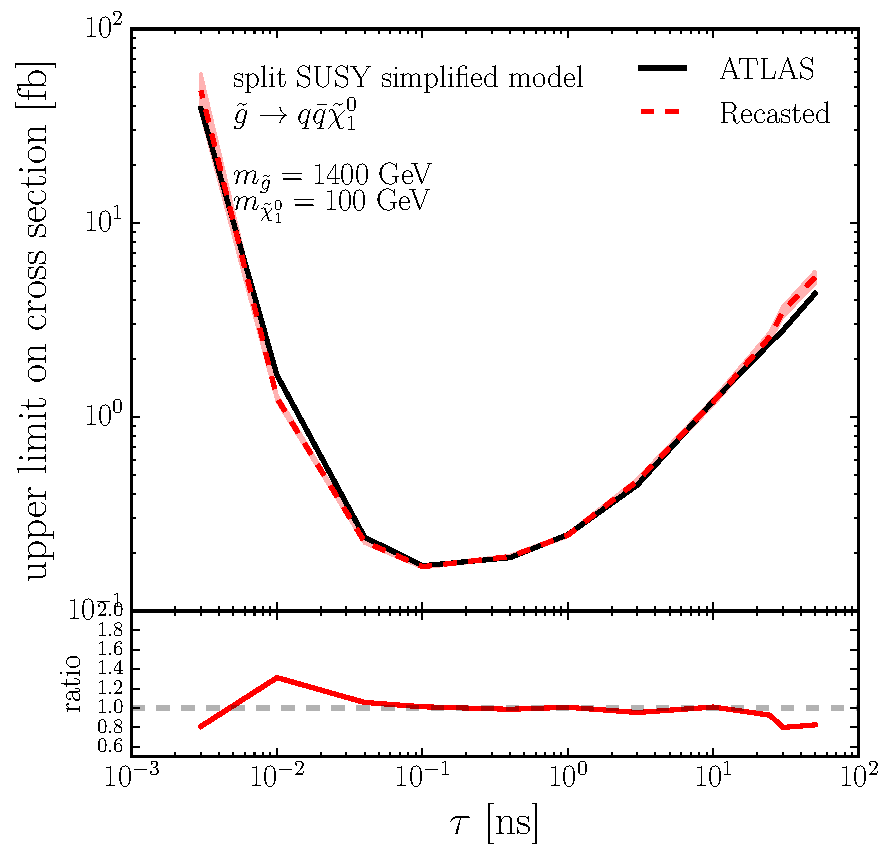
\includegraphics[width=0.45\textwidth]{ch5-figures/limits_gluino1_FIXED.pdf}
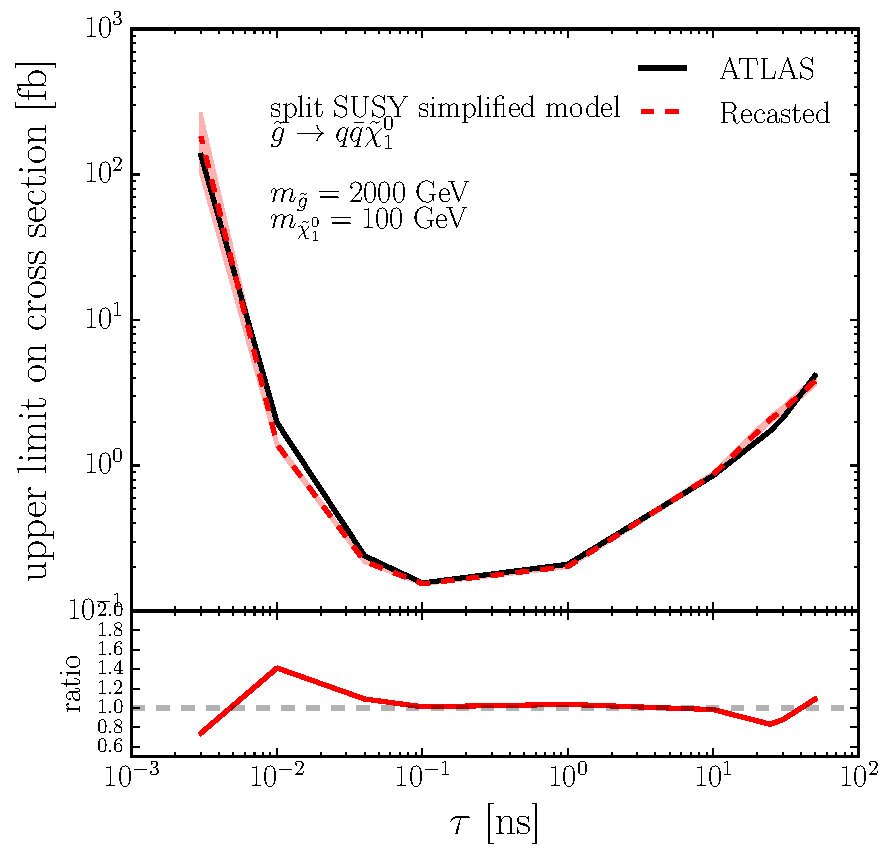
\includegraphics[width=0.45\textwidth]{ch5-figures/limits_gluino2_FIXED.pdf}
\caption{ Comparison of our recast and ATLAS~\cite{Aaboud:2017iio} on the upper limit in the gluino production cross section against its proper lifetime~\cite{LesHouches2017}.}
\label{fig:DVsigmaLimits}
\end{center}
\end{figure}

\subsubsection{Displaced Vertex Reconstruction}

Before parametrized efficiencies applicable for truth-level displaced vertices where made public, attempts to recast displaced vertex searches were made by performing their reconstruction from charged tracks only, with an approximate detector response. In Ref.~\cite{Allanach:2016pam} the ATLAS DV+jets multitrack analysis~\cite{Aad:2015rba} was recasted. Reinterpretation was performed using generator-level events and the detector fiducial region was reproduced as well as possible.  The jets are clustered according to the anti-kt prescription in the analysis with momentum smearing (this is validated by reproducing the jets+MET exclusion curve of prompt searches).  The selection of events used for the signal region (and the approximations to real detector simulation) were as follows:

\begin{table}[ht] 
\footnotesize
\begin{center}
% \begin{tabular}{|p{3.0cm}p{12.5cm}|}
\begin{tabular}{|p{2.0cm}p{7cm}|}
\hline
{ DV jets}     & 4 or 5 or 6 jets with  $|\eta| <2.8$ and $p_{T} > 90, 65,
55$ GeV, each\\ 
 & \\
{ DV reconstruction}$^*$   & DV made from tracks with $p_{T}>1$ GeV, $|\eta|<2.5$ and $|d_{0}|>2$ mm. Vertices within 1 mm are merged. Note: a tracking efficiency needed here; we assume a functional form given by equation~\ref{eqn:trkeff} \\
 & \\
{  DV fiducial}         & DV within $4$ mm $<r_{DV}<300$ mm and $|z_{DV}|<300$ mm
\\  
 & \\
{ DV material}$^*$         & No DV in regions near beampipe or within pixel layers. Discard tracks with $r_{DV}/\mathrm{mm} \in \{[25,38], [45,60], [85,95], [120,130]\}$.\\ 
                    & \\
                    & \\
 $N_{\rm trk}$       & DV track multiplicity $\geq 5$ \\
 & \\
  $m_{DV} $         & DV mass $>10$ GeV \\
\hline 
\end{tabular}
\end{center}
\caption{\label{tab:cutflow_ATLAS} Implementation of cuts applied in the ATLAS
  multitrack DV + jets search, from Ref.~\cite{Aad:2015rba}. $^*$ These are approximations to the experimental analysis in the absence of the full detector simulation. }
\end{table}

A tracking efficiency of the form

\begin{equation}
\scriptsize
\varepsilon_\mathrm{trk} = 0.5\times \left(1-\exp\left(\frac{-p_{T}}{4.0\mathrm{~GeV}}\right)\right)  \times\exp\left(\frac{-z_\mathrm{DV}}{270\mathrm{~mm}}\right)  \times \mathrm{max}(-0.0022\times{\frac{r_\mathrm{DV}}{\mathrm{1\mathrm{~mm}}}}+0.8,0),
\label{eqn:trkeff}
\end{equation}


is used, where $r_\mathrm{DV}$ and $z_\mathrm{DV}$ are the transverse and longitudinal distance of the track's production vertex (same as displaced vertex origin when using truth-level generator information).  This functional form is designed to take into account the size of the detector (linear dependence on $r_\mathrm{DV}$, exponential on $z_\mathrm{DV}$), as well as a turn-on like feature dependent on the $p_{T}$ of the track. It reproduces the overall behavior of efficiency falling off with vertex displacement. The parameters were determined by fitting the efficiency curve (with lifetime dependence), for three benchmarks in the analyses.  We find that fitting only one benchmark does not correctly reproduce the efficiency curve for any of the others.  This is most likely due to insufficient dimensionality of the efficiency map.  We expect that a full tracking efficiency parametrisation depends not only on $r_\mathrm{DV}$, $z_\mathrm{DV}$ and $p_T$, but also transverse and longitudinal impact parameters ($d_0$,$z_0$), and on charge and pseudorapidity of the track. Furthermore, we expect a vertex efficiency that depends on the topology of the event and the nature of the particles forming the vertex. The fit for the event efficiencies from this tracking function can be seen in Figure~\ref{fig:trkeff}.

\begin{figure}[h]
\begin{center}
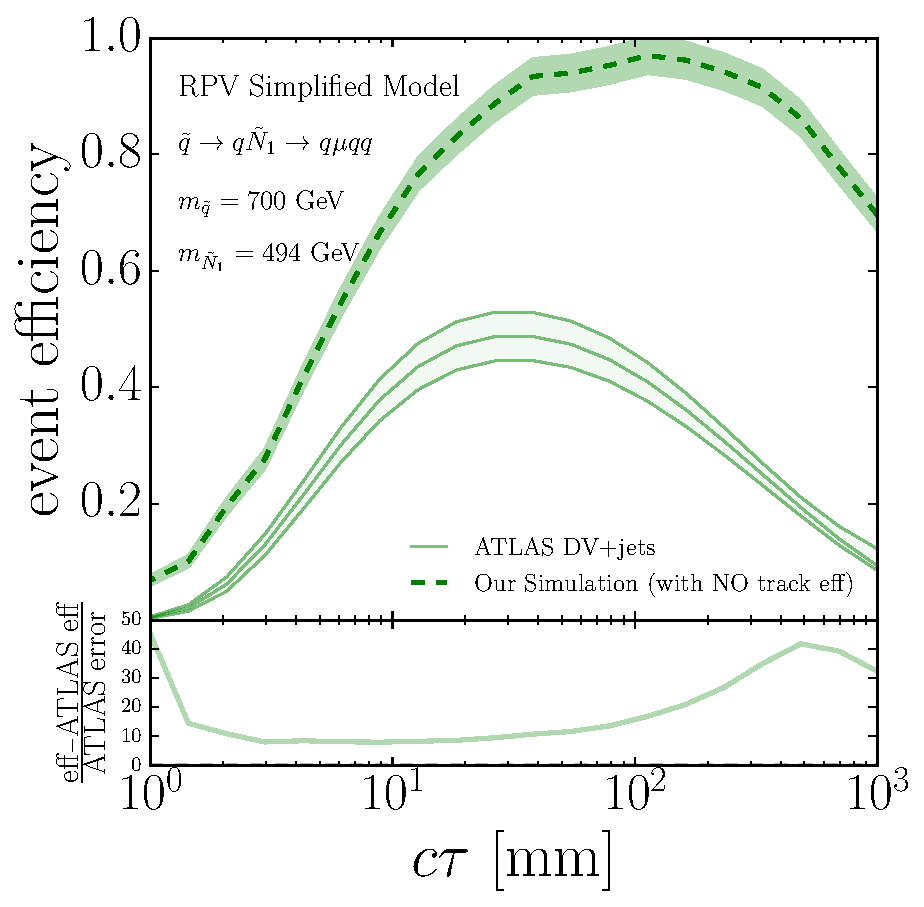
\includegraphics[width=0.45\textwidth,angle=0]{ch5-figures/effVsCtau_RPVValidation_NoTrkEff.pdf}
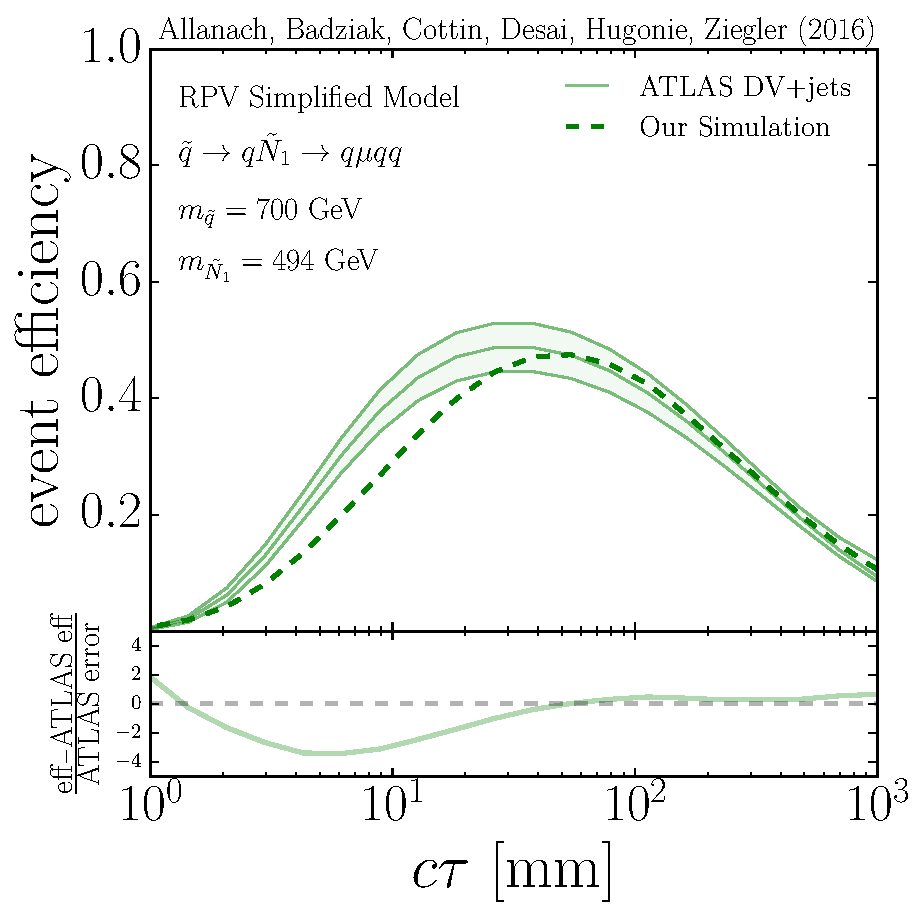
\includegraphics[width=0.45\textwidth,angle=0]{ch5-figures/effVsCtau_RPVValidation.pdf}
\end{center}
\caption{Validation of the DV + jets search for the ATLAS benchmark of a simplified RPV model
  with a 700 GeV squark decaying to a neutralino, $\tilde q \rightarrow q (\tilde N_{1} \rightarrow \mu \bar u d)$ \label{fig:trkeff}. {\bf{Left:}} without any tracking efficiency. {\bf{Right:}} with a tracking efficiency function given by equation~\ref{eqn:trkeff}, taken from Ref~\cite{Allanach:2016pam}.}
\end{figure}

\vskip 0.1in
\noindent {\bf Lessons learned}
\vskip 0.1in

With a larger and more diverse set of signal benchmarks the prospects for reinterpretation are better. For example, the ATLAS analysis examined in~\cite{ATLAS-CONF-2013-092} only showed limits for three signal model benchmark points for which efficiencies were shown, making it challenging to find a benchmark whose kinematics matched the desired signal models for the reinterpretation in Ref.~\cite{Cui:2014twa}. Because the efficiencies and limits were shown for either a high-mass, low-boost LLP \emph{or} a low-mass, high-boost LLP, this made it more challenging to reinterpret the results for other types of kinematics. 

The new parametrized efficiencies presented by ATLAS in~\cite{SUSY-2016-08} are extremely useful. They constitute an optimal efficiency map for recasting these type of analyses, as they can by applied in a straightforward way to truth level quantities. Before this information was public, efficiency tables (for vertex-level efficiency) in terms of $r_\mathrm{DV}$ where only available for few channels and for a single benchmark. It was not clear how to translate it to other channels, and also for parent particles of a different mass. Even more, a functional parametrization for track efficiency was needed (as shown in~\cite{Allanach:2016pam}) to be able to reproduce the experimental results. Finding this kind of parametrization is not easy, as it needs to be validated across different benchmarks. This had the difficulty that fitting only one benchmark did not correctly reproduce the event-level efficiency curve for any of the others.

%\vskip 0.1in
%\noindent {\bf Recommendations} 
%\vskip 0.1in
%
%Parametrized efficiencies as a function of relevant quantities such as: vertex position, its invariant mass and number of charged particles forming it, are extremely useful, as they can allow for reinterpretation of the experimental result for any model predicting displaced vertices. We highly encourage collaborations to keep making such efficiency maps public, and for distinct event topologies, in order to accurately asses the level of model independence.



% Tools
\newcommand{\MG}{\textsc{MadGraph}~5\_aMC@NLO}
\newcommand{\PY}{\textsc{Pythia}~8}
\newcommand{\MA}{\textsc{MadAnalysis}~5}
\newcommand{\MW}{\textsc{MadWidth}}
\newcommand{\MAnorm}{{MadAnalysis}~5}
\newcommand{\FJ}{\textsc{FastJet}}
\newcommand{\DEL}{\textsc{Delphes}}
\newcommand{\ROOT}{\textsc{Root}}

%latin
%\newcommand{\eg}{\textit{e.g.}}
%\newcommand{\ie}{\textit{i.e.}}

% environments
%\def\be{\begin{equation}}
%\def\ee{\end{equation}}
%\def\bsp#1\esp{\begin{split}#1\end{split}}


\section{Handling long-lived particles in \DEL-based detector simulations}
\label{sec:ch5-recastingDelphes}

\subsection{Long-lived particle simulation in \DEL~3.4.1}

The \DEL\ package~\cite{deFavereau:2013fsa} allows for the generic simulation of
the response of a typical detector used in high-energy physics experiments. It
is widely used for simulating the effects of the ATLAS and CMS detectors or the
hypothetical detectors that could be used for the future FCC and CLIC projects.
The architecture of \DEL\ is composed of distinct
and specialized modules that interact with each other. The detector is described
by the user through an input card, where the modules to be used in the
simulation are sequentially enumerated and their input parameters are specified.

The detector simulation relies on a mix of parametric and algorithmic
modules. More precisely, tracking is simulated through efficiency and smearing
functions that are applied to the properties of the electrically-charged stable
particles. The particles are then propagated to the calorimeters and dedicated
modules simulate the energy deposits in the electromagnetic and hadronic
calorimeters. The output of such a step consists in a list of calorimetric towers.
Moreover, \DEL\ includes a particle-flow like
algorithm that combines tracking and calorimetric data in order to
improve the identification of the final-state objects and the resolution on
their reconstructed momenta.

Jet clustering is performed via an internal call to the \FJ\
package~\cite{Cacciari:2011ma}, which takes as input the
list of calorimeter towers or, alternatively, the particle-flow candidates and
outputs jet objects. Lepton and photon isolation is then handled through a
specific isolation module. Finally, \DEL\ takes care of removing the
double-counting of objects that could be simultaneously identified as element of
different collections. The final output is stored in a \ROOT\ file.

In addition, \DEL\ allows for the simulation of pile-up effects by
superimposing minimum-bias events attached to displaced interaction vertices
along the beam direction
to the hard scattering event. Procedures mimicking pile-up
removal can then be configured in the input card. The subtraction of the charged
particles belonging to pile-up vertices is performed at the tracker level.
Neutral particles are removed by applying the jet area
method~\cite{Cacciari:2007fd} supplied within the \FJ\ package. More advanced methods are also available in \DEL, such as the
{\sc Puppi}~\cite{Bertolini:2014bba} or {\sc SoftKiller}~\cite{Cacciari:2014gra}
techniques, and they can easily be added to the input card. The loss of
performance originating from pile-up, in particular relative to the isolation, is
automatically accounted for.

The official \DEL\ package (version 3.4.1) with the default detector cards needs
to be adapted for the proper handling of LLPs.
By default, the decay products of a long-lived particle enter the
simulation as if the corresponding decay would have occurred within the
tracker volume. However, the user has the possibility to define a volume in
which the particle can decay and still be detected outside the tracker volume. This is achieved in
practice by making use of the \verb+RadiusMax+ parameter of the
\verb+ParticlePropagator+ module, that is by default set to the tracker radius
stored in the \verb+Radius+ parameter. When setting the \verb+Radius+ and
\verb+RadiusMax+ parameters to different values, the particles decaying outside
the tracker volume, but inside the `decay volume' of radius \verb+RadiusMax+, are
included in the collection of stable particles stored in the output \ROOT\ file.
They can in this way be used for an offline, more correct, treatment.

Moreover, several modules that are not used in the default ATLAS and CMS cards
could serve for a better simulation of the long-lived particles in \DEL . For
instance, the \verb+TrackSmearing+ module allows the user to smear the track momentum
according to the impact parameter in the transverse plane ({\it i.e.}, the $d_0$
parameter) and in the longitudinal plane ({\it i.e.}, the $d_z$ parameter).

By default, the detector simulation in \DEL\ totally ignores the presence of any
LLP. While this is convenient for neutral particles like a
neutralino which could be considered as invisible from the detector standpoint,
a charged particle leaves tracks in the tracker and would interact with the
calorimeters if its lifetime is large enough.
In this case, if the long-lived particle decays inside the tracker, its
trajectory is properly propagated to the calorimeters and the displaced vertex
is correctly accounted for. However, if the long-lived particle decays outside
the tracker, its decay products are ignored in \DEL, unless the \verb+RadiusMax+
parameter has been specified to be larger than the tracker \verb+Radius+
parameter. In this case the decay products can be found in the
\verb+Delphes/stableParticles+ output collection and
treated with adequate smearing functions and efficiency directly from the \DEL\
output.

Finally, disappearing tracks are simply treated as missing energy in \DEL. Emerging tracks or tracks containing kinks are not treated appropriately, in the sense that the parameterizations required for a proper description of such signatures has not been implemented yet. Also, \DEL\ does not include any trigger simulation, and the latter is in general complex in the case of LLPs.

\subsection{Displaced tracks with the \MA\ tune of \DEL}

The so-called \DEL-LLP package can be installed from the version v1.6 of
\MA~\cite{Conte:2012fm,Conte:2014zja} and contains improvements of \DEL\
specific to LLPs. It leads to new possibilities for phenomenological investigations of long-lived
particles and the recasting of related LHC analyses~\footnote{More information is
available at the following website:\\ \noindent \url{https://madanalysis.irmp.ucl.ac.be/wiki/MA5LongLivedParticle}}.

This new package was designed to handle neutral LLPs that decay
into leptons within the tracker volume. Realistic efficiencies are applied to
the displaced tracks and several parameters specific to this kind of analysis
have been made available within \MA. An extension to the case of neutral
LLPs decaying into muons outside the tracker volume can be easily
implemented, the muons being thus reconstructed only through their hits in the
muon chambers. The simulation of the displaced leptons is performed through efficiencies and resolution functions to be specified by the user. Furthermore, another
extension allowing the user to handle long-lived charged particles that decay into
leptons could be implemented.

The \DEL-LLP package contains a new module called \verb+MA5EfficiencyD0+ that
allows for the definition of a track reconstruction efficiency parameterized as a function of the $|d_0|$ and $d_z$ parameters (named \verb+d0+ and \verb+dz+ in the \DEL\ input
card). The default efficiency function, specified via a \verb+DelphesFormula+ is taken from the
8~TeV tracking performance of CMS~\cite{Khachatryan:2014mea}~\footnote{\url{https://twiki.cern.ch/twiki/bin/view/CMSPublic/DisplacedSusyParametrisationStudyForUser}},\\
\begin{verbatim}
 set EfficiencyFormula {
   (d0<=20) * (-5.06107e-7 * d0**6 + 0.0000272756 * d0**5 - 0.00049321 * d0**4
      + 0.00287189 * d0**3 + 0.00522007 * d0**2 - 0.0917957 * d0 +  0.924921) +
   (d0> 20) * (0.00)
 }
\end{verbatim}
In addition, the data-format of \DEL\ has been extended so that the \verb+Muon+ and
\verb+Electron+ classes now include the transverse ($|d_0|$) and longitudinal ($d_z$) impact parameters relative to the closest approach point (encoded
in the \verb+d0+ and \verb+dz+ variables), the coordinates of the closest
approach point $(x_d, y_d, z_d)$ (encoded in the \verb+xd+, \verb+yd+ and
\verb+zd+ variables) and the four-vector of the vertex from which the lepton is
originating from $(t_p, x_p, y_p, z_p)$ (encoded within the \verb+tp+,
\verb+xp+, \verb+yp+ and \verb+zp+ variables), the latter quantity being
evaluated from Monte Carlo information.

%\renewcommand{\arraystretch}{1.2}
%\setlength{\tabcolsep}{12pt}
\begin{table}[t]
\begin{center}
  \begin{tabular}{l || l | c  c | c }
    Region & $c\tau_{\tilde t}$ [cm] & MA5 & CMS& Difference [\%] \\ \hline\hline
%    \multirow{4}{*}{\bf SR-1}& 0.1 & 3.89   & 3.8  & 2\\
    \multirow{4}{*}{\bf SR-1}& 0.1 & 3.89   & 3.8  & 2\\
                             & 1   & 4.44   & 5.2  & 15\\
                             & 10  & 0.697  & 0.8  & 15\\
                             & 100 & 0.0610 & 0.009& $> 100\%$\\ \hline
    \multirow{4}{*}{\bf SR-2}& 0.1 & 0.924  & 0.94 & 2\\
                             & 1   & 3.87   & 4.1  & 5\\
                             & 10  & 0.854  & 1.0  & 15\\
                             & 100 & 0.0662 & 0.03 & $\sim 100\%$\\ \hline
    \multirow{4}{*}{\bf SR-3}& 0.1 & 0.139  & 0.16 & 15\\
                             & 1   & 6.19   & 7.0  & 10\\
                             & 10  & 4.45   & 5.8  & 25\\
                             & 100 & 0.497  & 0.27 & 85\\
  \end{tabular}
  \caption{Number of events populating the three signal regions (SR-1, SR-2 and SR-3) of Ref.~\cite{CMS-PAS-EXO-16-022}
   for different stop decay lengths ($c\tau_{\tilde t}$).
    We compare the CMS and \MA~(MA5) results in the second
    and third column of the table, respectively, and the difference taken relatively to CMS is
    shown in the last column.}
  \label{tab:cms_exo}
\end{center}
\end{table}
\renewcommand{\arraystretch}{1}


Consequently, the data-format of \MA\ has been extended, so that the \verb+Muon+ and
\verb+Electron+ classes now contains the \verb+d0()+ and \verb+dz()+ methods allowing to
access the value of the $|d_0|$ and $d_z$ parameters, the \verb+closestPoint()+
method that returns the coordinates of the closest approach point (through the
\verb+X()+, \verb+Y()+ and \verb+Z()+ daughter methods) and the
\verb+vertexProd()+ method that returns coordinates of the displaced vertex from
which the lepton originates from (through the \verb+X()+, \verb+Y()+ and
\verb+Z()+ daughter methods). An analysis example \cite{MA5:longlivedleptons} can be found in the public analysis database of \MA~\footnote{ \url{http://madanalysis.irmp.ucl.ac.be/wiki/PublicAnalysisDatabase}},
where information about the re-implementation in \MA\ of Ref.~\cite{CMS-PAS-EXO-16-022}  
analysis of 2.6~fb$^{-1}$ of 13~TeV LHC data is available. This is a search for long-lived particles decaying into electrons and muons, where signal
events are selected by requiring the presence of either an electron or a muon
whose transverse impact parameter lies between 200~$\mu$m and 10~cm. For a given
benchmark signal where a pair of long-lived stops is produced through usual QCD
interactions and where each stop further decays into a displaced $b$-jet and a
displaced lepton. In Table~\ref{tab:cms_exo}, we present the number of events
surviving the selection of the three different signal regions of the CMS analysis.
Our event generation has been preformed with {\sc Pythia} 8~\cite{Sjostrand:2007gs}
and for the benchmark
scenario SPS 1a.
We observe that a good agreement is obtained, except in the case of a long stop
lifetimes, $c\tau \gtrsim 1$~m. 
This is however the region in which no public information on
the CMS reconstruction efficiencies is available.

The \MA\ tune of \DEL\ has neither been designed for disappearing
(or appearing) tracks nor for track kinks. Concerning the disappearing (or appearing)
tracks, the only missing experimental ingredients are the track reconstruction efficiency
and resolution as a function of the number of missing hits in the (inner) outer
layers of the tracker. There is to this date no public material on the tracking
performance description related to track kinks.

\subsection{What about other LLP signatures?}

In this section, we briefly discuss how \DEL\ could be improved for a better
handling of LLP signatures.

\subsubsection{Displaced jets}
\label{sec:dispjets}

Displaced jets are jets that are reconstructed either from stand-alone calorimeter
information, or from the particle-flow input with a minimum requirement on the
multiplicity of tracks with high transverse displacement (see
Ref.~\cite{CMS:2014wda}). Conceptually, such jets can be handled in \DEL\
provided that the displaced tracks are properly parametrized. As described
above, a module designed to smear the full set of track properties, including
their transverse and longitudinal displacement, exists ({\it i.e.}, the
\verb+TrackSmearing+ module). In addition, efficiencies based on displacement
parameters have already been implemented in \MA\ (see above) and a module that
performs the matching of an existing jet collection with a track collection
based on track displacements is very similar to the already existing
\verb+TrackCountingBTagging+ module. Minor modifications to this module are
hence needed to be able to select tracks based on an absolute displacement
instead of the impact parameter significance. Finally, in order to be able to
perform a displaced jet selection, one would need a (not-yet existing) module
that performs jet clustering on the basis of the secondary vertices based and
the displaced tracks matched with these jets. Alternatively, a module that
includes a vertex reconstruction efficiency and a module including a vertex
position smearing could be implemented.


\subsubsection{Displaced vertices}

The missing modules described in Section~\ref{sec:dispjets} could perfectly
serve the purpose of a displaced vertex analysis. Provided that tracking
efficiencies and resolutions are available as a function of the full set of
tracking parameters ($d_0$, $d_z$, $p_T$, $\phi$, and $\theta$ ) and,
eventually, of the Monte Carlo truth vertex position, a simple vertexing
algorithm can be implemented in \DEL.

\subsubsection{Discussion: \DEL\ versus a specific parametric simulation}

In a fully parametric simulation of the detector, the detector effects are encoded in
terms of efficiencies and resolution functions. Such a simulation is
typically very fast, but is likely to suffer from a lack of accuracy in the
modeling of complex observables such as jet properties and missing energy. The
\DEL\ simulation is an admixture of such a parametric simulation, and of an
algorithmic one. This is slower, but has the clear advantage of correctly
treating in particular the reconstruction of the jets and the missing energy.

In order to be able to answer whether \DEL\ should be used in place of a fully
parametric simulation in recasting  LLP analyses,
further studies are needed. In the meantime, the following guidelines could be
used. If the signal selection is based only on displaced tracks, a simple
parametric simulation should in principle be sufficient. This simulation could encapsulate the
track reconstruction efficiency and resolution, including pile-up effects. \DEL\
could then optionally be used to mix the resulting ``reconstructed" tracks with the additional tracks originating from the pile-up vertices.
On the other hand, if the analysis under consideration additionally uses
calorimetric information ({\it i.e}, jets or missing energy), \DEL\ should be
preferred to a fully parametric framework. However, a precise
quantification of these effects cannot be assessed without detailed comparative
studies between the two approaches. Finally, it should be pointed out that
neither of these techniques can be used to correctly simulate the instrumental background,
which is challenging to simulate and is discussed in Chapter \ref{sec:backgrounds}.



\section{Recasting Inside the Experimental Collaborations}
\label{sec:ch5-recastingInsideExp}

Reinterpretations performed within the experiments themselves present unique advantages and disadvantages. They allow for thorough and consistent treatment of detector effects and geometry, object reconstruction, and systematic uncertainties in a way which is impossible through external recasting. Groups can share resources and easily communicate all necessary details. On the other hand, they are of course limited to the model(s) chosen for reinterpretation. In the ideal situation, reinterpretation(s) which provide meaningful results can be performed with minimal overhead to a given analysis.

As the LHC enters an era of deccelerating luminosity growth and following  trends towards more sophistication in analysis techniques, the LHC analyses become harder to re-implement with sufficient accuracy outside of the experiments compared to cut-based analyses. Analyses increasingly utilize machine-learning algorithms that transform a large number of event-level and particle-level observables into higher-level discriminants, which are not easily characterized by low-dimensional efficiency tables and may require inputs that third-party detector simulations are not able to reproduce. In particular non-prompt searches may depend on non-traditional reconstruction objects and details of the detector simulation and geometry in ways that require a more detailed simulation than is achievable by, \emph{e.g.}, third-party simulators. Hence, experiments are investigating approaches that enable internal re-interpretation using the full set of available information.

Full-fidelity reinterpretations are  especially relevant for long-lived particles, since the signal simulation may depend more heavily on details not well captured by third-party simulation tools. For example, for sufficiently high lifetime, the decays must be handled by a full detector simulation such as GEANT (or some complex interaction between GEANT and MC packages such as Pythia). Such decays are not well-covered by tools like Delphes as the response of such in-detector decays may require access to a more detailed geometry description.

\subsection{The RECAST Framework}

The RECAST Framework~\cite{Cranmer2011} is a developing platform for experiments as well as  researchers external to the collaborations who wish to reinterpret LHC analyses. RECAST enables cloud-based analysis execution and common presentation of reinterpretation results. The framework consists of two components:

\paragraph{The RECAST front-end} This is a web-based service in which reinterpretation of analyses can be suggested by interested authors that provide necessary inputs such as UFO model files \cite{Degrande:2011ua}, process and parameter card templates, or suggested scan grids. Responses to such requests, possibly by more than one analysis implementation, can then be uploaded. Such a web service, interfaced with services such as HepData, may then serve as a resource for the LHC community to organize and share reinterpretation results obtained by the various analysis implementations.

\paragraph{The RECAST back-end} An important objective of the framework is to enable a full-fidelity reinterpretation of an LHC analysis using the original analysis code developed within the experiment that can be approved by the collaboration and be placed on an equal footing with the original publication. In contrast to third-party recasting tools, in which multiple analyses are implemented using a single, common framework that is  executed on a single computing element, such an exact analysis re-execution often necessitates a distributed data analysis using a number of different frameworks in use within the experiments. Therefore, RECAST has developed a flexible graph-based, analysis description and execution backend[cite ACAT 2017] that enables a faithful re-execution of nearly arbitrary analysis code on cloud platforms such as those offered by CERN\footnote{Thanks to this flexibility, the popular third-party recasting tools can  be easily integrated into this back-end as well, with current integrations being available for CheckMate and Rivet.}. The back-end provides experiments with an access-controlled interface to view reinterpretation requests, retrieve the necessary analysis description from repositories such as the CERN Analysis Preservation Portal (CAP)~\cite{CAP},  execute the analysis on datasets for the new model and -- if approved -- upload the results to the public front-end. Figure~\ref{fig:recast-cc} shows a screenshot of the current prototype user interface, giving collaboration members an overview over requested points as well as controls to steer processing and submission.

\begin{figure}[t]
\begin{center}
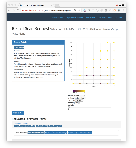
\includegraphics[width=0.5\textwidth,angle=0]{ch5-figures/requestview.pdf}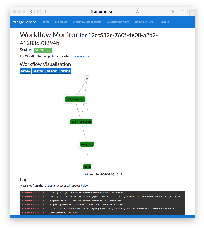
\includegraphics[width=0.5\textwidth,angle=0]{ch5-figures/monitor.pdf}

\end{center}
\caption{
Left: Web-based interface for RECAST backend for experiment that presents the requested parameter points and color-coded results,
Right: An experiment-internal reinterpretation executing on the distributed infrastructure built by CAP and RECAST.}
\label{fig:recast-cc}
\end{figure}

These services are being developed in close collaboration with the CERN Analysis Preservation project, which is a common project supported by the four major LHC experiments. While this integration work is on-going, the computing backend for RECAST has been successfully used for a number of Run-1 and Run-2 reinterpretations published by the ATLAS Experiment.


\subsection{Analysis Preservation as a driver for re-interpretation}

Within the LHC experiments, the ability to re-interpret analyses is, perhaps unintuitively, mostly limited by the internal availability of the analysis routines to the wider collaboration as opposed to, \emph{e.g.}, availability of computing resource constraints. The large number of measurements and searches, the heterogeneity and complexity of the analysis software, as well the size of the collaboration all lead to a situation in which  only a small number of analyzers of the original analysis team are often-times able to execute any given analysis. Furthermore, due to the collaborative development model, analyzers  are typically responsible for only a subset of the analysis, which results in knowledge fragmentation. Therefore, both ATLAS and CMS are now designing an interface to store analysis-relevant information (the CERN Analysis Preservation Portal, CAP~\cite{CAP}) to mitigate this problem. In the context of RECAST, the software and analysis-workflow preservation aspects of this effort are most relevant. The former is mainly implemented through archiving of source-code repositories and the archival Linux Containers, which now enjoy wide-spread industry support, while internal structure of the analysis workflow is archived in CAP in the form of declarative workflow specifications such as yadage~\cite{Cranmer:2017frf}, which has been developed for RECAST, and the Common Workflow Language (CWL)~\cite{CWL}. It is planned that CAP and RECAST will utilize a common computing back0end in order to re-execute the analyses that have been preserved in the portal. As the preservation is enabled by recent technological advances and the process of archival is increasingly streamlined, it is expected that a higher number of  experiment-internal analysis codes will be available for RECAST.



\subsection{RECAST Examples}

\paragraph{ATLAS-internal Analysis Examples and Results :}

A number of re-interpretation publications have been supported by the backend underpinning RECAST. After Run 1, ATLAS has conducted a thorough re-interpretation of the SUSY landscape in the context of the phenomenological pMSSM~\cite{Aad:2015baa}, a study involving 20 SUSY analyses and 50,000 fully simulated pMSSM parameter points. While at that time, most analyses had to be re-interpreted manually, the 2L electroweak analysis~\cite{Aad:2014vma} included in that paper served as a prototype analysis and provided results using the highly automated RECAST back-ends.

The analysis was than later re-used with minimal additional effort in two additional publications that focused on more domain-specific SUSY realizations:~a five-dimensional dark-matter reinterpretation of electroweak seaches~\cite{Aaboud:2016wna}, as well as a reinterpretations in the context of general gauge-mediated models~\cite{ATLAS-CONF-2016-033}.

\begin{figure}[t]
\begin{center}
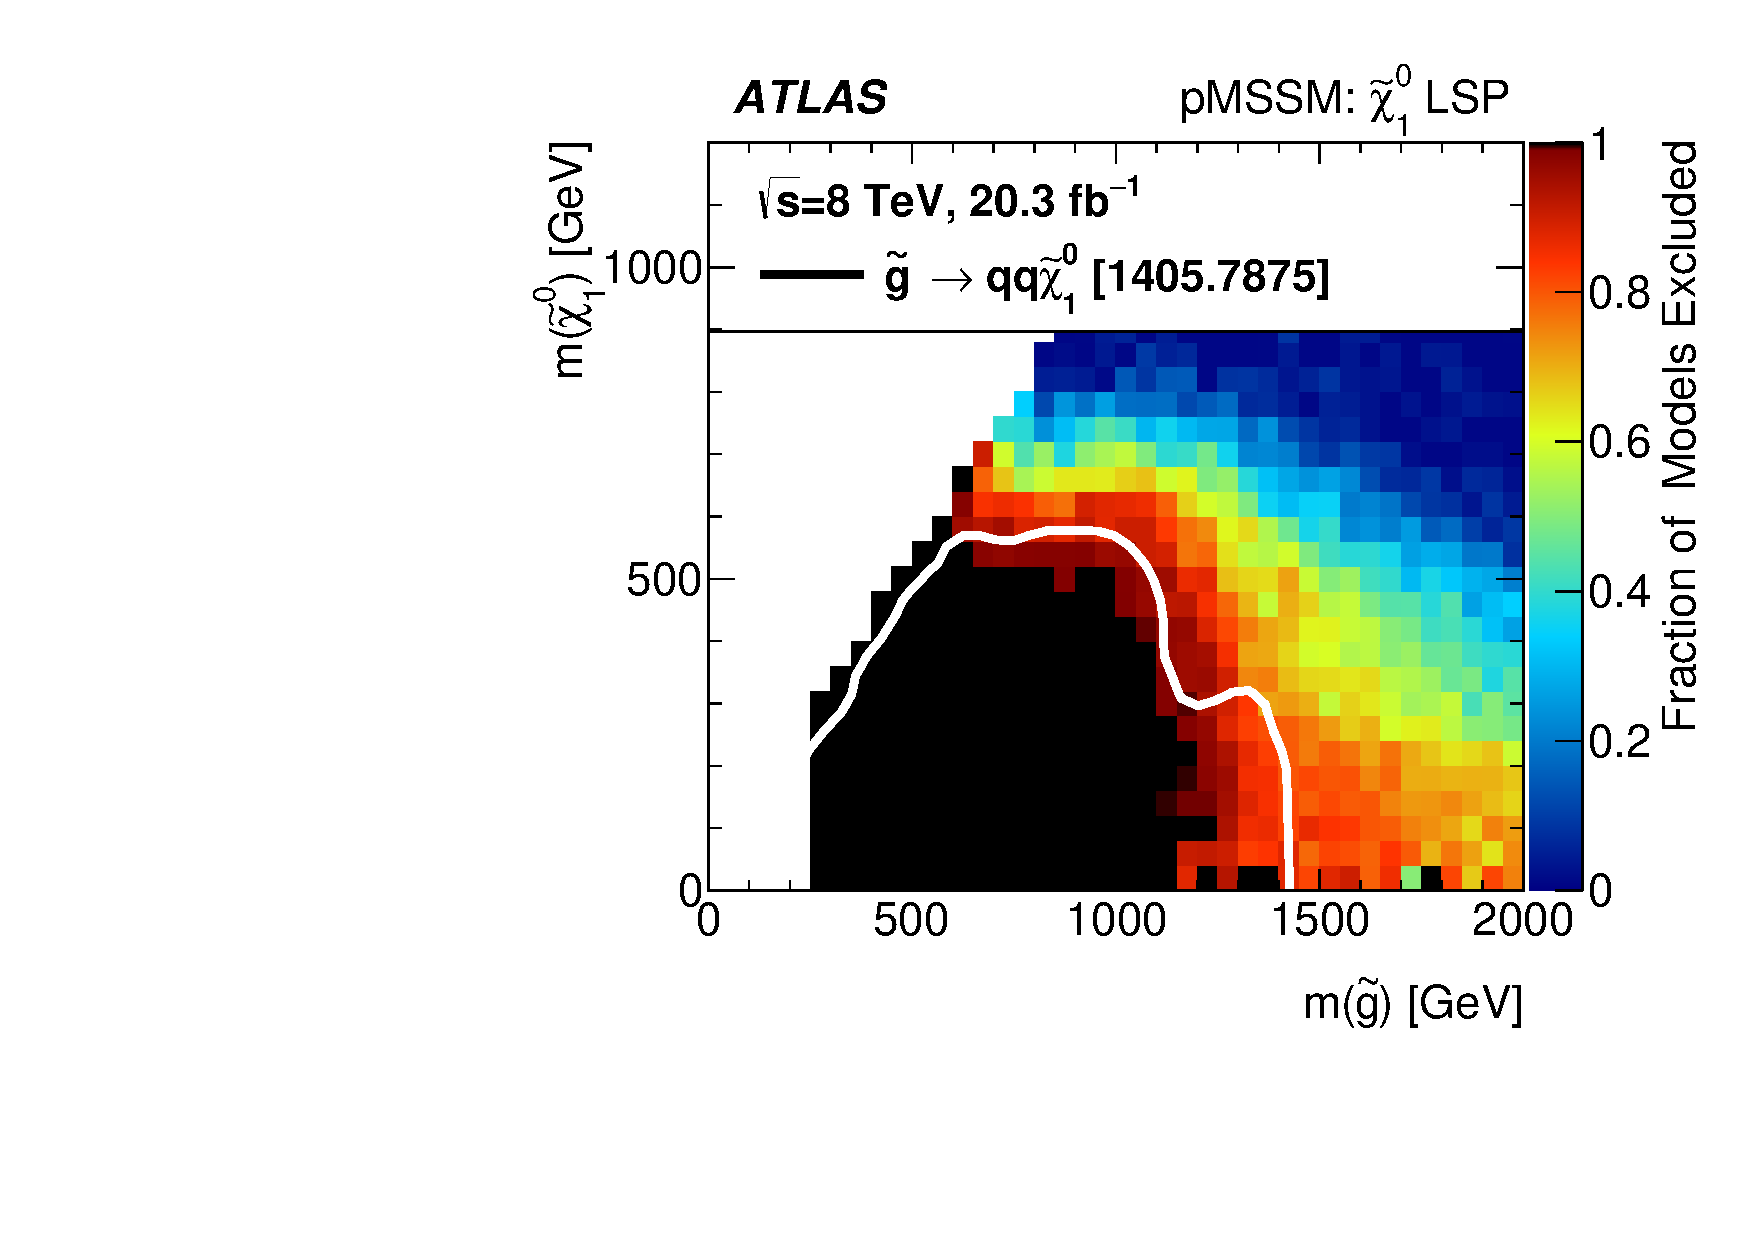
\includegraphics[width=0.48\textwidth,angle=0]{ch5-figures/pMSSM.pdf}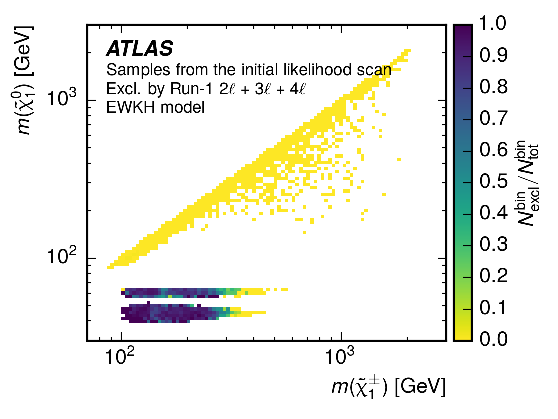
\includegraphics[width=0.52\textwidth,angle=0]{ch5-figures/DM.pdf}

\end{center}
\caption{
Left: pMSSM exclusion in the gluino-neutralino mass-plane. Results partially provided by RECAST.
Right: Follow-up dark-matter re-interpretation. Exclusions presented in chargino-neutralino mass-plane.
}
\label{fig:recast-cc}
\end{figure}


% Currently, a number of additional Run-2 analyses are in the process of being re-interpreted with results expected to appear soon.

Recently ATLAS has reinterpreted 10 analyses~\cite{ATLAS:2018yey} in terms of models of supersymmetry with non-vanishing baryon-number violating coupling strength $\lambda''$ partly through the use of the new analysis preservation infrastructure. In such models the lighest neutralino it unstable with a decay length of

\begin{equation}
  L(cm) = \frac{0.9\beta\gamma}{{\lambda''}^2} \left(\frac{m(\bar{q})}{100\mathrm{GeV}}\right)^4\left(\frac{1\mathrm{GeV}}{m(\tilde{\chi}_1^0)}\right)^5.
\end{equation}

This reinterpretation required a joint re-execution of a mix of analyses originally designed for R-parity-conserving and R-parity-violating models and special systematics have been added into the statistical analyses to account for the detector response and flavor-tagging rate of displaced-ets. Results were presented in a two-dimensional parameter space of gluino mass and neutralino lifetime (or analogously the $\lambda''$ coupling) as shown in Fig.~\ref{fig:rpvrpc}. Such reinterpretations are difficult to perform outside of the experiments, as the publicly available information lack details of the detector and analayses.

\begin{figure}[h]
\begin{center}
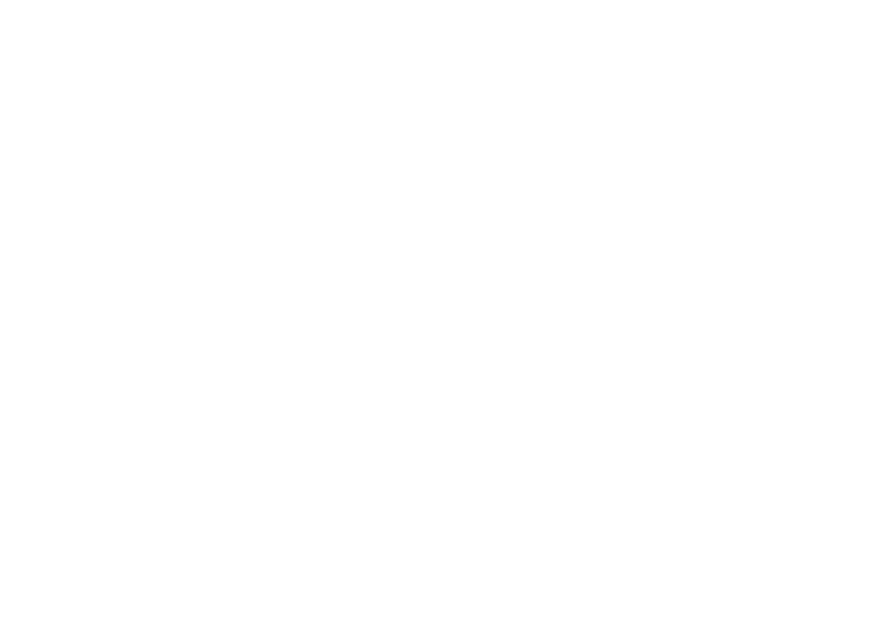
\includegraphics[width=0.85\textwidth,angle=0]{ch5-figures/fig_04.pdf}
\end{center}
\caption{Exclusion limits as a function of $\lambda''_{323}$ and $m({\tilde{g}})$. Expected limits are shown with dashed lines, and observed as solid. Taken from Ref.~\cite{ATLAS:2018yey}.}
\label{fig:rpvrpc}
\end{figure}



\paragraph{Third-Party Tool Integration }

Both the CheckMate~\cite{Drees:2013wra,Dercks:2016npn} and the Rivet~\cite{Buckley:2010ar} analysis catalogues have been implemented in the analysis-execution framework. Both are configured to analyze events that are provided in the HepMC format
\cite{Dobbs:2001ck}. Due to the modular approach of the analysis back-end, a number of MC generation workflows, such as Herwig~\cite{Marchesini:1991ch}, SHERPA~\cite{Gleisberg:2008ta} or MadGraph~\cite{Alwall:2011uj}, can be used depending on their ability to correctly model the desired signal.

For analyses where multiple implementation exists, \emph{e.g.,} from multiple third-party tools such as Rivet BSM, CheckMate or MadAnalysis~\cite{Conte:2014zja,Dumont:2014tja} as well as from multiple experiment-internal configurations (fast Simulation, full simulation), RECAST will allow the community to compare and contrast reinterpretation results.

\subsection{Outlook}

Thanks to industry-backed technological advances, a realistic technical solution to the Analysis Preservation problem for the LHC experiments and the original RECAST proposal has come into view. The initial use of such infrastructure for the reinterpretation for prompt SUSY searches is generalized easily for long-lived particle searches as the tools used for  signal simulation, analysis preservation, and execution do not make simplifying assumptions on the nature of the BSM signal or analysis structure.  As such, RECAST may cover reinterpretation use-cases, where either third-party reinterpretations are impossible due to missing public information or limitations of third-party tools or accurate, experiment-approved results are desired.
 

\section{Reinterpretation with Prompt Analysis}\label{sec:ch5-recastingPrompt}

% Depending on the lifetime, a part of the LLP decays will always happen
% outside the detector, leading to a \MET signature if the LLP is
% electrically and color neutral. Likewise, some part of the LLP decays will always appear
% ``promptly". Prompt searches with and without \MET can therefore provide
% additional, corroborating constraints on models with LLPs. Therefore, it is
% important to understand the sensitivity of prompt searches to displaced objects.

% Reinterpreting prompt searches in the context of LLPs is, however,
% quite nontrivial, because not all prompt searches make explicit
% requirements on the primary vertex. Moreover, it is not documented how
% reconstruction efficiencies drop as a function of small displacement.
% Thus, the reinterpretation of prompt searches in the context of LLPs is
% currently best done within the collaborations themselves.

Since the decay time probability of an unstable particle follows an
exponential decay law, depending on the mean lifetime a part of the LLP
decays will happen outside the detector, leading to a \MET signature if the LLP is
electrically and color neutral. Likewise, some part of the LLP decays
can appear ``promptly". Prompt searches with and without \MET can
therefore provide additional, corroborating constraints on models with
LLPs, especially for short lifetimes. Therefore, it is important to
understand the sensitivity of prompt searches to displaced objects.

Reinterpreting prompt searches in the context of LLPs is, however,
quite nontrivial, because {\it a)} prompt searches may or may not make
explicit requirements on the primary vertex and {\it b)} it is
currently not documented how reconstruction efficiencies drop as a
function of small displacement. Thus, the reinterpretation of prompt
searches in the context of LLPs is currently best done within the
collaborations themselves.


An example of such an experiment-internal reinterpretation can be found in a CMS
search for an RPV SUSY model where pair-production of stops each proceed through
an R-parity violating decay to a $b$ quark and a lepton. A dedicated long-lived
search for this model exists in the $e\mu$ channel~\cite{CMS-PAS-EXO-16-022}.
This search includes selection criteria which require the transverse impact
parameter to the interaction point be greater than 10 $\mu$m. This maximizes
sensitivity to the long-lived model and greatly reduces standard model
backgrounds. It also necessarily highly reduces the sensitivity of the search at
low stop lifetime. The exclusion curve in the stop lifetime ($c\tau$) vs. top
squark mass is shown in the left frame of Figure~\ref{fig:exo-16}.

A reinterpretation was performed by a search for pair-production of second
generation leptoquarks (LQs)~\cite{CMS-PAS-EXO-16-007,Sirunyan:2018ryt}. In this model, massive
leptoquarks are pair-produced.  Each of these bosons then decay to a muon and
$c$ quark, leading to a final state with two muons and two jets from $c$ quarks.
In the prompt limit of the RPV SUSY model with a final state of two muons and
two jets from $b$ quarks, the kinematics of the LQs is nearly identical. In the
LQ search, no selection is made on jet flavor. The LQ search uses final
selections which are optimized to the event kinematics for each LQ mass
hypothesis, but the search in general strives to remain as model-independent as
possible. In this case, the reinterpretation was simply performed using the
original LQ analysis, and replacing the signal samples with the long-lived RPV
samples, only taking into account the reduced branching fraction to the two
muons, two jets final state. The expected and observed exclusion curves of the
reinterpretation are shown in the right frame of Fig.~\ref{fig:exo-16}.

The reinterpretation gives large improvement for lifetimes $\leq1$mm, and as
expected, contributes little in the large lifetime limit. This type of
reinterpretation is valuable not only because it extends coverage of a given
model, but also because it helps guide the analysts performing the dedicated
search to focus their efforts in areas which are truly uncovered.

Reinterpretations like this one, which provide meaningful results without
placing a large burden on analysis teams, should be highly encouraged. Other reinterpretations along
these lines can be found in Refs.~\cite{ATLAS-CONF-2014-037,Sirunyan:2018vjp,Aaboud:2018iil}. Another relatively simple
reinterpretation is Ref.~\cite{ATLAS-CONF-2018-003}, although in this case, it
should be noted that the original analysis was modified in a simple way, that is,
the reliance on tracking information to identify jets and suppress non-collision background was
removed, in order to be sensitive to long-lived gluinos.

\begin{figure}[t]
\begin{center}
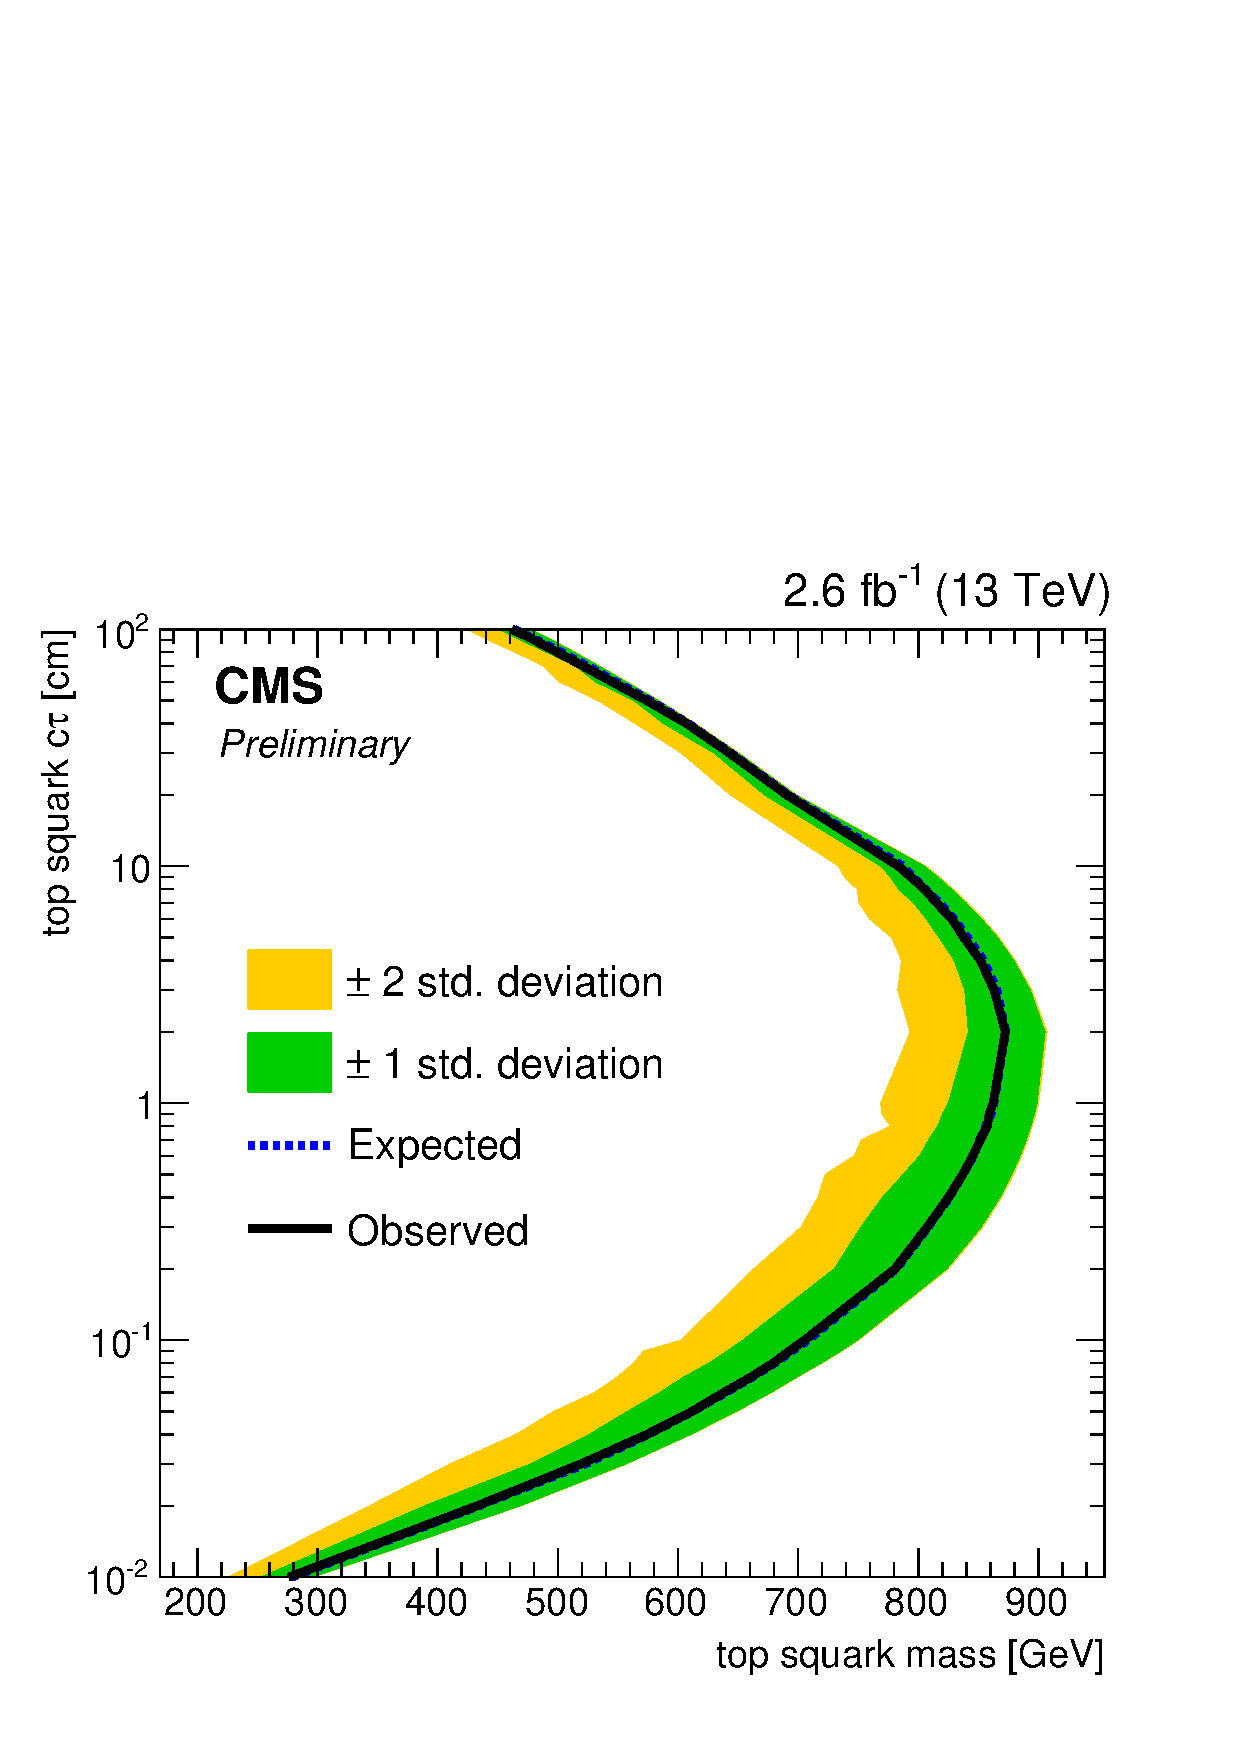
\includegraphics[width=0.45\textwidth,angle=0]{ch5-figures/CMS-PAS-EXO-16-022_Figure_004.pdf}
% 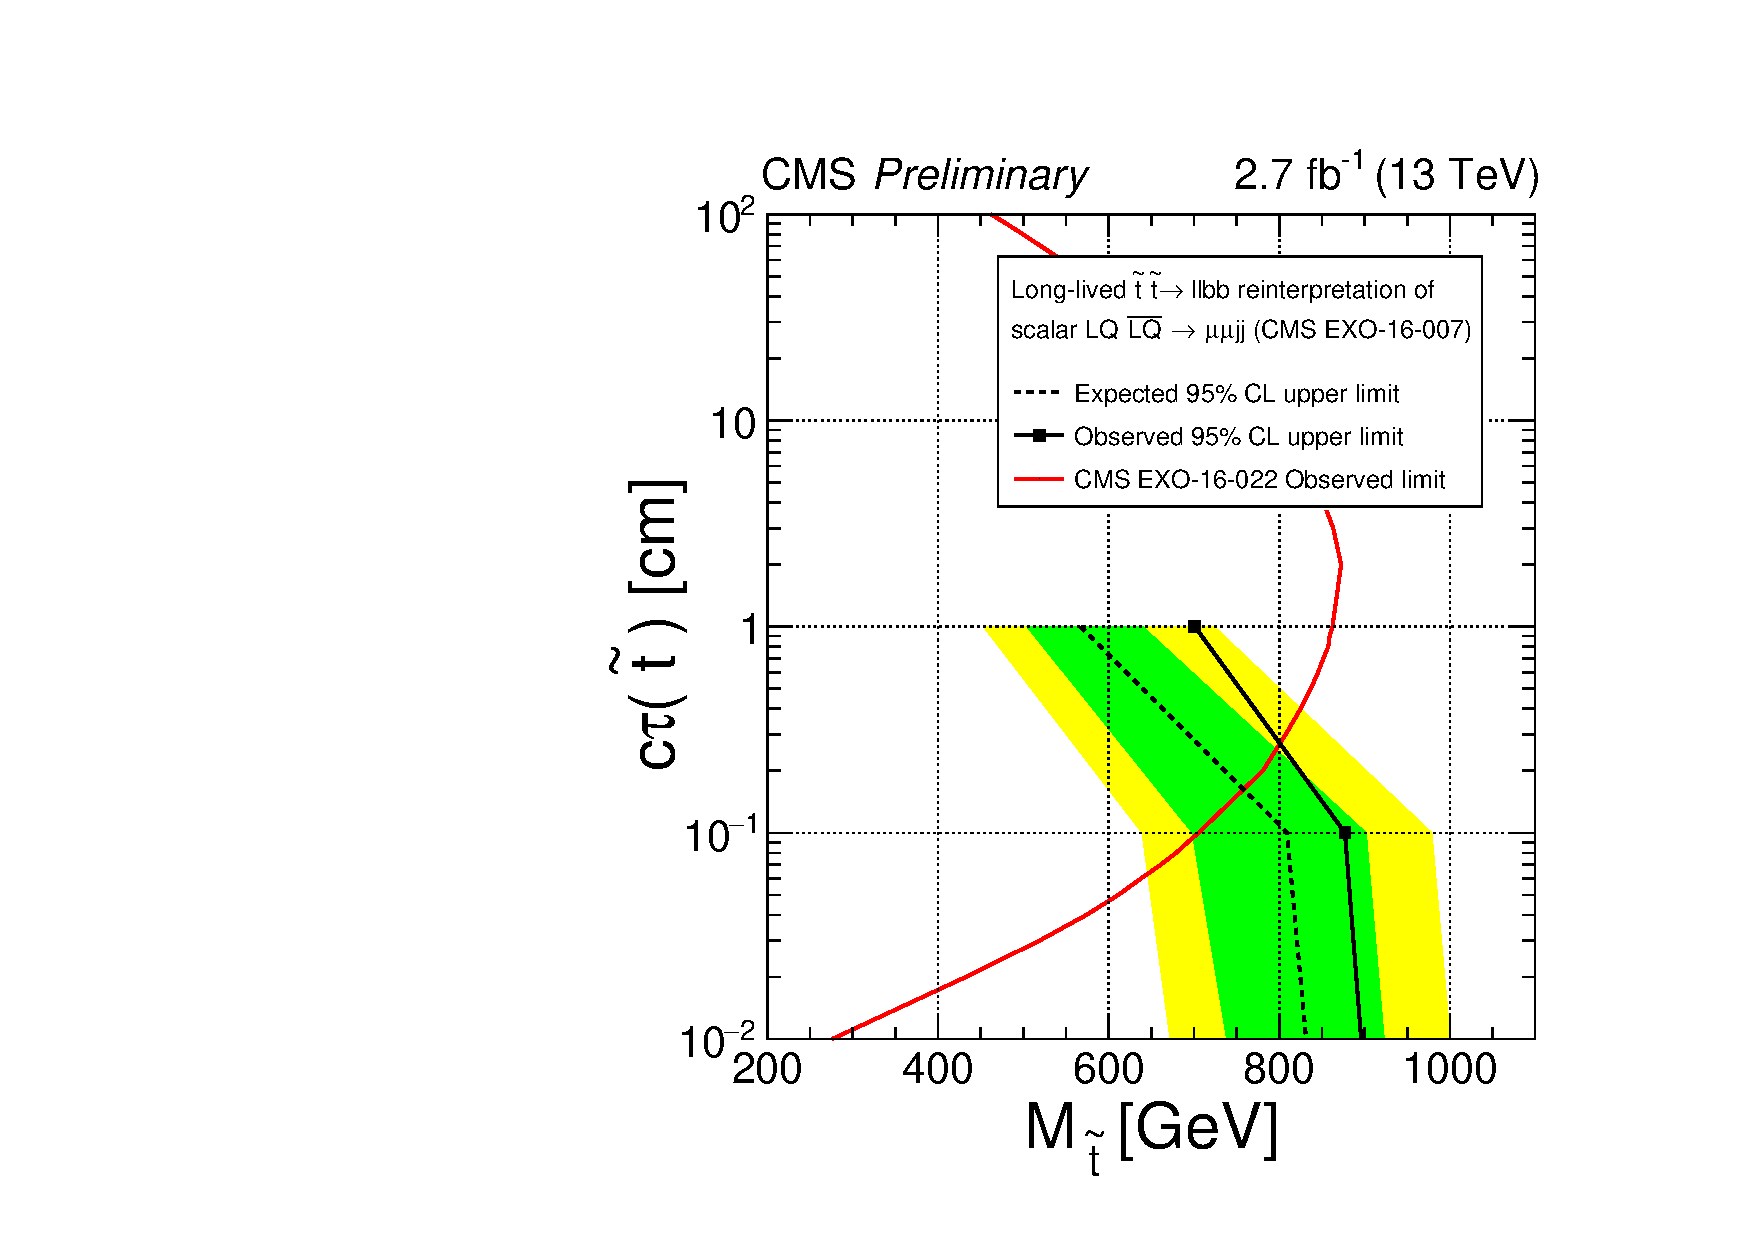
\includegraphics[width=0.5\textwidth,angle=0]{ch5-figures/CMS-PAS-EXO-16-007_Figure-aux_001.pdf}
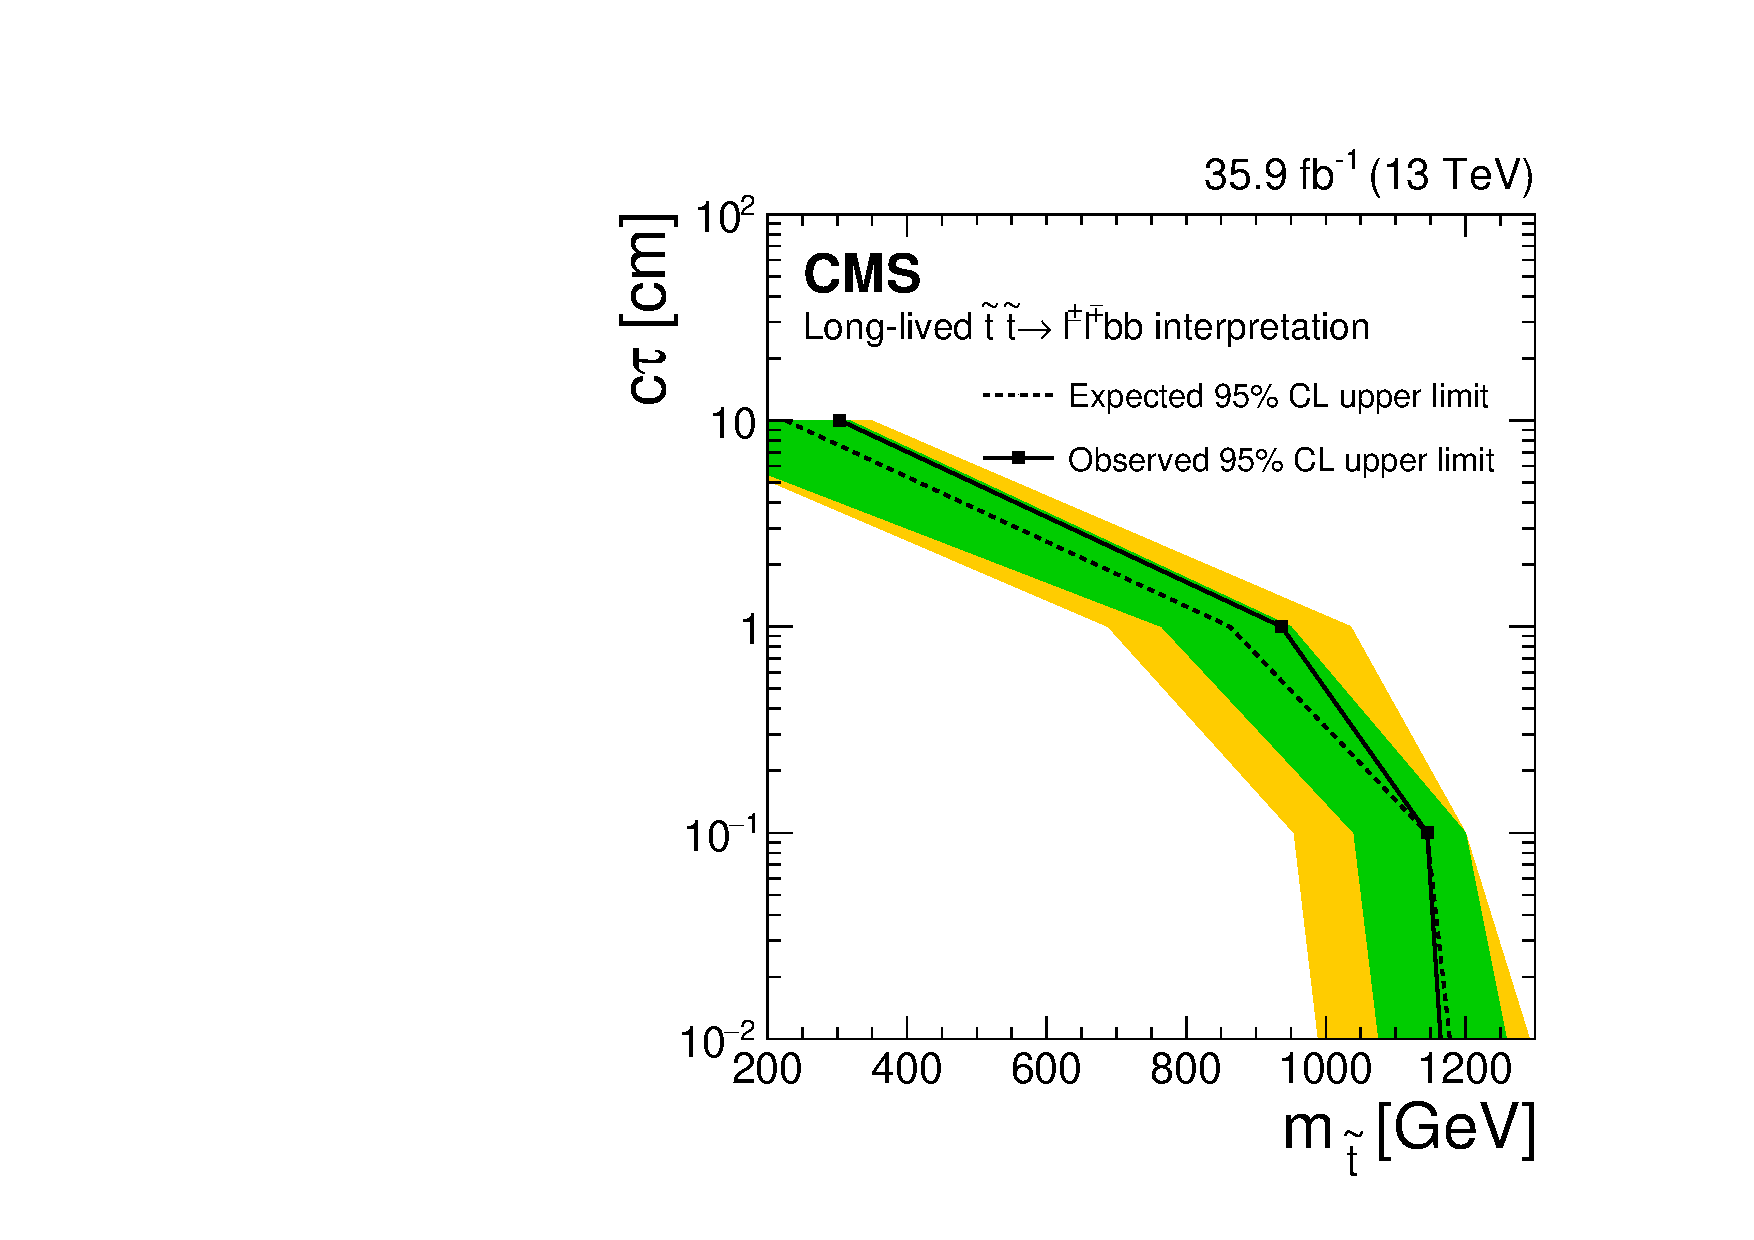
\includegraphics[width=0.45\textwidth,angle=0]{ch5-figures/CMS-EXO-17-003_Figure_010.pdf}
\end{center}
\caption{{\bf Left:} Expected and observed $95\%$ confidence level limits in the $c\tau$-M$_{\tilde{t}}$ plane from the displaced lepton search~\cite{CMS-PAS-EXO-16-022} for pair-production of long-lived stops decaying to $b$ quarks and leptons. {\bf Right:}
Exclusion on pair-production of long-lived stops decaying to $b$ quarks and leptons in the $c\tau$-M$_{\tilde{t}}$ plane, from the prompt reinterpretation of the second generation LQ search~\cite{Sirunyan:2018ryt}.} %Exclusion in the $c\tau$-M$_{\tilde{t}}$ plane from the prompt reinterpretation of pair-production of long-lived stops decaying to $b$ quarks and leptons~\cite{Sirunyan:2018ryt}. }%Exclusion from the dedicated long-lived search in Ref.~\cite{CMS-PAS-EXO-16-022} is overlaid with a solid red line~\cite{CMS-EXO-16-007url}.}
\label{fig:exo-16}
\end{figure}





\section{Our Proposals for the Presentation of Results}
\label{sec:ch5-rec_summary}

Here we summarize the recommendations for the presentation of long-lived
particles search results. These recommendations follow from the detailed
examples presented in Sections~\ref{sec:ch5-smsReinterpretations}
and~\ref{sec:ch5-recastExamples}.

Our primary recommendation is that the experiments provide as detailed
information as possible to make a general recasting possible.
We therefore encourage the experiments to:
\begin{description*}
  \item[A.1.] Provide LLP reconstruction and selection efficiencies at the signature or object level. Although the parametrization of efficiencies is strongly analysis dependent, it is of advantage if they are given as a function of model-independent variables (such as functions of displaced vertex $d_0$, $p_T$, $\eta$, etc.), so
  they do not rely on a specific LLP decay or production mode;
  \item[A.2.] Present results for at least two distinct benchmark
  models, with different event topologies, since it greatly helps to validate the recasting. For clarity, the input cards for the benchmark points should also be provided;
  \item[A.3.] Present cut-flow tables, for both the signal
    benchmarks and the background, since these are  very useful for
    validating the recasting;
  \item[A.4.]  When an analysis is superseded, differences and commonalities with previous versions of the same analysis should be made clear, especially if the amount of information presented in both analyses differs. The understanding to which extent
   the information presented in an old version can be used directly in a later version greatly
   helps the recasting procedure, and also highlights ways in which the new search gains or loses sensitivity relative to the superseded analysis;
  \item[A.5.] Provide all this material in numerical form, preferably on HEPdata, or on the collaboration wiki page. A very useful resource we also highly encourage is a truth-code snippet illustrating the event and object selections, such as the one from the ATLAS disappearing-track
  search~\cite{Aaboud:2017mpt} provided in HEPdata under ``Common Resources".
\end{description*}

\noindent
%
We realize that implementing the above recommendations requires an enormous amount of time and effort by
the collaborations and may not  always be feasible to the full extent.
However, good examples of presentations are already available, such as
the parametrized efficiencies provided by the ATLAS 13 TeV displaced
vertex~\cite{Aaboud:2017iio} (see auxiliary material on Ref.~\cite{SUSY-2016-08}) and the CMS 8 TeV heavy stable
charged particle~\cite{Khachatryan:2015lla} analyses.

When the object- or signature-level efficiency maps are not feasible, providing efficiencies for an extensive, diverse array of simplified models can be
useful for re-interpretation.
Concerning simplified-model results, we recommend that the experiments:
\begin{description*}
  \item[B.1.] Provide signal efficiencies  (acceptance times efficiency) for
  simplified models and not only upper limits or exclusion curves.
 % Note that to be useful for reinterpretation, efficiencies
  %for all signal regions, not only the best one, are needed;
  Note that efficiencies for {\it{all signal regions}}, not only the best one, are necessary for reinterpretation;
  \item[B.2.] Present efficiency maps as a function of the relevant simplified-model parameters, such as the LLP mass and lifetime, with sufficient coverage of the simplified-model parameter space. While for direct production of LLPs the parameter space is 2-dimensional
  (LLP mass and lifetime), simplified models with cascade decays have a higher-dimensional parameter space. In these cases we strongly recommend
  efficiencies to be provided for a significant range of {\it all} the
  parameters;
  \item[B.3.] Release the efficiencies in digital format (on HEPdata or the collaboration wiki page), going beyond the 2-dimensional parameterization suitable for paper plots whenever necessary. In particular, for auxiliary material, we recommend multidimensional data tables instead of a proliferation of 2-dimensional projections
  of the parameter space;
  \item[B.4.] Consider in each analysis  a range of simplified models which aim to encompass:
%  \begin{enumerate}
\begin{description*}
    \item[(a)] Different decay modes, including distinct final-state particles and multiplicities;
    \item[(b)] Different LLP boosts (for example, provide efficiencies and limits
        for distinct parent particle masses, which decay to the LLP).
% \end{enumerate}
\end{description*}
\end{description*}

\noindent
Although extensive, the above recommendations for the choice of simplified
models allow for a thorough comparison between the range of validity of
the LLP analyses and a detailed test of recasting methods.
Furthermore, when a MC-based recasting is not available, one
can use the ``nearest'' simplified model or a combination of them to
estimate the constraints on a theory of interest.
Finally, if a sufficiently broad  spectrum of simplified models is covered, this can
be useful for quickly testing complex models which feature a large variety of signatures,
and rapidly finding the interesting region in a model scan before going to more precise but
computationally more expensive MC simulation.

We hope that our recommendations, in particular, points A.1--A.5, will serve as a guide for best practice and help establish a reliable and robust re-interpretation of LLP searches.
The added value for the experiments and the whole HEP community will be the immediate and more precise feedback on the implications of the LLP results for a broad range of theoretical scenarios, including gaps in coverage.


% \vspace{\baselineskip}

% \noindent {\bf Acknowledgements:}

% \vspace{\baselineskip}

% \noindent We thank Ben Allanach for comments. G.C. acknowledges support by the Ministry of Science and
%   Technology of Taiwan under grant No. MOST-106-2811-M-002-035. N.D. is supported by OCEVU Labex (ANR-11-LABX-0060) and the A*MIDEX project (ANR-11- IDEX-0001-02) funded by the ”Investissements d’Avenir” French government program managed by the ANR.

 
\printbibliography

\end{document}

